%!LW recipe=latexmk-xelatex
\documentclass[compress]{beamer}

\usetheme[block=fill]{metropolis}

\usepackage{graphicx} % Allows including images
\usepackage{amsmath,amsfonts,amsthm,amssymb}
\usepackage{color}
\usepackage{xcolor,cancel}
\definecolor{mDarkBrown}{HTML}{604c38}
\definecolor{mDarkTeal}{HTML}{23373b}
\definecolor{mLightBrown}{HTML}{EB811B}
\definecolor{mMediumBrown}{HTML}{C87A2F}
\definecolor{mygreen}{HTML}{98C2B9}
\definecolor{myyellow}{HTML}{DFD79C}
\definecolor{myblue}{HTML}{8CA7CC}
\definecolor{kern}{HTML}{8CC2B7}


\usepackage{float}
\usepackage{framed}
\usepackage{epsfig}
\usepackage{graphicx}
\usepackage{subcaption}
\usepackage{ulem}
\usepackage{hhline}
\usepackage{multirow}
\usepackage{comment}   
\usepackage{bbm}
\usepackage{tikz}   
\def\Put(#1,#2)#3{\leavevmode\makebox(0,0){\put(#1,#2){#3}}}
\newcommand*\mystrut[1]{\vrule width0pt height0pt depth#1\relax}
\newcommand{\eqdef}{\mathbin{\stackrel{\rm def}{=}}}


\newcommand{\bs}[1]{\boldsymbol{#1}}
\newcommand{\bv}[1]{\mathbf{#1}}
\newcommand{\R}{\mathbb{R}}
\newcommand{\E}{\mathbb{E}}

\DeclareMathOperator*{\argmin}{arg\,min}
\DeclareMathOperator*{\argmax}{arg\,max}
\DeclareMathOperator{\nnz}{nnz}
\DeclareMathOperator{\Var}{Var}
\DeclareMathOperator{\sinc}{sinc}
\DeclareMathOperator{\sign}{sign}
\DeclareMathOperator{\dist}{dist}
\DeclareMathOperator{\mv}{mv}
\DeclareMathOperator{\sgn}{sgn}
\DeclareMathOperator{\step}{step}
\DeclareMathOperator{\gap}{gap}
\DeclareMathOperator{\poly}{poly}
\DeclareMathOperator{\tr}{tr}
\DeclareMathOperator{\orth}{orth}
\newcommand{\norm}[1]{\|#1\|}
\captionsetup[subfigure]{labelformat=empty}
\captionsetup[figure]{labelformat=empty}
\DeclareMathOperator*{\lmin}{\lambda_{min}}
\DeclareMathOperator*{\lmax}{\lambda_{max}}

\newcommand{\specialcell}[2][c]{%
  \begin{tabular}[#1]{@{}c@{}}#2\end{tabular}}
\newcommand{\specialcellleft}[2][c]{%
\begin{tabular}[#1]{@{}l@{}}#2\end{tabular}
}

\usepackage{tabstackengine}
\stackMath


%----------------------------------------------------------------------------------------
%	TITLE PAGE
%----------------------------------------------------------------------------------------

\title{CS-GY 6763: Lecture 5 \\ Dimensionality reduction, near neighbor search in high dimensions}
\author{NYU Tandon School of Engineering, Prof. Christopher Musco}
\date{}

\begin{document}

\begin{frame}
	\titlepage 
\end{frame}

\metroset{titleformat=smallcaps}

\begin{frame}[t]
	\frametitle{project}
	\begin{itemize}
		\item If you are doing a project, find a partner and sign-up to present for reading group slot \textbf{by Monday, 10/9}. We need presenters for next Friday!
	\end{itemize}
\end{frame}

\begin{frame}
	\frametitle{euclidean dimensionality reduction}
	\begin{lemma}[Johnson-Lindenstrauss, 1984]
		For any set of $n$ data points $\bv{q}_1,\ldots, \bv{q}_n \in \R^d$ there exists a \emph{linear map} $\Pi: \R^d \rightarrow \R^k$ where $k = O\left(\frac{\log n}{\epsilon^2}\right)$ such that \emph{for all $i,j$},
		\begin{align*}
			(1-\epsilon)\|\bv{q}_i - \bv{q}_j\|_2 \leq \|\bs{\Pi}\bv{q}_i - \bs{\Pi}\bv{q}_j\|_2 \leq (1+\epsilon)\|\bv{q}_i - \bv{q}_j\|_2.
		\end{align*}
	\end{lemma}
	\begin{center}
		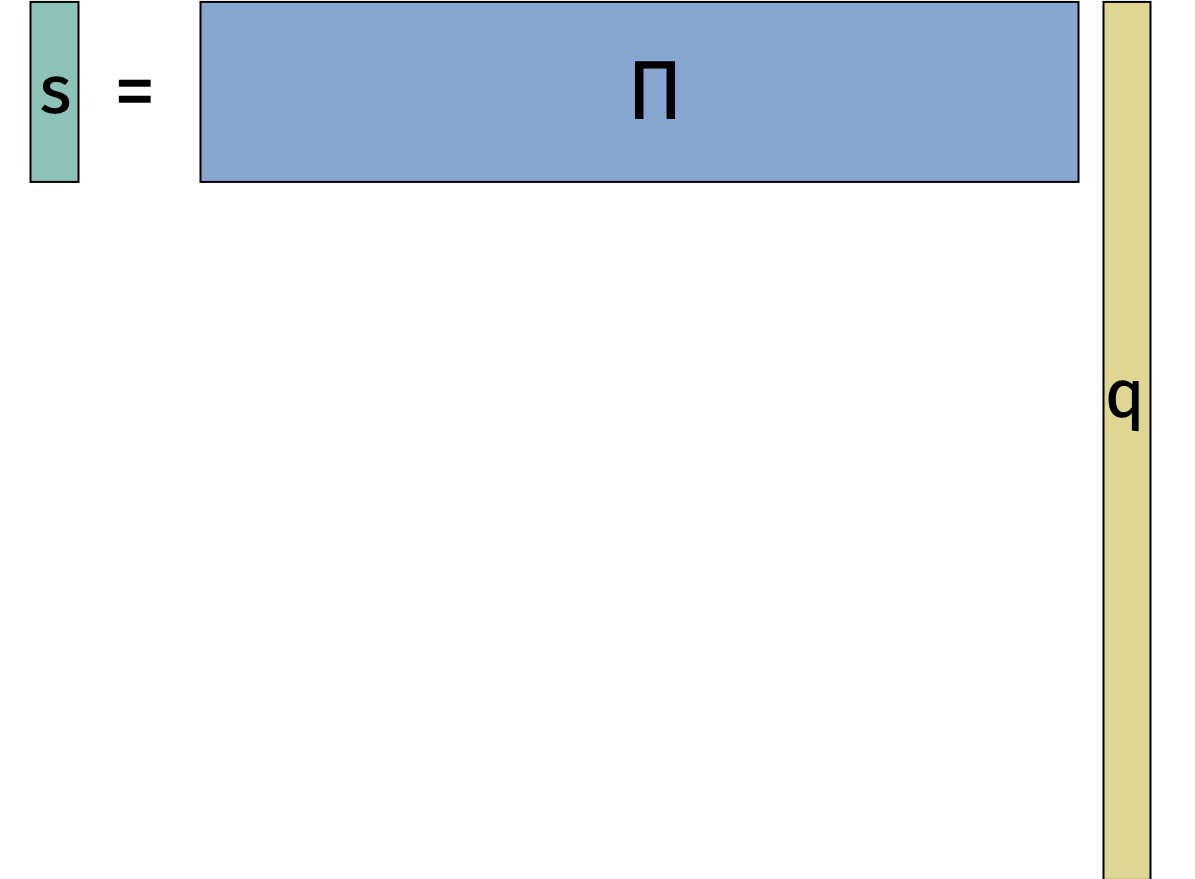
\includegraphics[height=.45\textheight]{jl_sketch.png}
	\end{center}
\end{frame}

\begin{frame}[t]
	\frametitle{sample application}
	\textbf{k-means clustering}: For data set $\bv{a}_1, \ldots, \bv{a}_n$,  find clusters $C_1, \ldots, C_k \subseteq \{1, \ldots, n\}$ to minimize:
	\vspace{-2em}
	
	\begin{align*}
		Cost(C_1,\ldots, C_k) = \sum_{j=1}^k \frac{1}{2|C_j|}\sum_{u,v\in C_j} \|\bv{a}_u - \bv{a}_v\|_2^2.
	\end{align*}
	
	\vspace{-2em}
	\begin{center}
		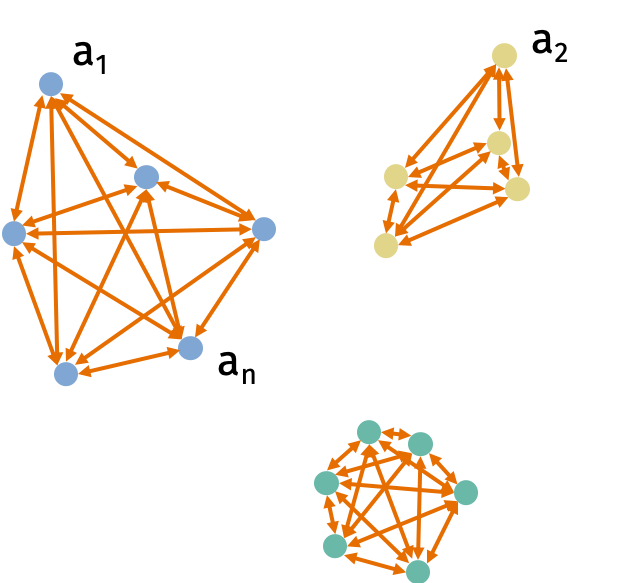
\includegraphics[width=.5\textwidth]{kmeans4.png}
	\end{center}
\end{frame}

\begin{frame}[t]
	\frametitle{sample application}
	\textbf{k-means clustering}: For data set $\bv{a}_1, \ldots, \bv{a}_n$,  find clusters $C_1, \ldots, C_k \subseteq \{1, \ldots, n\}$ to minimize:
	\vspace{-2em}
	
	\begin{align*}
		Cost(C_1,\ldots, C_k) = \sum_{j=1}^k \frac{1}{2|C_j|}\sum_{u,v\in C_j} \|\bv{a}_u - \bv{a}_v\|_2^2.
	\end{align*}
	
	\vspace{-2em}
	\begin{center}
		\vspace{-.5em}
		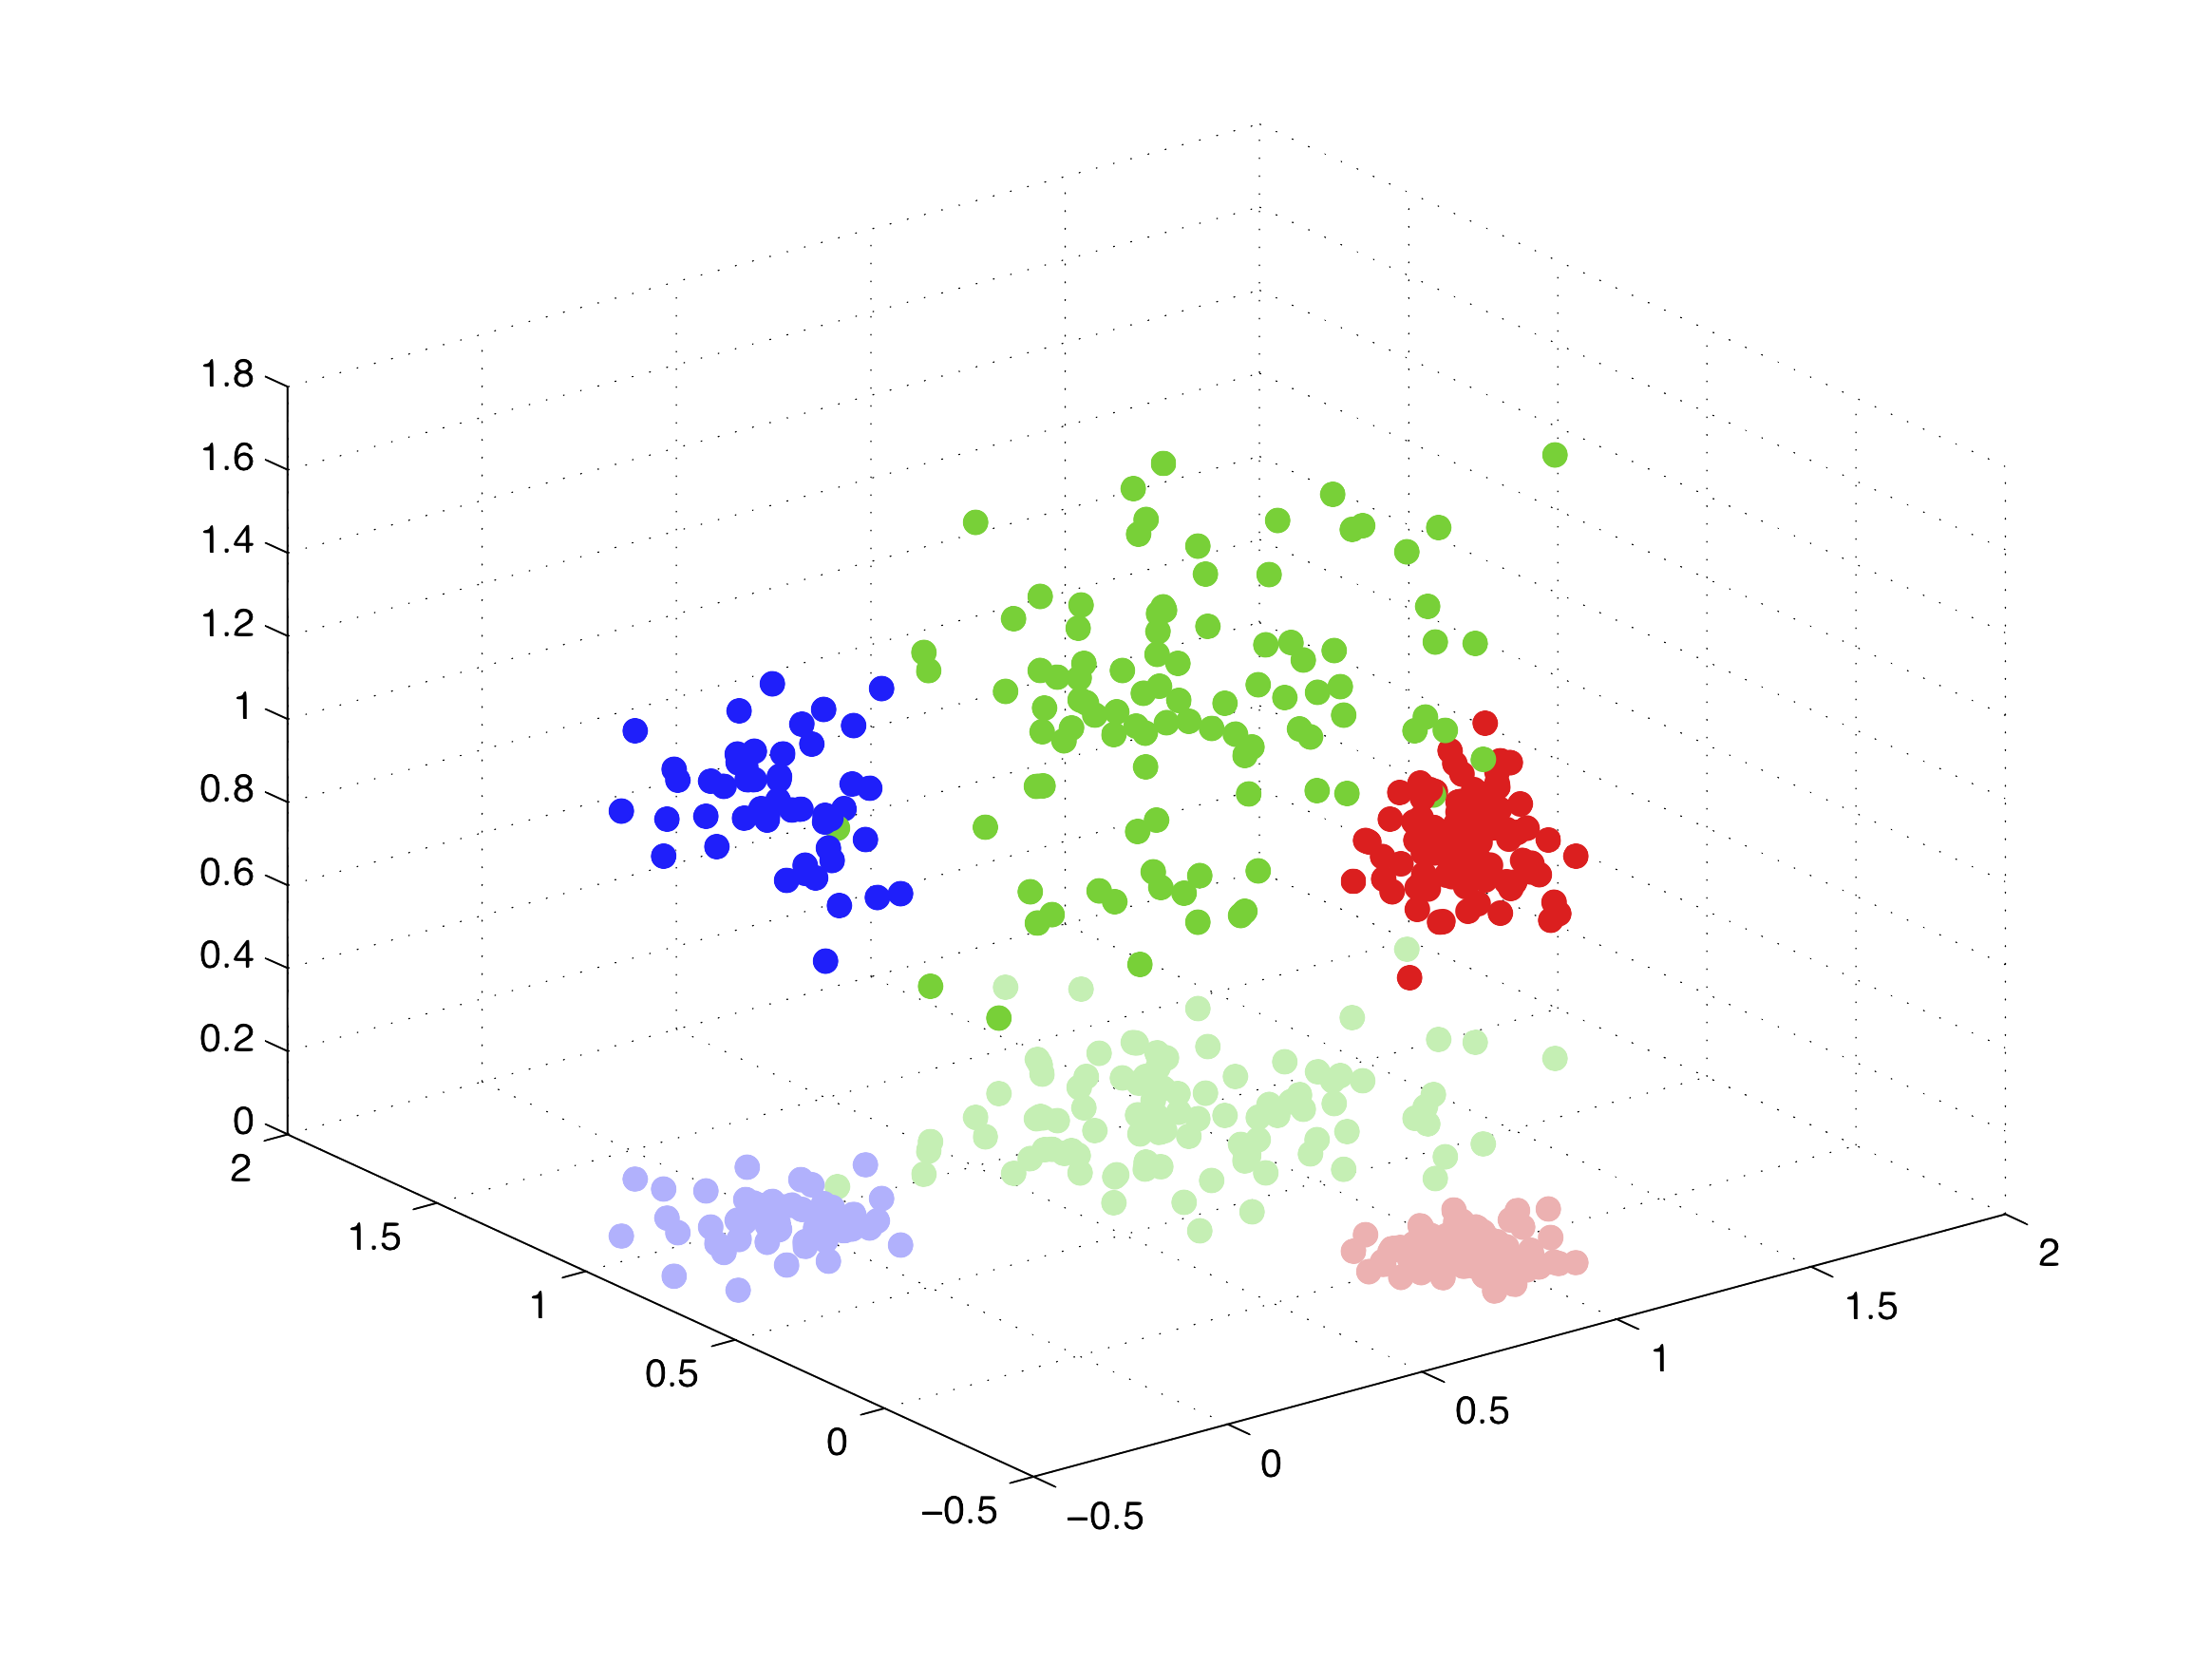
\includegraphics[width=.5\textwidth]{clustering_projected.png}
		\vspace{-.5em}
	\end{center}
	\textbf{Claim:} If I find the optimal clustering for $\bs{\Pi}\bv{a}_1, \ldots, \bs{\Pi}\bv{a}_n$ then its cost is less than $(1+\epsilon)$ times the cost of the best clustering obtained with the original data. 
\end{frame}

\begin{frame}[t]
	\frametitle{sample application}
	\textbf{k-means clustering}: Give data points $\bv{a}_1,\ldots, \bv{a}_n \in \R^d$, find centers $\bs{\mu}_1, \ldots, \bs{\mu}_k\in \R^d$ to minimize:
	\begin{align*}
		Cost(\bs{\mu}_1,\ldots, \bs{\mu}_k) = \sum_{i=1}^n \min_{j = 1,\ldots,k} \|\bs{\mu}_j - \bv{a}_i\|_2^2
	\end{align*}
	\begin{center}
		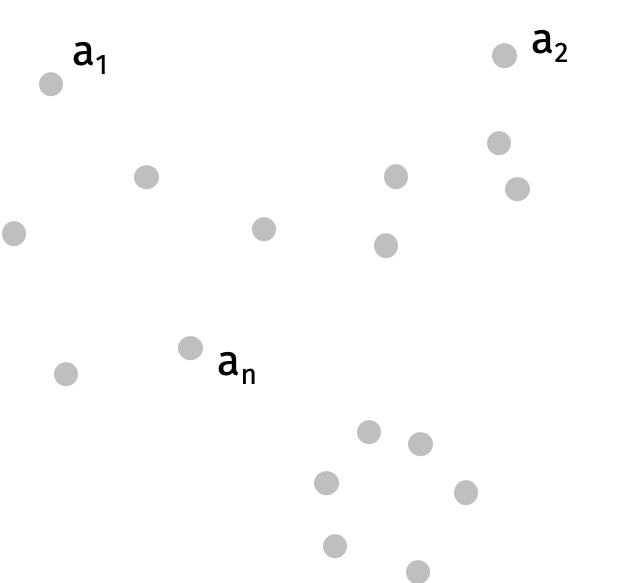
\includegraphics[width=.5\textwidth]{kmeans1.png}
	\end{center}
\end{frame}
\begin{frame}[t]
	\frametitle{sample application}
	\textbf{k-means clustering}: Give data points $\bv{a}_1,\ldots, \bv{a}_n \in \R^d$, find centers $\bs{\mu}_1, \ldots, \bs{\mu}_k\in \R^d$ to minimize:
	\begin{align*}
		Cost(\bs{\mu}_1,\ldots, \bs{\mu}_k) = \sum_{i=1}^n \min_{j = 1,\ldots,k} \|\bs{\mu}_j - \bv{a}_i\|_2^2
	\end{align*}
	\begin{center}
		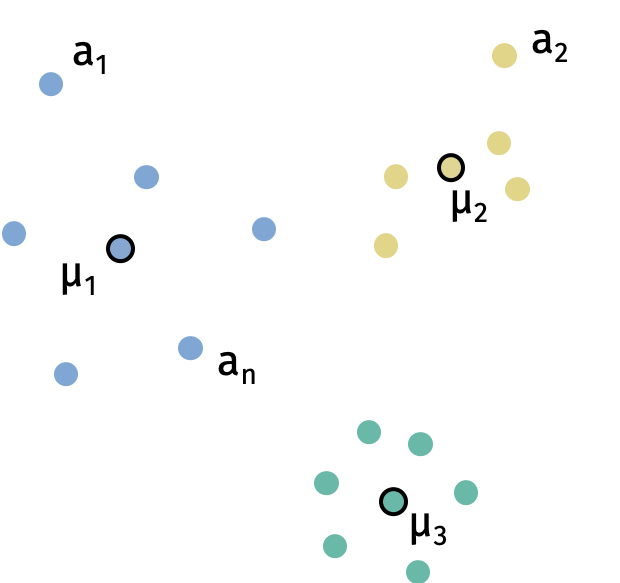
\includegraphics[width=.5\textwidth]{kmeans2.png}
	\end{center}
\end{frame}
\begin{frame}[t]
	\frametitle{sample application}
	\textbf{k-means clustering}: Give data points $\bv{a}_1,\ldots, \bv{a}_n \in \R^d$, find centers $\bs{\mu}_1, \ldots, \bs{\mu}_k\in \R^d$ to minimize:
	\begin{align*}
		Cost(\bs{\mu}_1,\ldots, \bs{\mu}_k) = \sum_{i=1}^n \min_{j = 1,\ldots,k} \|\bs{\mu}_j - \bv{a}_i\|_2^2
	\end{align*}
	\begin{center}
		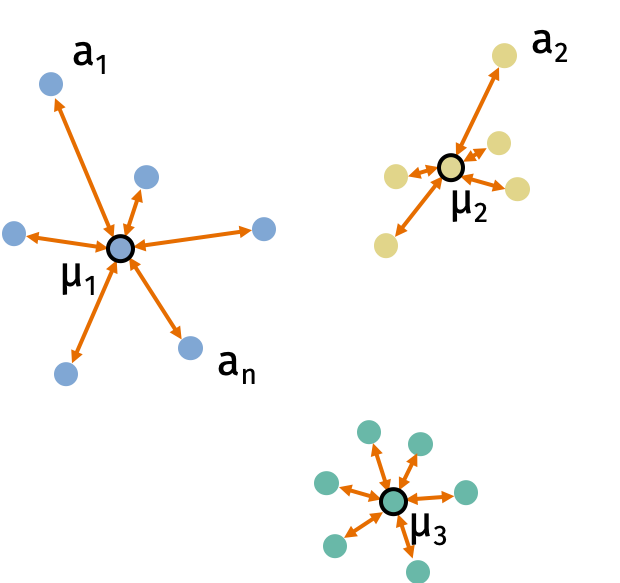
\includegraphics[width=.5\textwidth]{kmeans3.png}
	\end{center}
\end{frame}

\begin{frame}[t]
	\frametitle{k-means clustering}
	\textbf{Equivalent form}: Find clusters $C_1, \ldots, C_k \subseteq \{1, \ldots, n\}$ to minimize:
	\vspace{-3em}
	
	\begin{align*}
		Cost(C_1,\ldots, C_k) = \sum_{j=1}^k \frac{1}{2|C_j|}\sum_{u,v\in C_j} \|\bv{a}_u - \bv{a}_v\|_2^2.
	\end{align*}
	\vspace{-2em}
	\begin{center}
		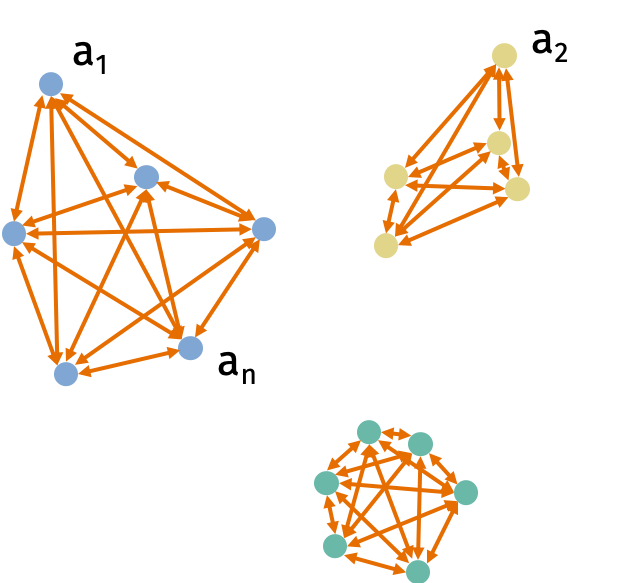
\includegraphics[width=.5\textwidth]{kmeans4.png}
	\end{center}
	\textbf{Exercise:} Prove this to your self.
\end{frame}

\begin{frame}[t]
	\frametitle{k-means clustering}
	NP hard to solve exactly, but there are many good approximation algorithms. All depend at least linearly on the dimension $d$. 
	
	\textbf{Approximation scheme}: Find clusters $\tilde{C}_1, \ldots, \tilde{C}_k$ for the $k = O\left(\frac{\log n}{\epsilon^2}\right)$ dimension data set $\bs{\Pi}\bv{a}_1, \ldots, \bs{\Pi}\bv{a}_n.$
	
	\vspace{-3em}
	\begin{center}
		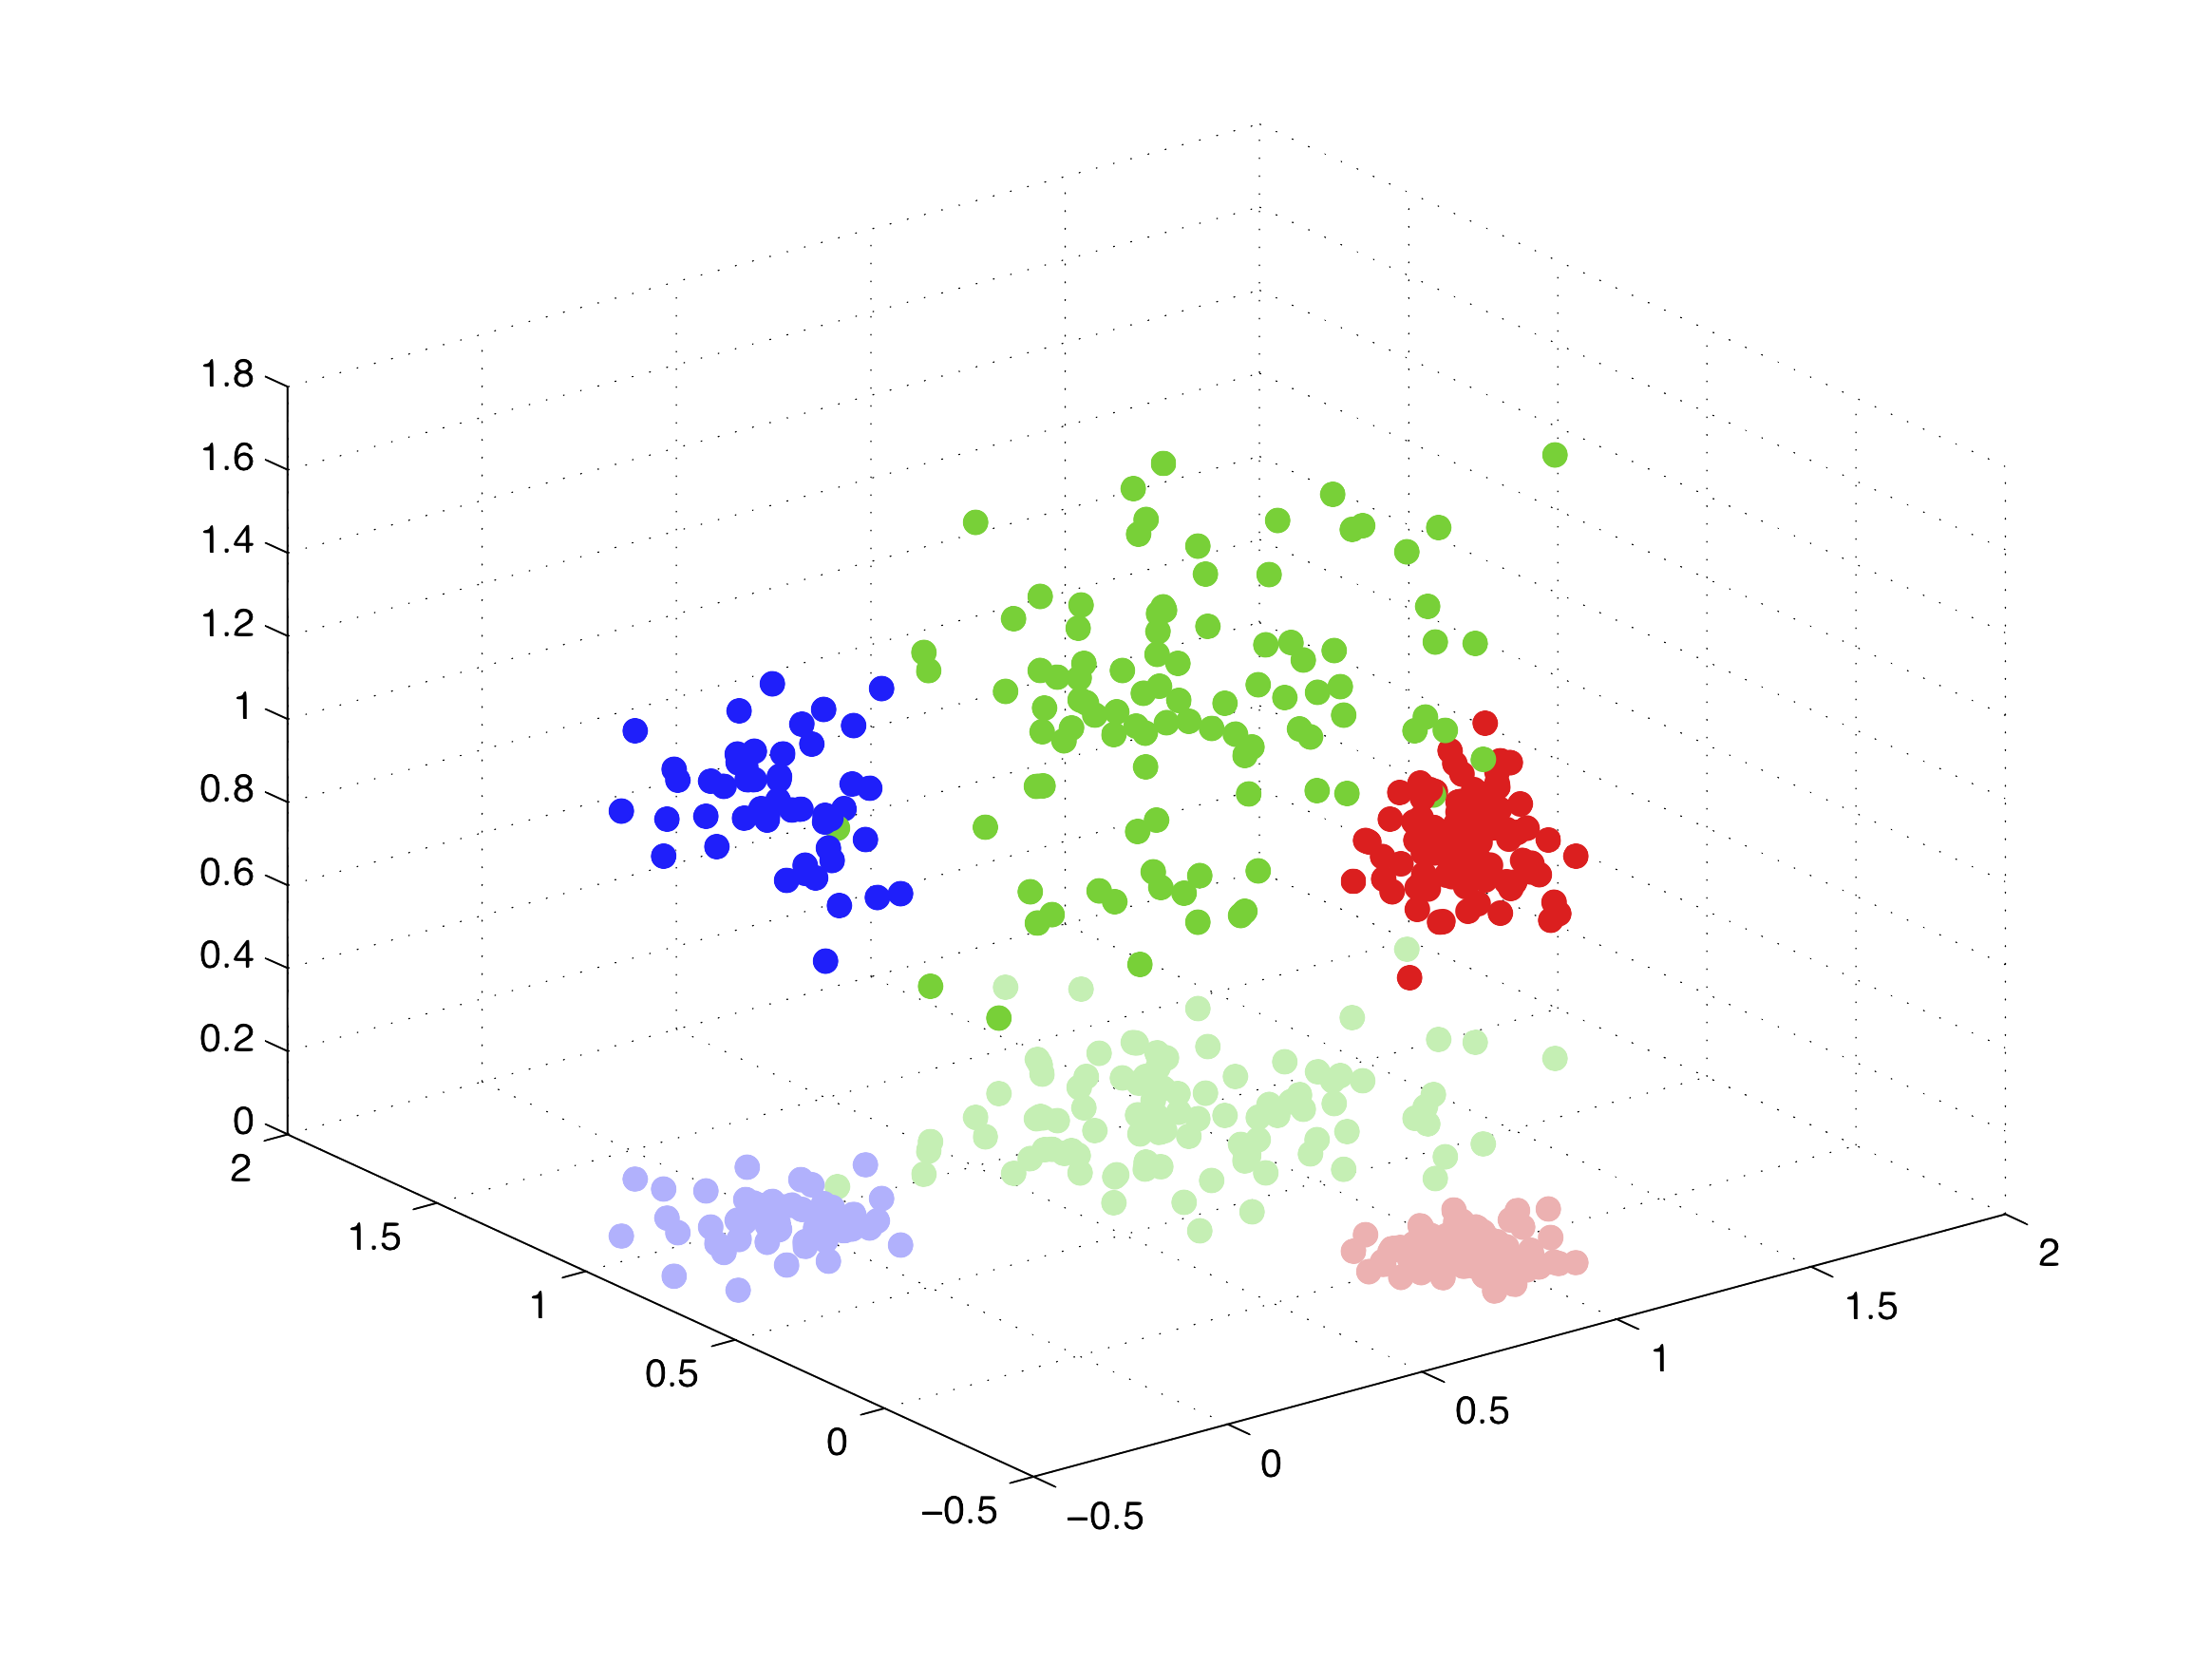
\includegraphics[width=.6\textwidth]{clustering_projected.png}
	\end{center}
	\vspace{-2em}
	Argue these clusters are near optimal for $\bv{a}_1, \ldots, \bv{a}_n$.
\end{frame}




\begin{frame}[t]
	\frametitle{k-means clustering}
	\begin{align*}
		Cost(C_1,\ldots, C_k) &= \sum_{j=1}^k \frac{1}{2|C_j|}\sum_{u,v\in C_j} \|\bv{a}_u - \bv{a}_v\|_2^2 \\
		\widetilde{Cost}(C_1,\ldots, C_k) &= \sum_{j=1}^k \frac{1}{2|C_j|}\sum_{u,v\in C_j} \|\Pi\bv{a}_u - \Pi\bv{a}_v\|_2^2
	\end{align*}
		
		
		\textbf{Claim:} For any clusters $C_1, \ldots, C_k$:
		\begin{align*}
	(1-\epsilon) Cost(C_1, \ldots, C_k) \leq \widetilde{Cost}(C_1, \ldots, C_k)   \leq  (1+\epsilon) Cost(C_1, \ldots, C_k) 
		\end{align*}
	
\end{frame}

\begin{frame}[t]
	\frametitle{k-means clustering}
	Suppose we use an approximation algorithm to find clusters $B_1, \ldots, B_k$ such that:
	\begin{align*}
		\widetilde{Cost}(B_1,\ldots, B_k) \leq (1+\alpha)\widetilde{Cost}^*
	\end{align*}
	
	Then: 
	\begin{align*}
		{Cost}(B_1,\ldots, B_k) &\leq \frac{1}{1-\epsilon}\widetilde{Cost}(B_1,\ldots, B_k) \\
		&\leq(1+O(\epsilon)) (1+\alpha)\widetilde{Cost}^*\\
		&\leq (1+O(\epsilon))(1+\alpha)(1+\epsilon){Cost}^*\\
		&= \alert{\left(1 + O(\alpha + \epsilon)\right){Cost}^*}
	\end{align*}

	\vspace{1em}
\begin{block}{\vspace*{-3ex}}
	\small ${Cost}^* = \min_{C_1, \ldots, C_k} Cost(C_1, \ldots, C_k)$ and $\widetilde{Cost}^* = \min_{C_1, \ldots, C_k} \widetilde{Cost}(C_1, \ldots, C_k) $
\end{block}
\end{frame}

\begin{frame}
	\frametitle{randomized jl constructions}
	\begin{center}
	 $\bs{\Pi} \in \R^{k\times d}$ can chosen so that each entry equals $\frac{1}{\sqrt{k}}  \mathcal{N}(0,1)$, or each entry equals $\frac{1}{\sqrt{k}}  \pm 1$ with equal probability. 
	\end{center}
	\vspace{1em}
	
	\begin{columns}
		\begin{column}{0.5\textwidth}
			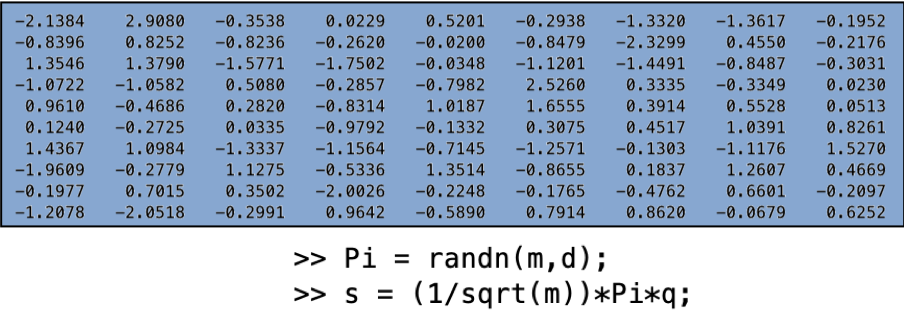
\includegraphics[width=\textwidth]{rand_gauss.png}
		\end{column}
		\begin{column}{0.5\textwidth}
			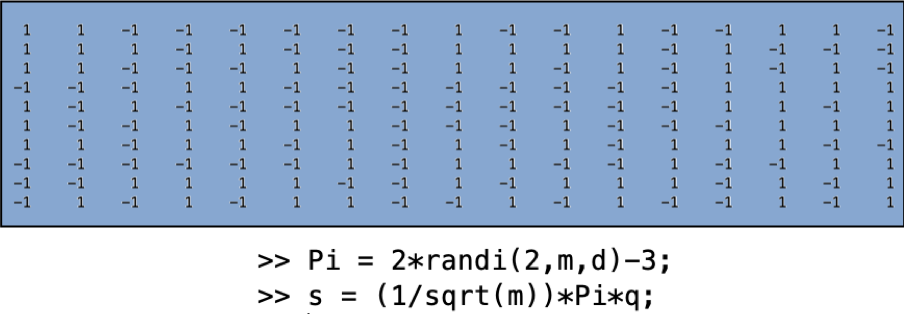
\includegraphics[width=\textwidth]{rand_sign.png}
		\end{column}
	\end{columns}
	
	\begin{center}
		Lots of other constructions work.
	\end{center}
\end{frame}

\begin{frame}
	\frametitle{random projection}
	\begin{center}
		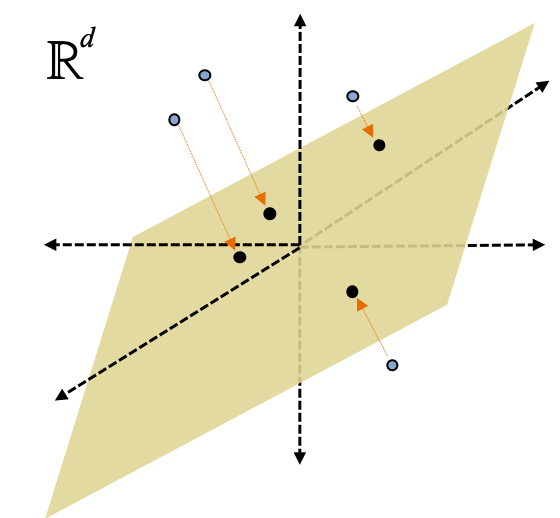
\includegraphics[width=.6\textwidth]{random_projection.png}
	\end{center}
	\textbf{Intuition:} Multiplying by a random matrix mimics the process of projecting onto a random $k$ dimensional subspace in $d$ dimensions.
\end{frame}

\begin{frame}
	\frametitle{euclidean dimensionality reduction}
	\textbf{Intermediate result:}
	\begin{lemma}[Distributional JL Lemma]
		Let $\bs{\Pi} \in \R^{k\times d}$ be chosen so that each entry equals $\frac{1}{\sqrt{k}}  \mathcal{N}(0,1)$, where $\mathcal{N}(0,1)$ denotes a standard Gaussian random variable. 
		
		If we choose $k = O\left(\frac{\log(1/\delta)}{\epsilon^2}\right)$, then for \emph{any vector $\bv{x}$}, with probability $(1-\delta)$:
		\begin{align*}
			(1-\epsilon)\|\bv{x}\|_2^2 \leq \|\bs{\Pi}\bv{x}\|_2^2 \leq (1+\epsilon) \|\bv{x}\|_2^2
		\end{align*}
	\end{lemma}
	
	\begin{center}\alert{
			\textbf{Given this lemma, how do we prove the traditional Johnson-Lindenstrauss lemma?}}
	\end{center}
\end{frame}

\begin{frame}
	\frametitle{jl from distributional jl}
	We have a set of vectors $\bv{q}_1, \ldots, \bv{q}_n$. Fix $i,j \in 1,\ldots, n$. 
	
	Let $\bv{x} = \bv{q}_i - \bv{q}_j$. By linearity, $\bs{\Pi}\bv{x} = \bs{\Pi}(\bv{q}_i - \bv{q}_j) = \bs{\Pi}\bv{q}_i - \bs{\Pi}\bv{q}_j$.
	
	By the Distributional JL Lemma, with probability $1-\delta$,
	\begin{align*}
		(1-\epsilon)\|\bv{q}_i - \bv{q}_j\|_2 \leq \|\bs{\Pi}\bv{q}_i - \bs{\Pi}\bv{q}_j\|_2 \leq (1+\epsilon) \|\bv{q}_i - \bv{q}_j\|_2.
	\end{align*}
	Finally, set $\delta = \frac{1}{n^2}$. Since there are $< n^2$ total $i,j$ pairs, by a union bound we have that with probability $9/10$, the above will hold \emph{for all} $i,j$, as long as we compress to:
	
	\begin{align*}
		k = O\left(\frac{\log(1/(1/n^2))}{\epsilon^2}\right) = O\left(\frac{\log n}{\epsilon^2}\right) \text{ dimensions.}\qed
	\end{align*}
	
\end{frame}

\begin{frame}
	\frametitle{proof of distributional jl}
	Want to argue that, with probability $(1-\delta)$,
	\begin{align*}
		(1-\epsilon)\|\bv{x}\|_2^2 \leq |\bs{\Pi}\bv{x}\|_2^2 \leq (1+\epsilon)\|\bv{x}\|_2^2 
	\end{align*}
	
	\begin{center}
		\alert{\textbf{Claim}: $\E \|\bs{\Pi} \bv{x} \|_2^2 = \|\bv{x}\|_2^2.$}
	\end{center}
	
	\vspace{-1em}
	Some notation:
	\begin{center}
		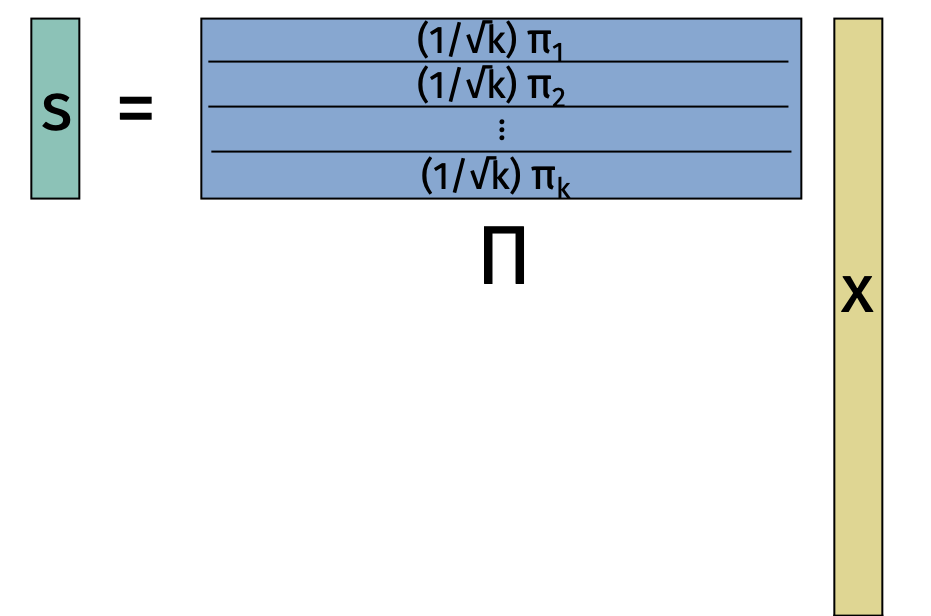
\includegraphics[width=.6\textwidth]{jl_notation.png}
		
		So each $\bs{\pi}_i$ contains $\mathcal{N}(0,1)$ entries. 
	\end{center}
\end{frame}

\begin{frame}
	\frametitle{proof of distributional jl}
	\textbf{Intermediate Claim:} Let $\bs{\pi}$ be a length $d$ vector with $\mathcal{N}(0,1)$ entries. 
	\begin{align*}
		\E\left[\|\bs{\Pi} \bv{x} \|_2^2 \right]  = \E\left[\left(\langle\bs{\pi},\bv{x}\rangle\right)^2 \right] .
	\end{align*}
	%	\begin{align*}
		%		\|\bs{\Pi} \bv{x} \|_2^2 = \sum_i^k \bv{s}[i]^2 = \sum_i^k \left(\frac{1}{\sqrt{k}}\langle\bs{\pi}_i,\bv{x}\rangle\right)^2 = \frac{1}{k}\sum_i^k \left(\langle\bs{\pi}_i,\bv{x}\rangle\right)^2 
		%	\end{align*}
	%	\begin{align*}
		%		\E\left[\|\bs{\Pi} \bv{x} \|_2^2 \right] &= \frac{1}{k}\sum_i^k \E\left[\left(\langle\bs{\pi}_i,\bv{x}\rangle\right)^2 \right] \\
		%		& =\E\left[\left(\langle\bs{\pi}_i,\bv{x}\rangle\right)^2 \right] 
		%	\end{align*}
	\vspace{9em}
	\begin{block}{\vspace*{-3ex}}
		\small \textbf{Goal}: Prove $\E \|\bs{\Pi} \bv{x} \|_2^2 = \|\bv{x}\|_2^2$.
	\end{block}
\end{frame}

\begin{frame}
	\frametitle{proof of distributional jl}	
	\begin{align*}
		\langle\bs{\pi},\bv{x}\rangle = Z_1\cdot\bv{x}[1] + Z_2\cdot\bv{x}[2]  +  \ldots + Z_d\cdot\bv{x}[d]
	\end{align*}
	where each $Z_1, \ldots, Z_d$ is a standard normal $\mathcal{N}(0,1)$. 
	
	We have that $Z_i \cdot\bv{x}[i]$ is a normal $\mathcal{N}(0,\bv{x}[i]^2)$ random variable.
	
	\vspace{5em}
	\begin{block}{\vspace*{-3ex}}
		\small \textbf{Goal}: Prove $\E \|\bs{\Pi} \bv{x} \|_2^2 = \|\bv{x}\|_2^2$. Established: $\E \|\bs{\Pi} \bv{x} \|_2^2 = \E\left[\left(\langle\bs{\pi},\bv{x}\rangle\right)^2 \right]$
	\end{block}
\end{frame}

\begin{frame}[t]
	\frametitle{stable random variables}
	\textbf{What type of random variable is $\langle\bs{\pi},\bv{x}\rangle$?}
	\begin{fact}[Stability of Gaussian random variables]
		\begin{align*}
			\mathcal{N}(\mu_1, \sigma_1^2) + \mathcal{N}(\mu_2, \sigma_2^2) =  \mathcal{N}(\mu_1 + \mu_2, \sigma_1^2 + \sigma_2^2)
		\end{align*}
	\end{fact}
	\begin{align*}
		\langle\bs{\pi},\bv{x}\rangle &= \mathcal{N}(0,\bv{x}[1]^2) + \mathcal{N}(0,\bv{x}[2]^2) + \ldots + \mathcal{N}(0,\bv{x}[d]^2) \\ &= \mathcal{N}(0,\|\bv{x}\|_2^2). 
	\end{align*}
	
	So $\E \|\bs{\Pi} \bv{x} \|_2^2 = \E\left[\left(\langle\bs{\pi},\bv{x}\rangle\right)^2 \right] = \E\left[\mathcal{N}(0,\|\bv{x}\|_2^2)\right]  = \|\bv{x}\|_2^2$, as desired.
\end{frame}

\begin{frame}
	\frametitle{proof of distributional jl}
	Want to argue that, with probability $(1-\delta)$,
	\begin{align*}
		(1-\epsilon)\|\bv{x}\|_2^2 \leq \|\bs{\Pi}\bv{x}\|_2^2 \leq (1+\epsilon)\|\bv{x}\|_2^2 
	\end{align*}
	
	\begin{enumerate}
		\item $\E \|\bs{\Pi} \bv{x} \|_2^2 = \|\bv{x}\|_2^2$.
		\item Need to use a concentration bound.
	\end{enumerate}
	\begin{align*}
		\|\bs{\Pi} \bv{x} \|_2^2 = \frac{1}{k}\sum_{i=1}^k \left(\langle\bs{\pi}_i,\bv{x}\rangle\right)^2 = \frac{1}{k}\sum_{i=1}^k \mathcal{N}(0,\|\bv{x}\|_2^2)
	\end{align*}
	\alert{``Chi-squared random variable with $k$ degrees of freedom.''}
\end{frame}

\begin{frame}[t]
	\frametitle{concentration of chi-squared random variables}
	\begin{lemma} Let $Z$ be a Chi-squared random variable with $k$ degrees of freedom. 
		\begin{align*}
			\Pr[|\E Z - Z| \geq \epsilon \E Z] \leq 2 e^{-k\epsilon^2/8}
		\end{align*}
	\end{lemma}
	
	\vspace{8em}
	\begin{block}{\vspace*{-3ex}}
		\small \textbf{Goal}: Prove $\|\bs{\Pi} \bv{x} \|_2^2$ concentrates within $1 \pm \epsilon$ of its expectation, which equals $\|\bv{x} \|_2^2$.
	\end{block}
\end{frame}

\begin{frame}
	\frametitle{connection last lecture}
	If high dimensional geometry is so different from low-dimensional geometry, why is \emph{dimensionality reduction possible?} Doesn't Johnson-Lindenstrauss tell us that high-dimensional geometry can be approximated in low dimensions?
\end{frame}

\begin{frame}[t]
	\frametitle{connection to dimensionality reduction}
	\textbf{Hard case:} $\bv{x}_1, \ldots, \bv{x}_n \in \R^d$ are all mutually orthogonal unit vectors: 
	\begin{align*}
		\|\bv{x}_i - \bv{x}_j\|_2^2 &= 2 & &\text{for all $i,j$.}  
	\end{align*}
	When we reduce to $k$ dimensions with JL, we still expect these vectors to be nearly orthogonal. Why?
	
\end{frame}

\begin{frame}[t]
	\frametitle{connection to dimensionality reduction}
	\textbf{Hard case:} $\bv{x}_1, \ldots, \bv{x}_n \in \R^d$ are all mutually orthogonal unit vectors: 
	\begin{align*}
		\|\bv{x}_i - \bv{x}_j\|_2^2 &= 2 & &\text{for all $i,j$.}  
	\end{align*}
	
	From our result earlier, in $O(\log n /\epsilon^2)$ dimensions, there exists $2^{O(\epsilon^2\cdot \log n /\epsilon^2)} \geq n $ unit vectors that are close to mutually orthogonal.
	\alert{$O(\log n /\epsilon^2)$ = \emph{just enough} dimensions.}
	\vspace{2em}
	
	\textbf{Alternative view:} Without additional structure, we expect that learning/inference in $d$ dimenions requires $2^{O(d)}$ data points. If we really had a data set that large, then the JL bound would be vacous, since $\log(n) = O(d)$.
\end{frame}


%\begin{frame}[standout]
%	\begin{center}
	%		break
	%	\end{center}
%\end{frame}
%
\begin{frame}
	\frametitle{dimensionality reduction}
	\begin{center}
		The Johnson-Lindenstrauss Lemma let us sketch vectors and preserve their $\ell_2$ Euclidean distance. 
		
		We also have dimensionality reduction techniques that preserve alternative measures of similarity.
	\end{center}
\end{frame}


\begin{frame}
	\frametitle{similarity estimation}
	\begin{center}
			How does \textbf{Shazam} match a song clip against a library of 8 million songs (32 TB of data) in a fraction of a second?
			
			\only<1>{
\includegraphics[width=.4\textwidth]{shazam.png}}
		\end{center}
	\vspace{-1em}
	\uncover<2->{
			\begin{figure}[h]
					\centering
					\begin{subfigure}[t]{0.35\textwidth}
							\centering
							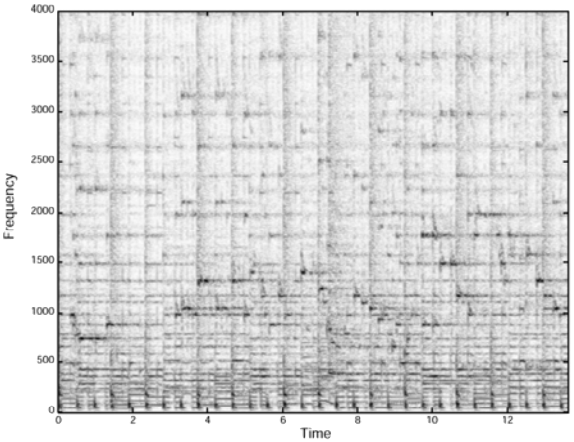
\includegraphics[width=\textwidth]{spectrogram.png}
							\caption{Spectrogram extracted from audio clip.}
						\end{subfigure}
					~
					\begin{subfigure}[t]{0.35\textwidth}
							\centering
							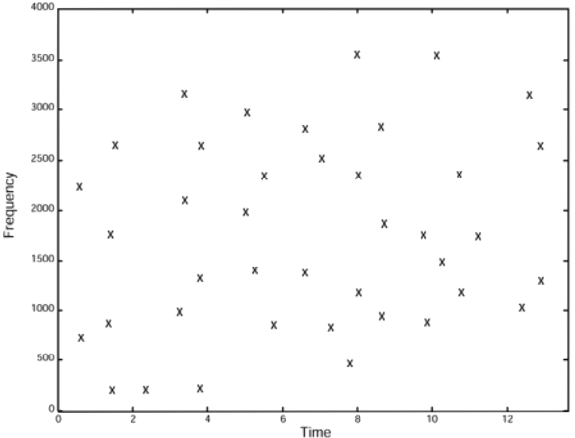
\includegraphics[width=\textwidth]{spectrogramThresh.png}
							\caption{Processed spectrogram: used to construct audio ``fingerprint'' $\textbf{q}\in \{0,1\}^d$.}
						\end{subfigure}
				\end{figure}
			
			\uncover<2->{\vspace{-.5em}
					Each clip is represented by a high dimensional binary vector $\bv{q}$.
					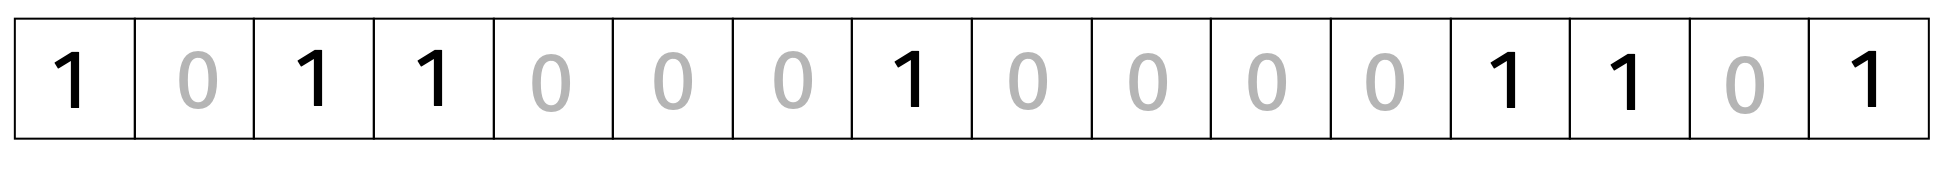
\includegraphics[width=\textwidth]{binaryVector.png}
				}
		}
\end{frame}


\begin{frame}
	\frametitle{dimensionality reduction}
	\begin{center}
		The Johnson-Lindenstrauss Lemma let us sketch vectors and preserve their $\ell_2$ Euclidean distance. 
		
		We also have dimensionality reduction techniques that preserve alternative measures of similarity.
	\end{center}
\end{frame}

\begin{frame}
	\frametitle{similarity estimation}
	\begin{center}
			Given $\textbf{q}$, find any nearby ``fingerprint'' $\bv{y}$  in a database -- i.e. any $\bv{y}$ with $\text{dist}(\bv{y}, \bv{q})$ small. 
		\end{center}
	
		\textbf{Challenges}:
		\begin{itemize}
				\item Database is possibly huge: $O(nd)$ bits.
				\item Expensive to compute $\text{dist}(\bv{y},\bv{q})$: $O(d)$ time.
			\end{itemize}
\end{frame}

\begin{frame}
	\frametitle{similarity estimation}
	\textbf{Goal:} Design a more compact sketch for comparing $\bv{q}, \bv{y}\in \{0,1\}^d$. Ideally $\ll d$ space/time complexity.
		\begin{align*}
				C(\textbf{q}) \in \R^k \\	
				C(\textbf{y}) \in \R^k 
			\end{align*}
		\begin{center}
				\vspace{-.5em}
				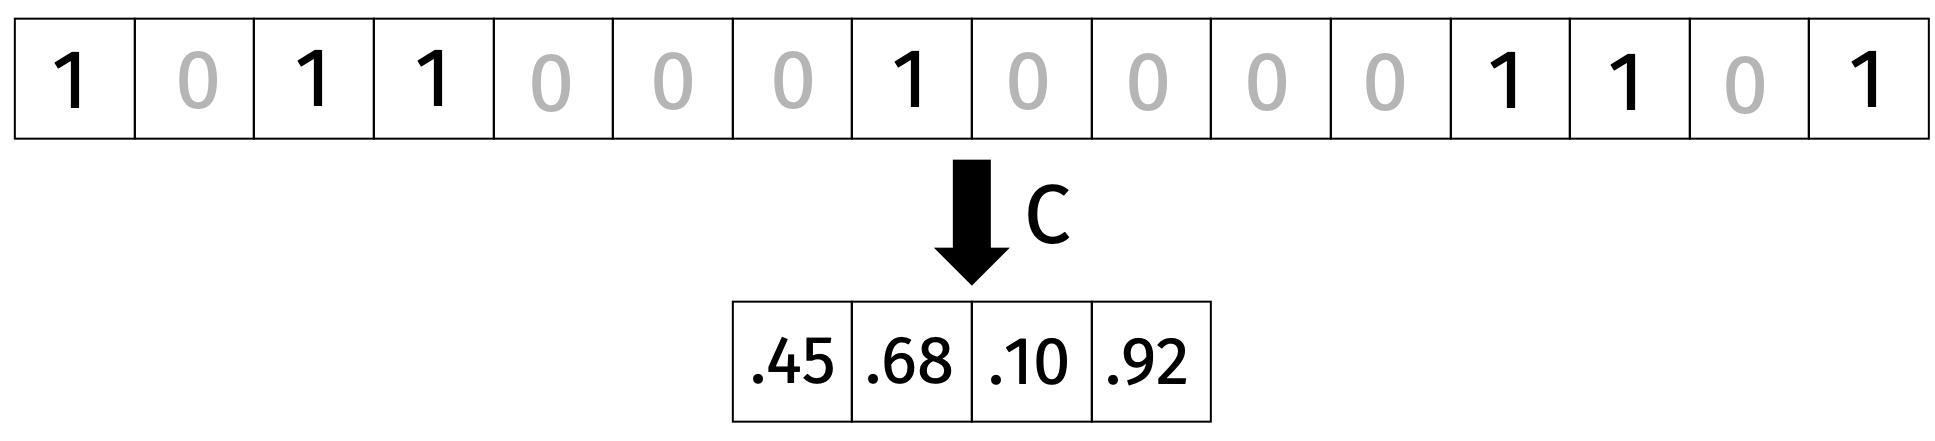
\includegraphics[width=.8\textwidth]{compression.png}
				\vspace{-.5em}
			\end{center}
			As in Johnson-Lindenstrauss compressions, we want that	$C(\bv{q})$ is similar to $C(\bv{y})$ if $\bv{q}$ is similar to $\bv{y}$.
\end{frame}

\begin{frame}
	\frametitle{jaccard similarity}
	\begin{definition}[Jaccard Similarity]
			\begin{align*}
					J(\bv{q},\bv{y}) = \frac{|\bv{q} \cap \bv{y}|}{|\bv{q} \cup \bv{y}|} = \frac{\text{\# of non-zero entries in common}}{\text{total \# of non-zero entries}}
				\end{align*}
			Natural similarity measure for binary vectors. $0\leq J(\bv{q},\bv{y})\leq 1$.
		\end{definition}
	
	Can be applied to any data which has a natural binary representation (more than you might think). 
\end{frame}

\begin{frame}
	\frametitle{jaccard similarity for document comparison}
	\textbf{``Bag-of-words'' model:}
	\begin{center}
			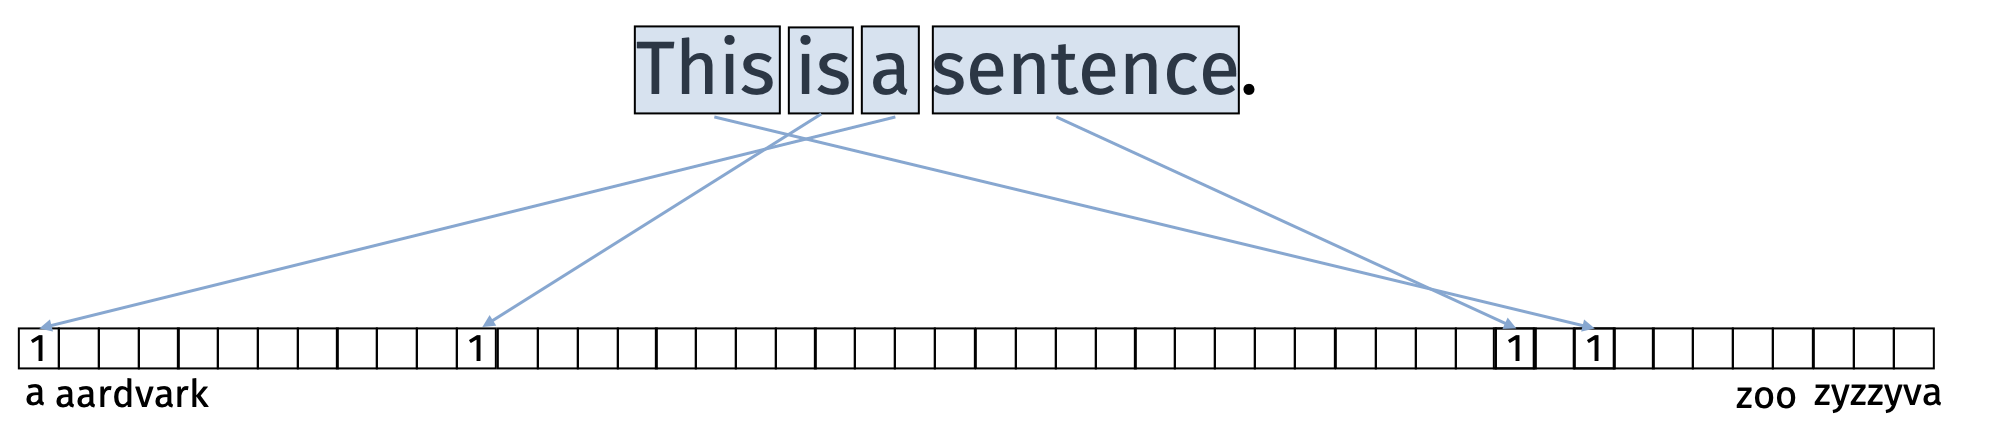
\includegraphics[width=.95\textwidth]{bagofwords.png}
		\end{center}
	
	How many words do a pair of documents have in common?
\end{frame}

\begin{frame}
	\frametitle{jaccard similarity for document comparison}
	\textbf{``Bag-of-words'' model:}
	\begin{center}
			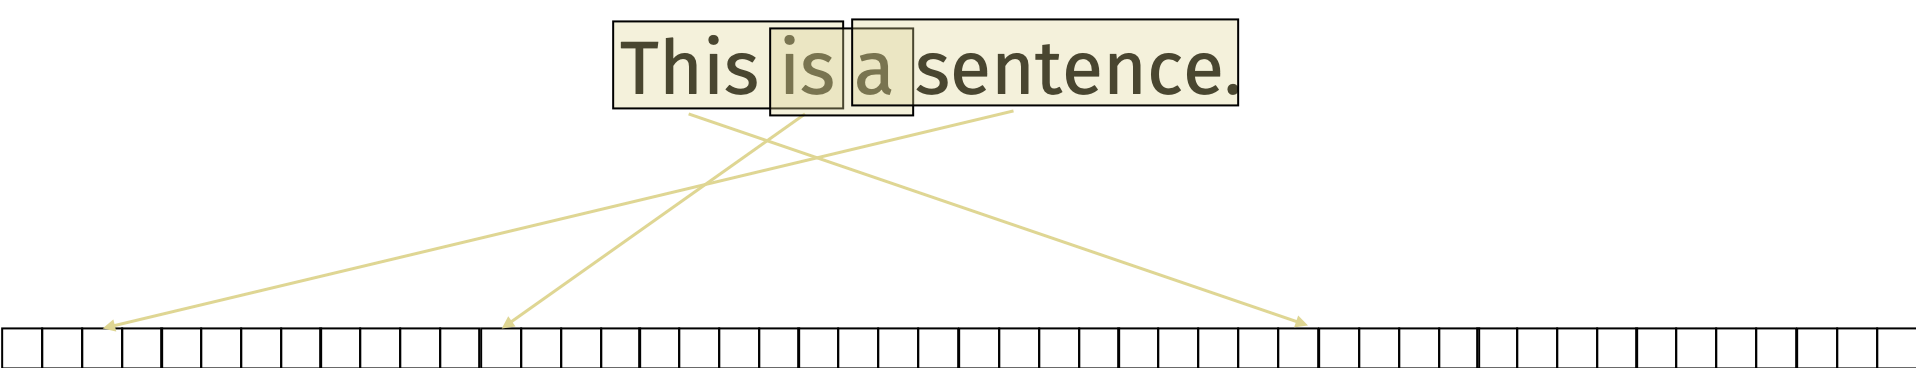
\includegraphics[width=.95\textwidth]{bigrams.png}
		\end{center}
	
	How many bigrams do a pair of documents have in common?
\end{frame}

\begin{frame}
	\frametitle{jaccard similarity for seismic data}
	\begin{center}
			\vspace{-.5em}
			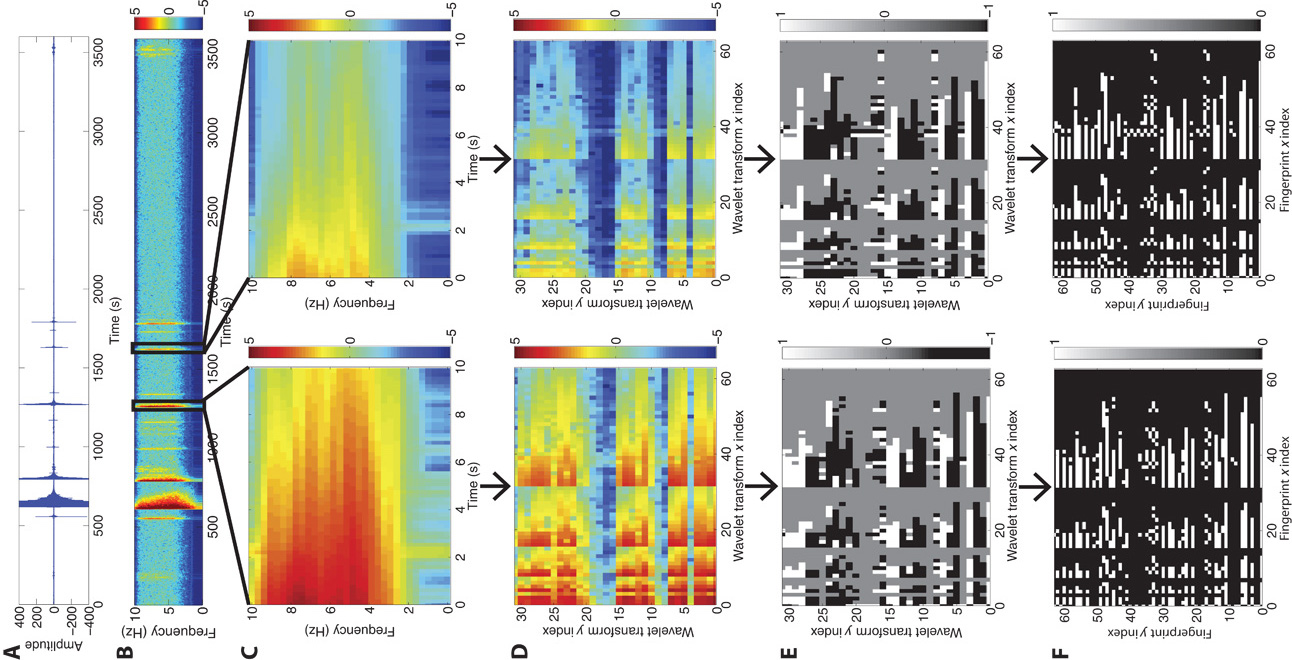
\includegraphics[width=.6\textwidth]{earthquakeFeatures.jpg}
			
			\vspace{-.5em}
			Feature extract pipeline for earthquake data.
			
			(see paper by Rong et al. posted on course website)
		\end{center}
\end{frame}

\begin{frame}
	\frametitle{applications: document similarity}
	\begin{itemize}
			\item Finding duplicate or new duplicate documents or webpages.
			\item Change detection for high-speed web caches.
			\item Finding near-duplicate emails or customer reviews which could indicate spam.
		\end{itemize}
	
\end{frame}


\begin{frame}
	\frametitle{similarity estimation}
	\textbf{Goal:} Design a compact sketch $C: \{0,1\}\rightarrow \R^k$:
	\begin{center}
			\vspace{-.5em}
			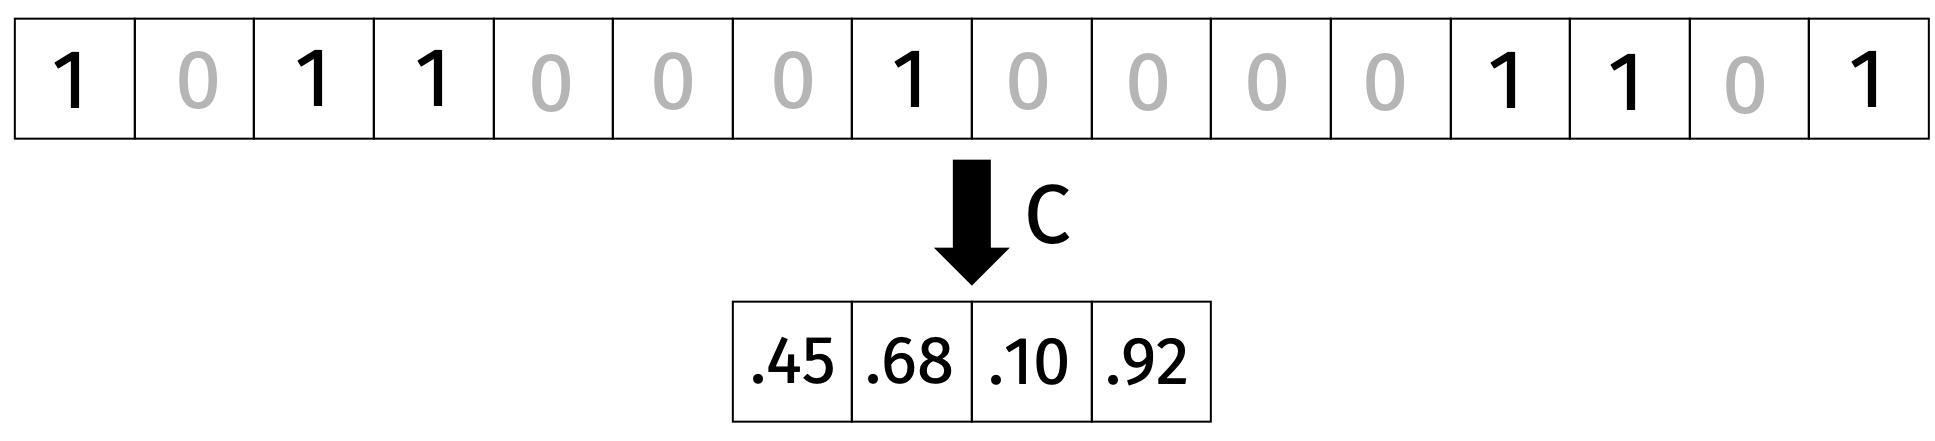
\includegraphics[width=.8\textwidth]{compression.png}
			\vspace{-.5em}
		\end{center}
	Want to use $C(\bv{q}), C(\bv{y})$ to approximately compute the Jaccard similarity $J(\bv{q},\bv{y}) = \frac{|\bv{q} \cap \bv{y}|}{|\bv{q} \cup \bv{y}|}$.
\end{frame}

\begin{frame}
	\frametitle{minhash}
	\textbf{MinHash (Broder, '97)}:
	\begin{itemize}
		\item Choose $k$ random hash functions $h_1, \ldots, h_k: \{1,\ldots, n\} \rightarrow [0,1]$. 
		\item For $i\in 1, \ldots,k$, 
		\begin{itemize}
			\item Let $c_i = \min_{j, \bv{q}_j = 1} h_i(j)$.
		\end{itemize}
		\item $C(\bv{q}) = [c_1, \ldots, c_k]$.
	\end{itemize}
	\begin{center}
		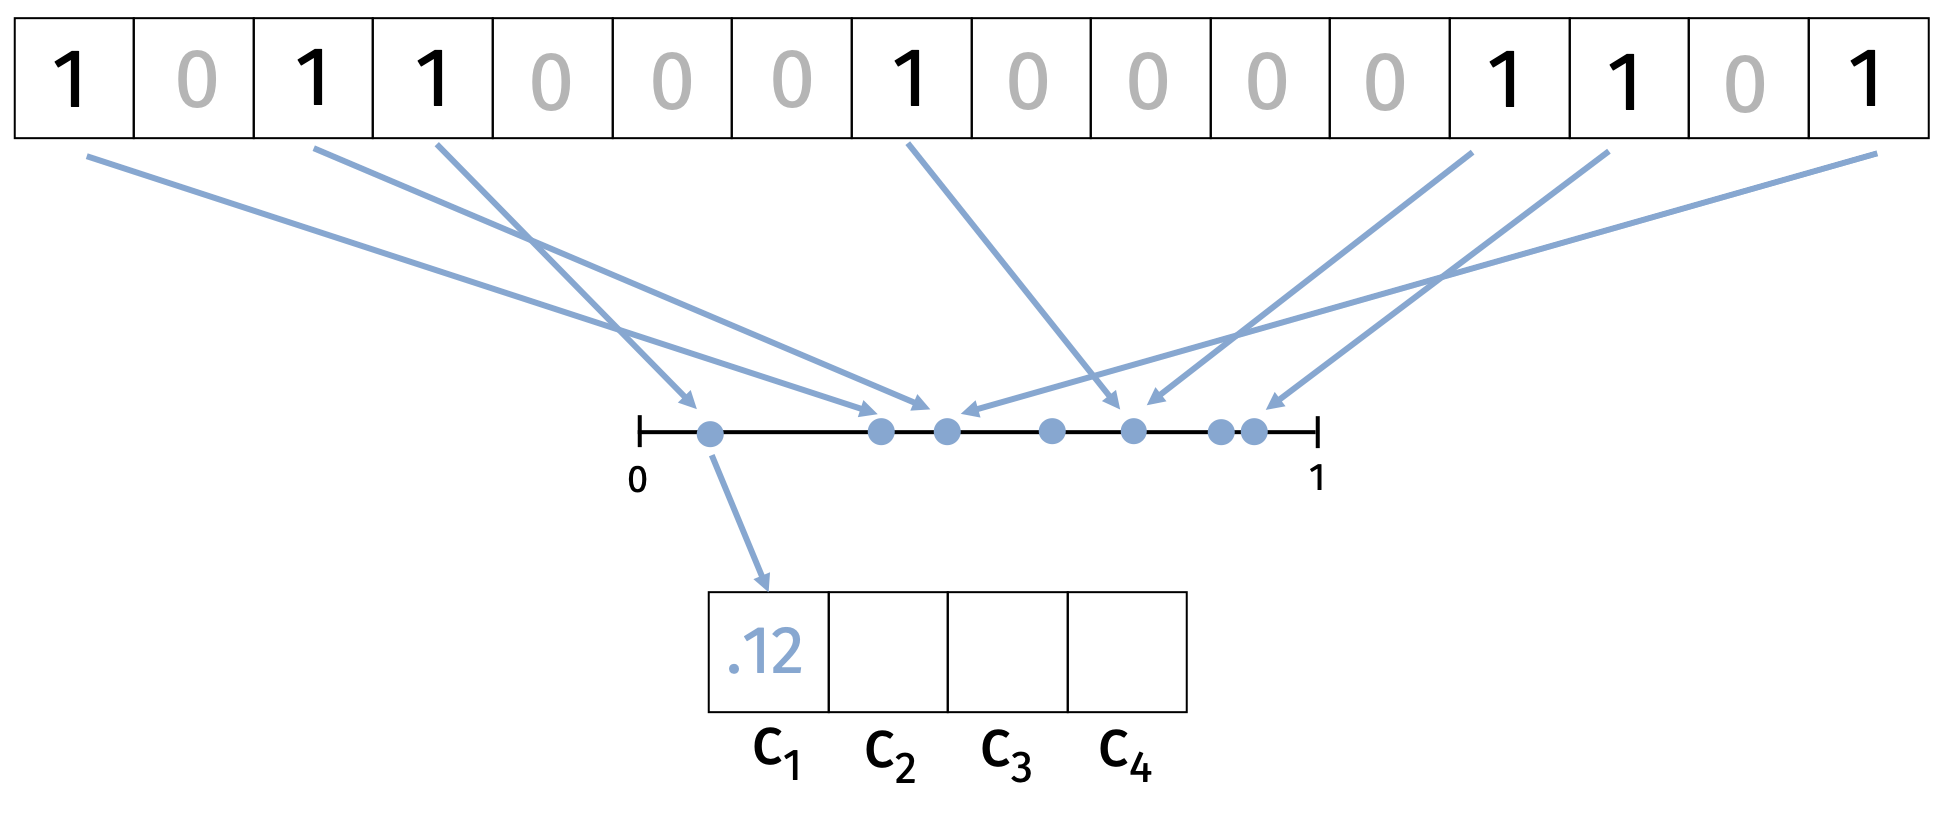
\includegraphics[width=\textwidth]{minHash1.png}	
	\end{center}
\end{frame}

\begin{frame}
	\frametitle{minhash}
	\begin{itemize}
		\item Choose $k$ random hash functions $h_1, \ldots, h_k: \{1,\ldots, n\} \rightarrow [0,1]$. 
		\item For $i\in 1, \ldots,k$, 
		\begin{itemize}
			\item Let $c_i = \min_{j, \bv{q}_j = 1} h_i(j)$.
		\end{itemize}
		\item $C(\bv{q}) = [c_1, \ldots, c_k]$.
	\end{itemize}
	\begin{center}
		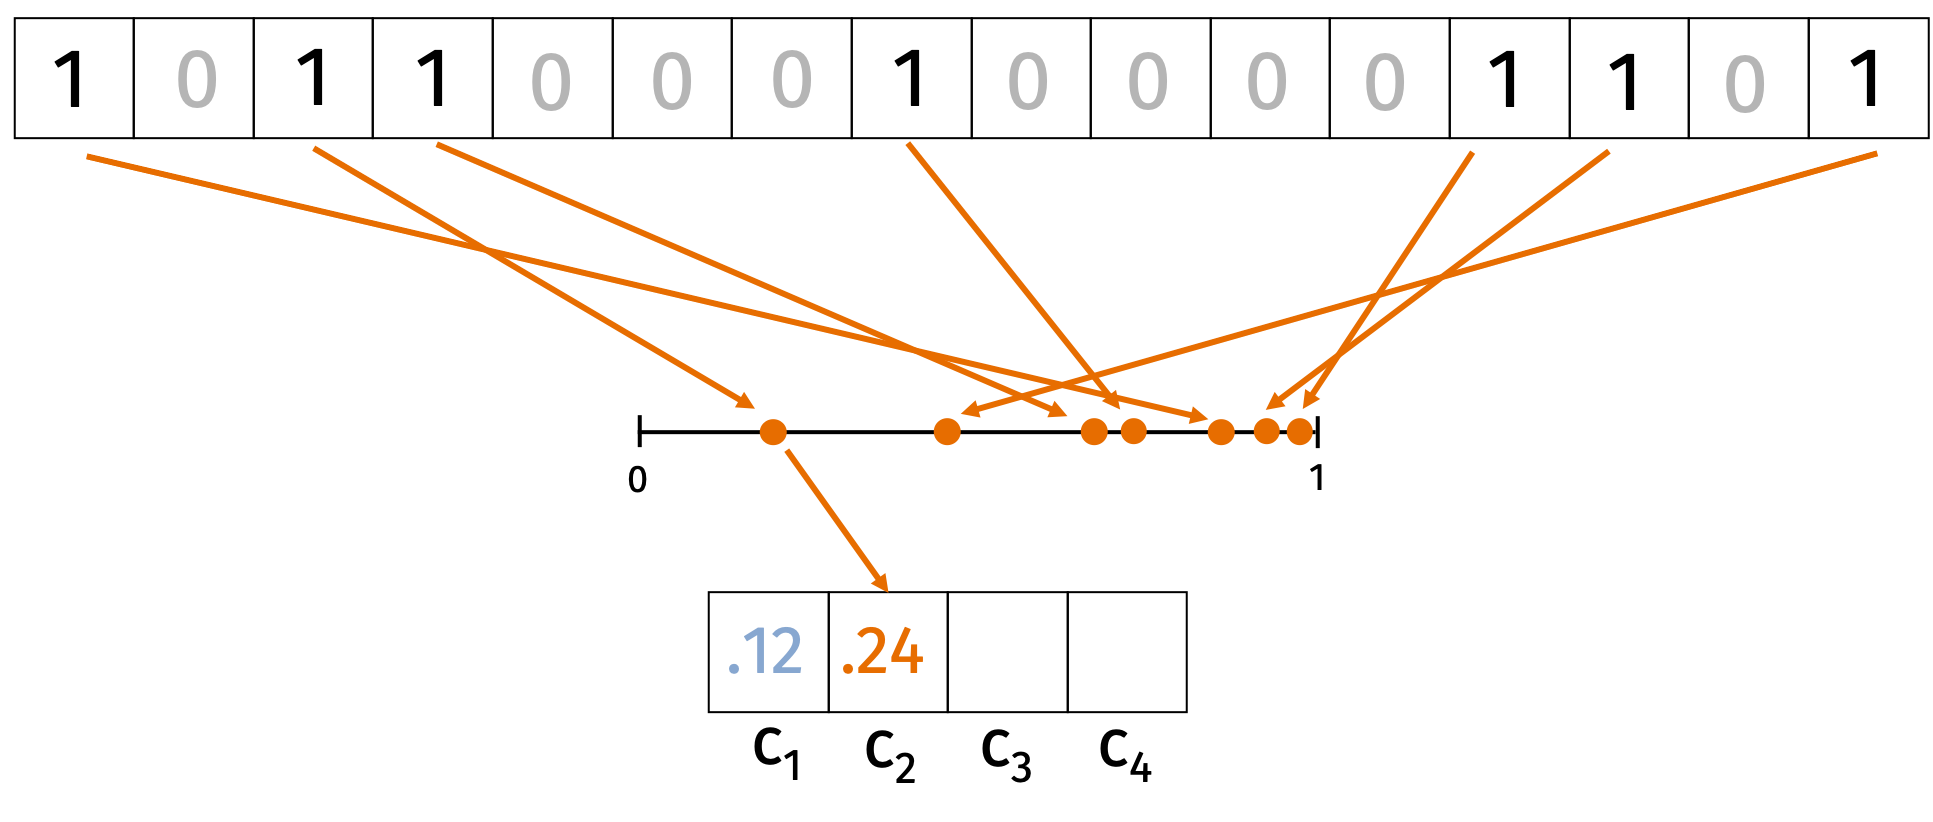
\includegraphics[width=\textwidth]{minHash2.png}	
	\end{center}
\end{frame}

\begin{frame}[t]
	\frametitle{minhash analysis}
	\textbf{Claim:} For all $i$, $\Pr[c_i(\bv{q}) = c_i(\bv{y})] = J(\bv{q},\bv{y}) = \frac{|\bv{q} \cap \bv{y}|}{|\bv{q} \cup \bv{y}|}$.
	\begin{center}
		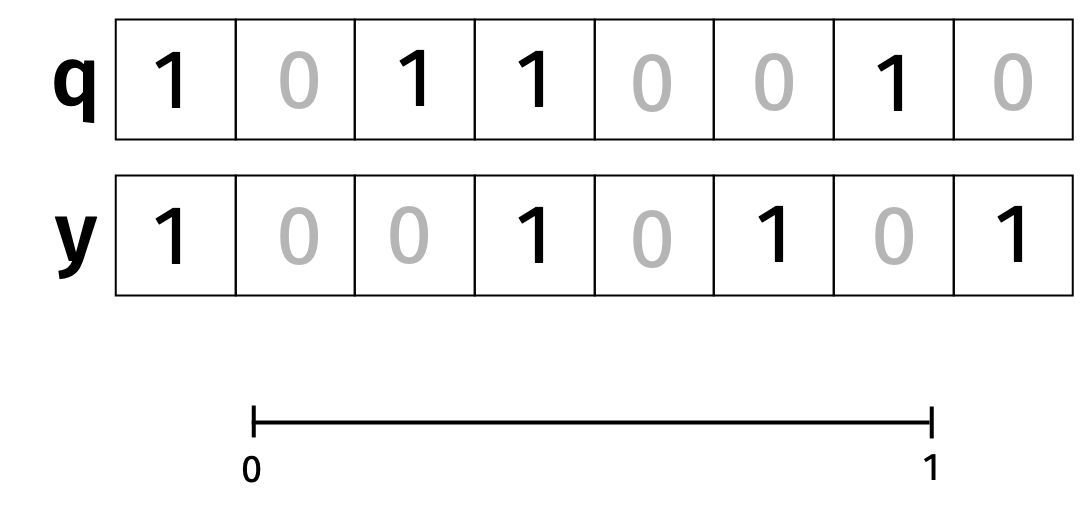
\includegraphics[width=.8\textwidth]{minHashSimple.png}
	\end{center}
	\textbf{Proof:} 
	
	1. For $c_i(\bv{q}) = c_i(\bv{y})$, we need that $\argmin_{i\in \bv{q}} h(i) = \argmin_{i\in \bv{y}} h(i)$.
\end{frame}

\begin{frame}[t]
	\frametitle{minhash analysis}
	\textbf{Claim:} $\Pr[c_i(\bv{q}) = c_i(\bv{y})] = J(\bv{q},\bv{y})$.	
	\begin{center}
		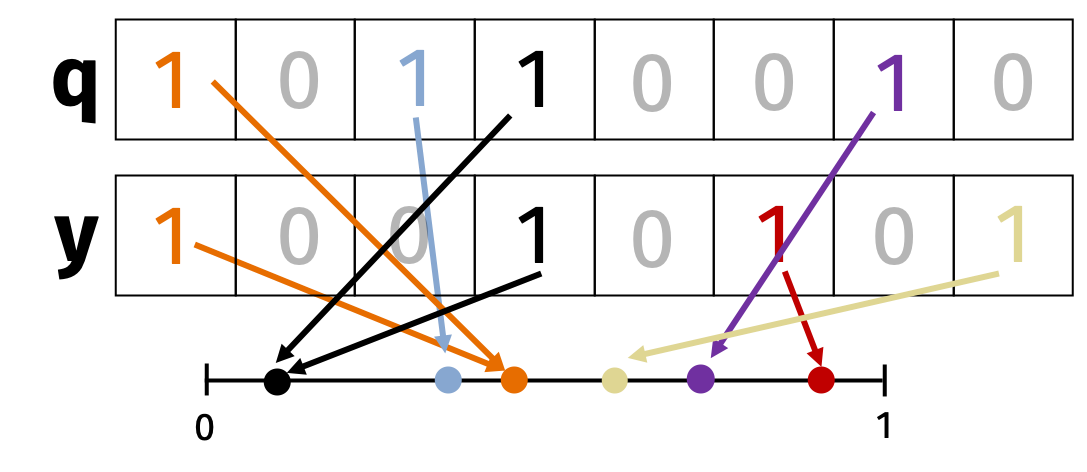
\includegraphics[width=.8\textwidth]{minhash_colored.png}
	\end{center}
	2. Every non-zero index in $\bv{q}\cup \bv{y}$ is equally likely to produce the lowest hash value.
	$c_i(\bv{q}) = c_i(\bv{y})$ only if this index is 1 in \emph{both} $\bv{q}$ and $\bv{y}$. There are $\bv{q}\cap \bv{y}$ such indices. So:
	\begin{align*}
		\Pr[c_i(\bv{q}) =c_i(\bv{y})]= \frac{|\bv{q}\cap \bv{y}|}{|\bv{q}\cup \bv{y}|}  = J(\bv{q},\bv{y})
	\end{align*}
\end{frame}


\begin{frame}
	\frametitle{minhash analysis}
	Let $J = J(\bv{q},\bv{y})$ denote the Jaccard similarity between $\bv{q}$ and $\bv{y}$. \vspace{1em}
	
	\textbf{Return:} $\tilde{J} = \frac{1}{k} \sum_{i=1}^k \mathbbm{1}[c_i(\bv{q}) = c_i(\bv{y})]$. 
	
	\textbf{Unbiased estimate for Jaccard similarity:}
	\begin{align*}
		\E \tilde{J} = \hspace{14em}
	\end{align*}
	
	\begin{center}
		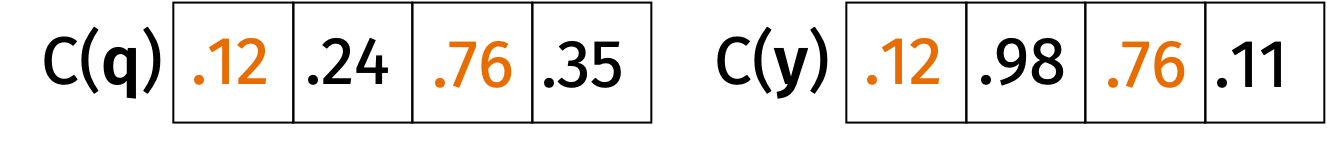
\includegraphics[width=.6\textwidth]{minHashCompare.png}
	\end{center}
	The more repetitions, the lower the variance. 
\end{frame}

\begin{frame}[t]
	\frametitle{minhash analysis}
	Let $J = J(\bv{q},\bv{y})$ denote the true Jaccard similarity.
	
	\textbf{Estimator:} $\tilde{J} = \frac{1}{k} \sum_{i=1}^k \mathbbm{1}[c_i(\bv{q}) = c_i(\bv{y})]$. 
	\begin{align*}
		\Var [\tilde{J}] =\hspace{16em}
	\end{align*}
	
	Plug into Chebyshev inequality. How large does $k$ need to be so that with probability $> 1 - \delta$, $|J-\tilde{J}| \leq \epsilon$?
\end{frame}

\begin{frame}
	\frametitle{minhash analysis}
	\textbf{Chebyshev inequality:} As long as $\alert{{k = O\left(\frac{1}{\epsilon^2\delta}\right)}}$, then with prob. $1-\delta$,
	\begin{align*}
		J(\bv{q}, \bv{y}) -\epsilon \leq \tilde{J}\left(C(\bv{q}),C(\bv{y})\right)   \leq J(\bv{q}, \bv{y}) + \epsilon. 
	\end{align*}
	\begin{center}
		And $\tilde{J}$ only takes $O(k)$ time to compute! \alert{\textbf{Independent}} of original fingerprint dimension $d$.
	\end{center}	
	
	Can be improved to $\log(1/\delta)$ dependence. Can anyone tell me how?
\end{frame}



\begin{frame}
	\frametitle{similarity sketching}
	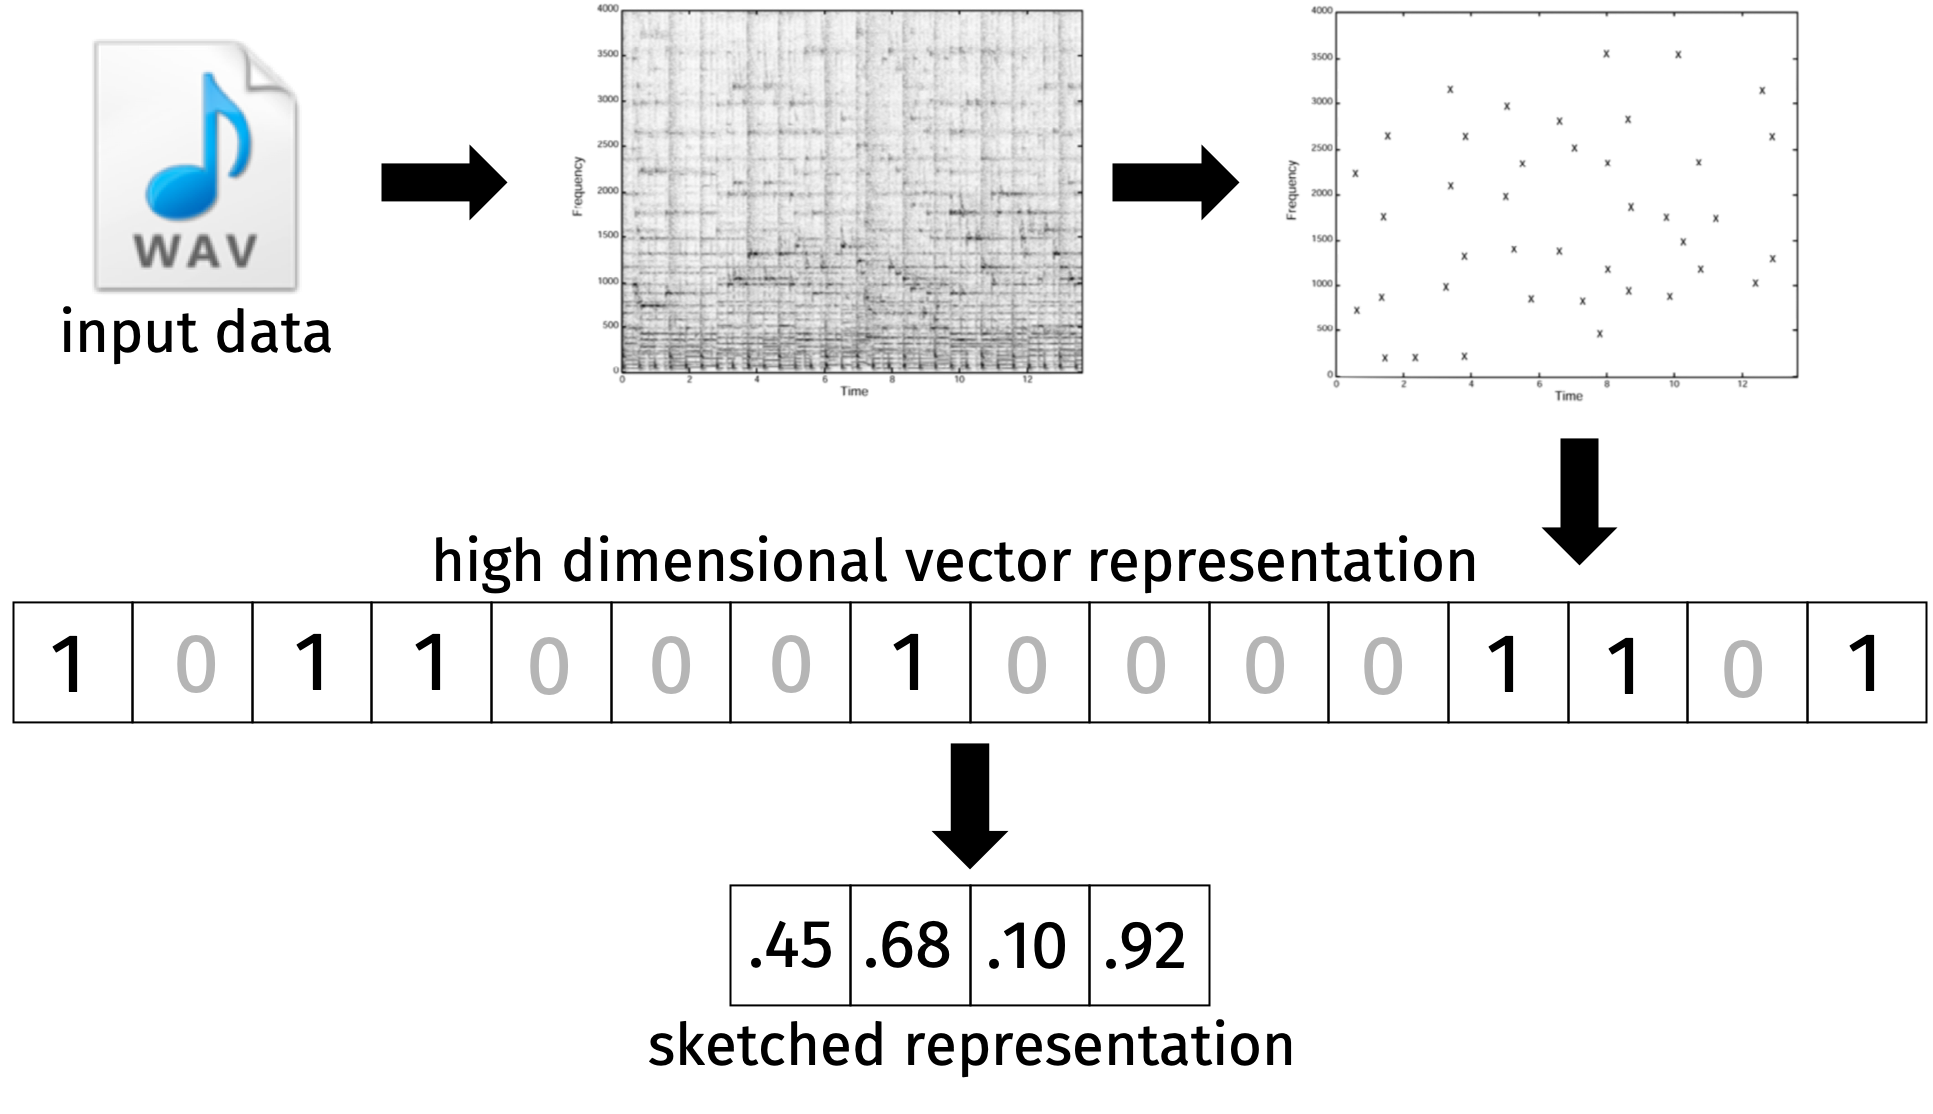
\includegraphics[width=\textwidth]{sketch_paradigm.png}
\end{frame}

\begin{frame}[standout]
	\begin{center}
		break
	\end{center}
\end{frame}

\begin{frame}
	\frametitle{near neighbor search}
	\textbf{Common goal:} Find all vectors in database $\bv{q}_1, \ldots, \bv{q}_n \in \R^d$ that are close to some input query vector $\bv{y}\in \R^d$. I.e. find all of $\bv{y}$'s ``nearest neighbors'' in the database.
	\begin{itemize}
		\item The Shazam problem.
		\item Audio + video search.
		\item Finding duplicate or near duplicate documents.
		\item Detecting seismic events.
	\end{itemize}

		\begin{center}
	\textbf{\alert{How does similarity sketching help in these applications?}}
		\end{center}
	\begin{itemize}
		\item Improves runtime of ``linear scan'' from $O(nd)$ to $O(nk)$.
		\item Improves space complexity from $O(nd)$ to $O(nk)$. This can be super important -- e.g. if it means the linear scan only accesses vectors in fast memory.
	\end{itemize}
\end{frame}

\begin{frame}
	\frametitle{beyond a linear scan}
	\begin{center}
		\textbf{New goal:} \emph{Sublinear} $o(n)$ time to find near neighbors. 
	\end{center}
\end{frame}

\begin{frame}
	\frametitle{beyond a linear scan}	
	This problem can already be solved for a small number of dimensions using space partitioning approaches (e.g. kd-tree).
	
	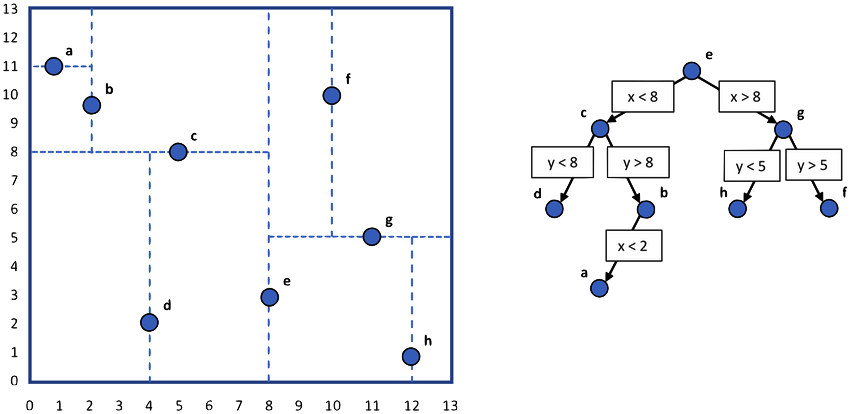
\includegraphics[height=.4\textheight]{kdtree.png}	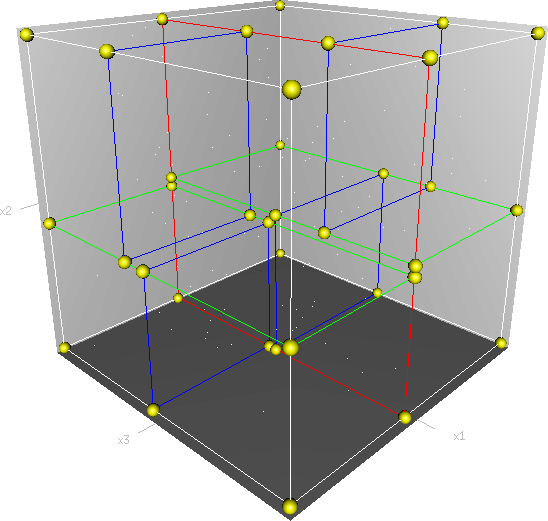
\includegraphics[height=.4\textheight]{3dtree.png}
	
	Runtime is roughly $O(d\cdot \min(n,2^d))$, which is only sublinear for $d = o(\log n)$.

\end{frame}

\begin{frame}
	\frametitle{high dimensional near neighbor search}	
	Only been attacked much more recently:
	\begin{itemize}
		\item \textbf{\alert{Locality-sensitive hashing [Indyk, Motwani, 1998]}}
		\item Spectral hashing [Weiss, Torralba, and Fergus, 2008]
		\item Vector quantization [J\'{e}gou, Douze, Schmid, 2009]
	\end{itemize}

\textbf{Key Insight of LSH:} Trade worse space-complexity for better time-complexity. I.e. typically use more than $O(n)$ space.
\end{frame}

\begin{frame}
	\frametitle{locality sensitive hash functions}
	Let $h: \R^d \rightarrow \{1, \ldots, m\}$ be a random hash function. 
	
	We call $h$ \emph{locality sensitive} for similarity function $s(\bv{q},\bv{y})$ if $\Pr\left[h(\bv{q}) == h(\bv{y})\right]$ is:
	\begin{itemize}
		\item Higher when $\bv{q}$ and $\bv{y}$ are more similar, i.e. $s(\bv{q},\bv{y})$ is higher.
		\item Lower when $\bv{q}$ and $\bv{y}$ are more dissimilar, i.e. $s(\bv{q},\bv{y})$ is lower. 
	\end{itemize}
\begin{center}
	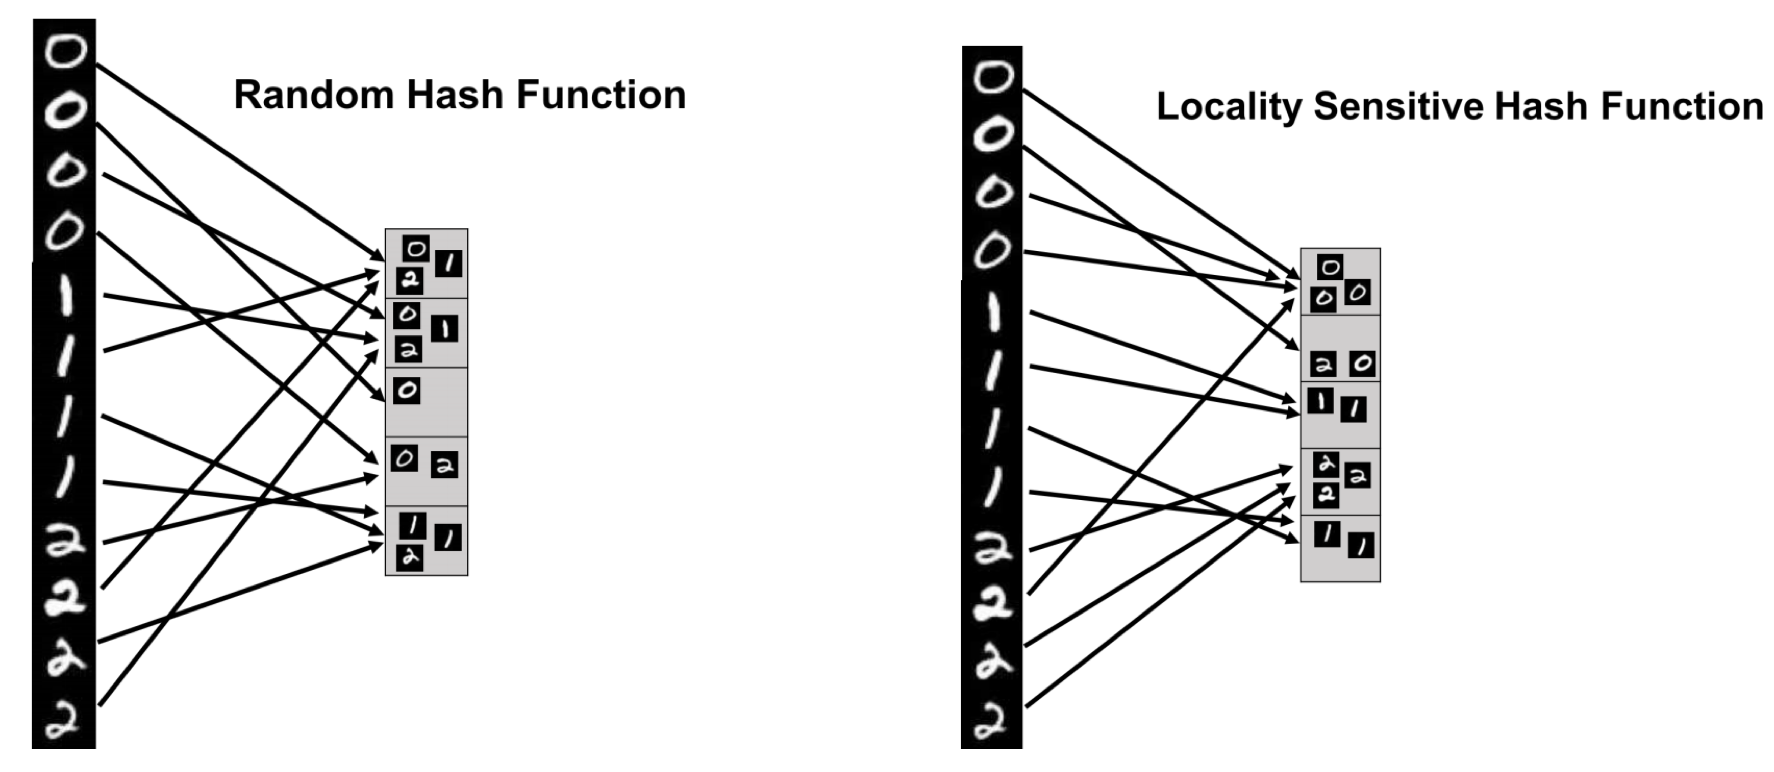
\includegraphics[width=.9\textwidth]{cam_lsh.png}
\end{center}
\end{frame}

\begin{frame}
	\frametitle{locality sensitive hash functions}
	LSH for $s(\bv{q},\bv{y})$  equal to Jaccard similarity:
	\begin{itemize}
		\item Let $c: \{0,1\}^d \rightarrow [0,1]$ be a single instantiation of MinHash.
		\item Let $g: [0,1] \rightarrow \{1, \ldots, m\}$ be a uniform random hash function.
		\item Let $h(\bv{q}) = g(c(\bv{q})).$
	\end{itemize}
\begin{center}
	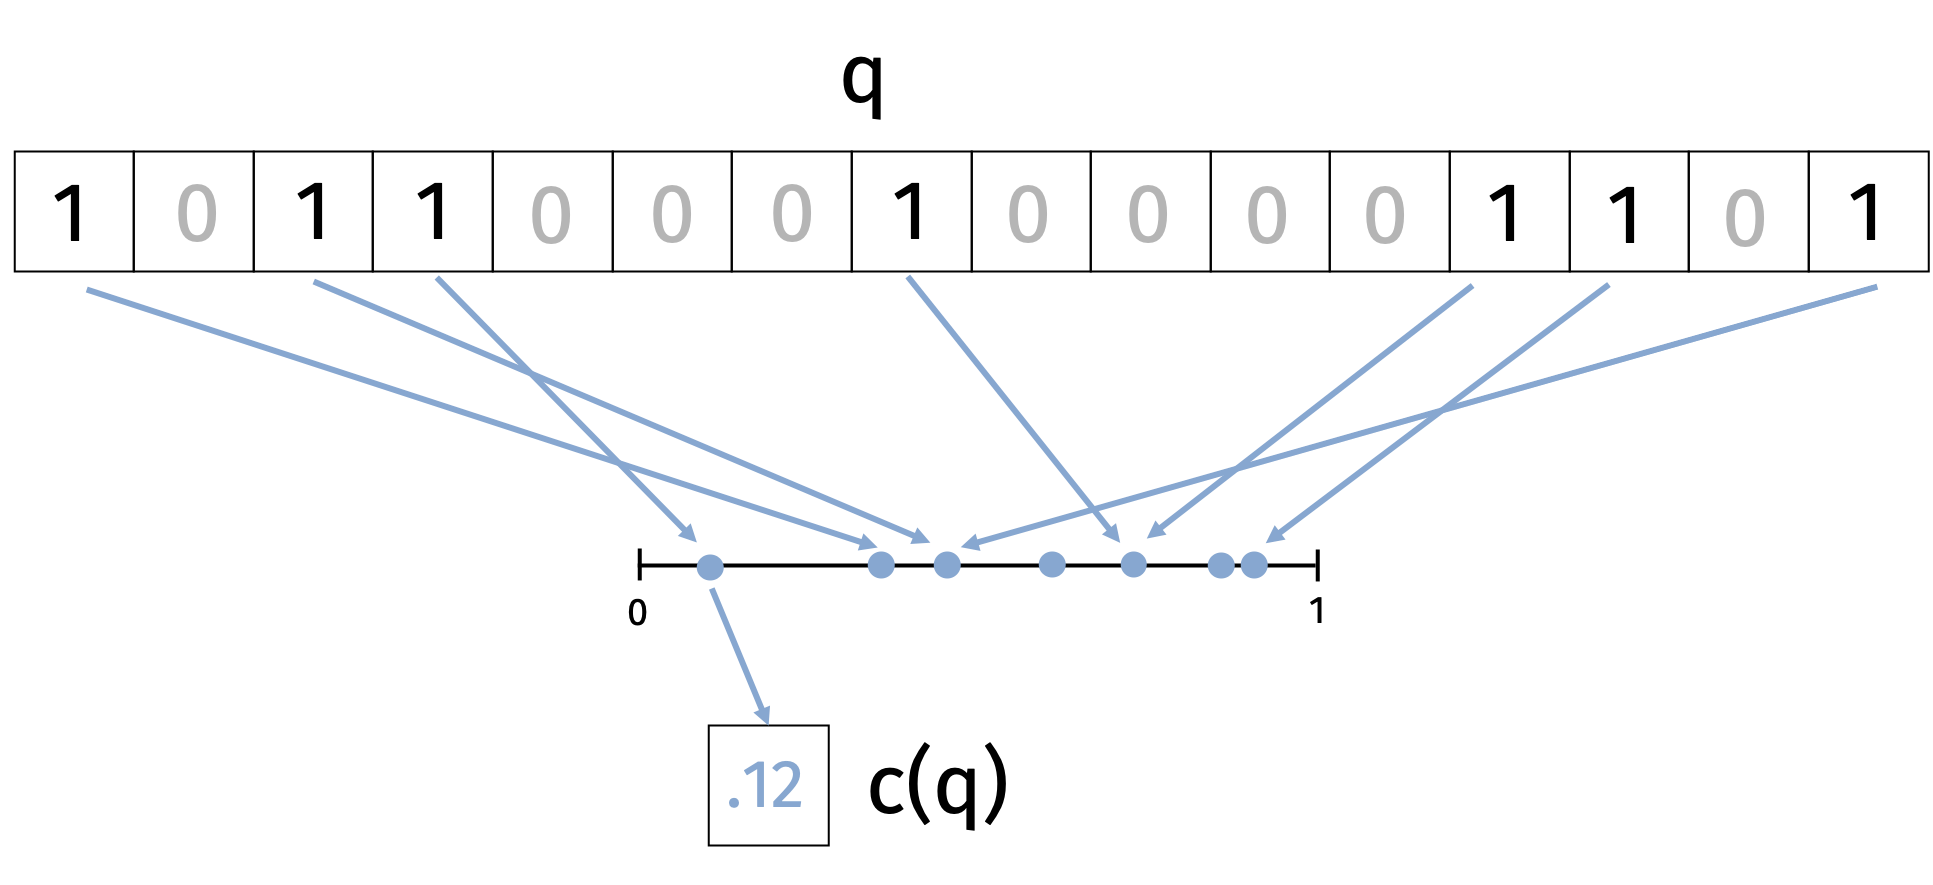
\includegraphics[width=.7\textwidth]{single_min_hash.png}
\end{center}

\end{frame}

\begin{frame}
	\frametitle{locality sensitive hash functions}
	LSH for Jaccard similarity:
	\begin{itemize}
		\item Let $c: \{0,1\}^d \rightarrow [0,1]$ be a single instantiation of MinHash.
		\item Let $g: [0,1] \rightarrow \{1, \ldots, m\}$ be a uniform random hash function.
		\item Let $h(\bv{x}) = g(c(\bv{x})).$
	\end{itemize}
		If $J(\bv{q},\bv{y}) = v$, 
		\begin{align*}
			\Pr\left[h(\bv{q}) == h(\bv{y})\right] = \hspace{15em}
		\end{align*}
\end{frame}

\begin{frame}
	\frametitle{near neighbor search}
	\begin{center}
	Basic approach for near neighbor search in a database.
	\end{center}
		\textbf{Pre-processing:}
	\begin{itemize}
		\item Select random LSH function $h: \{0,1\}^d \rightarrow 1,\ldots, m$.
		\item Create table $T$ with $m = O(n)$ slots.\footnote{Enough to make the $O(1/m)$ term negligible.}
		\item For $i = 1,\ldots, n$, insert $\bv{q}_i$ into $T(h(\bv{q}_i))$.
	\end{itemize}
	\textbf{Query:}
	\begin{itemize}
		\item Want to find near neighbors of input $\bv{y}\in\{0,1\}^d$.
		\item Linear scan through all vectors $\bv{q}\in T(h(\bv{y}))$ and return any that are close to $\bv{y}$. Time required is $O(d\cdot |T(h(\bv{y})|)$.
	\end{itemize}
\vspace{1em}
\end{frame}

\begin{frame}
	\frametitle{near neighbor search}
	\begin{center}
		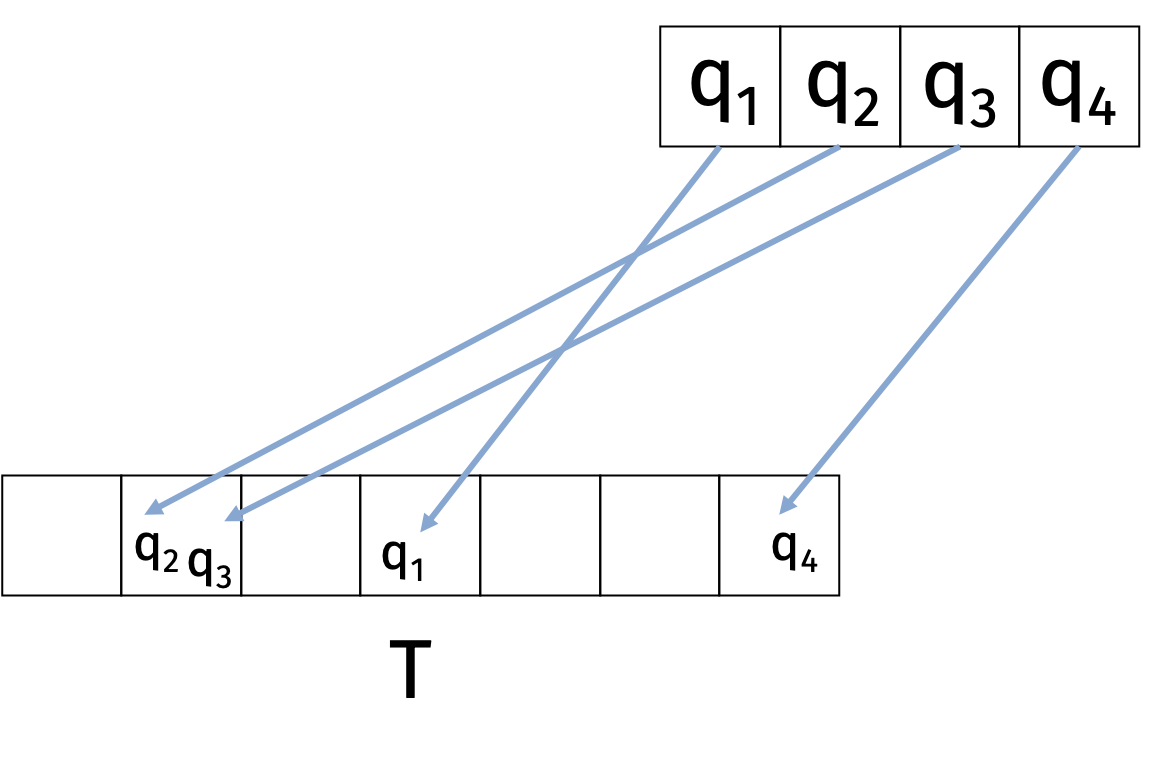
\includegraphics[width=.8\textwidth]{basicScheme.png}
	\end{center}
\end{frame}

\begin{frame}
	\frametitle{near neighbor search}
	\textbf{Two main considerations:}
	\begin{itemize}
		\item \textbf{False Negative Rate}: What's the probability we do not find a vector that \emph{is close} to $\bv{y}$?
		\item \textbf{False Positive Rate}: What's the probability that a vector in $T(h(\bv{y}))$ \emph{is not close} to $\bv{y}$?
	\end{itemize}

A higher false negative rate means we miss near neighbors.

A higher false positive rate means increased runtime -- we need to compute $J(\bv{q},\bv{y})$ for every $\bv{q}\in T(h(\bv{y}))$ to check if it's actually close to $\bv{y}$.

\textbf{Note:} The meaning of ``close'' and ``not close'' is application dependent. E.g. we might specify that we want to find anything with Jaccard similarity $> .4$, but not with Jaccard similarity $< .2$. 
\end{frame}

\begin{frame}
	\frametitle{reducing false negative rate}	
	Suppose the nearest database point $\bv{q}$ has $J(\bv{y},\bv{q}) = .4$.
	\begin{center}
	\textbf{\alert{What's the probability we do not find $\bv{q}$?}}
	\end{center}
\end{frame}

\begin{frame}
	\frametitle{reducing false negative rate}
	\begin{center}
		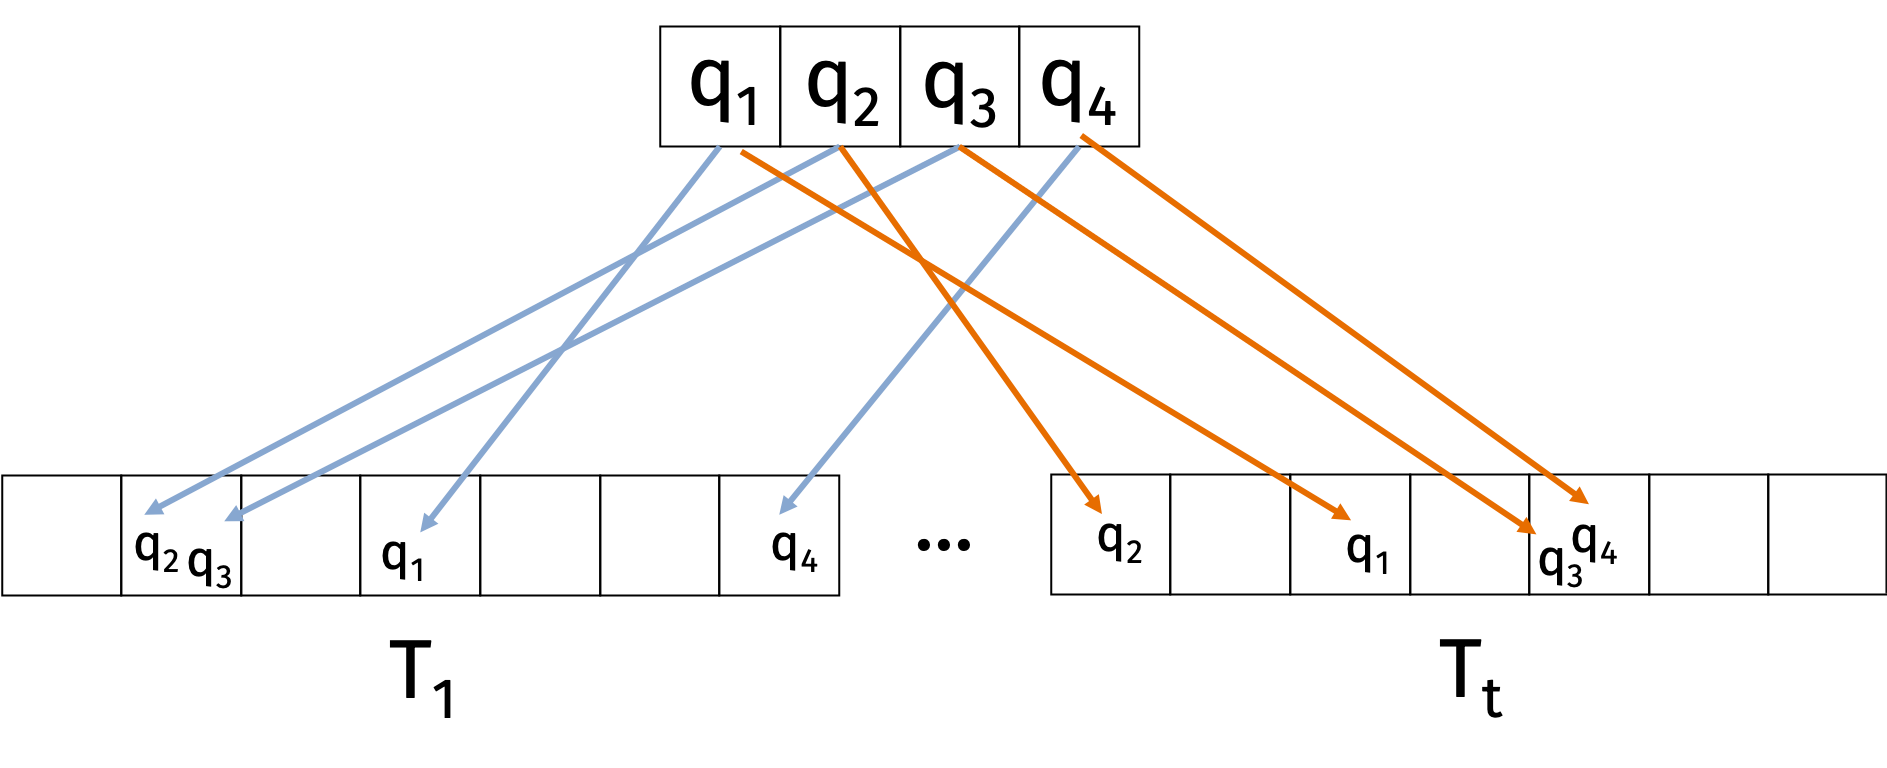
\includegraphics[width=.8\textwidth]{many_tables.png}
	\end{center}
	\textbf{Pre-processing:}
	\begin{itemize}
		\item Select $t$ independent LSH's $h_1, \ldots, h_t: \{0,1\}^d \rightarrow 1,\ldots, m$.
		\item Create tables $T_1, \ldots, T_t$, each with $m$ slots. 
		\item For $i = 1,\ldots, n$, $j = 1,\ldots, t$, 
		\begin{itemize}
			\item Insert $\bv{q}_i$ into $T_j(h_j(\bv{q}_i))$.
		\end{itemize}
	\end{itemize}
\end{frame}

\begin{frame}[t]
	\frametitle{reducing false negative rate}
	\textbf{Query:}
	\begin{itemize}
		\item Want to find near neighbors of input $\bv{y}\in\{0,1\}^d$.
		\item Linear scan through all vectors in $T_1(h_1(\bv{y}))\cup T_2(h_2(\bv{y}))\cup \ldots, T_t(h_t(\bv{y}))$.
	\end{itemize}

\vspace{2em}
	Suppose the nearest database point $\bv{q}$ has $J(\bv{y},\bv{q}) = .4$.
	\begin{center}
		\textbf{\alert{What's the probability we find $\bv{q}$?}}
	\end{center}
	
	\vskip0pt plus 1filll
	\hspace{-1em}\scriptsize($10$, $99\%$)
\end{frame}

\begin{frame}[t]
	\frametitle{what happens to false positives?}
	Suppose there is some other database point $\bv{z}$ with $J(\bv{y},\bv{z}) = .2$. 
	
	What is the probability we will need to compute $J(\bv{z},\bv{y})$ in our hashing scheme with one table? I.e. the probability that $\bv{y}$ hashes into at least one bucket containing $\bv{z}$. 
	
	\vspace{4em}
	{\textbf{\alert{In the new scheme with $t=10$ tables?}}}
	
	\vskip0pt plus 1filll
	\hspace{-1em}\scriptsize($89\%$)
\end{frame}

\begin{frame}[t]
	\frametitle{reducing false positives}
	\small
	\vspace{-.5em}
	\begin{center}
	\textbf{Change our locality sensitive hash function}.
	\vspace{-.5em}
	\end{center}
	\emph{Tunable} LSH for Jaccard similarity:
	\vspace{-.5em}
	\begin{itemize}
		\item Choose parameter $r \in \mathbb{Z}^+$.
		\item Let $c_1, \ldots, c_r: \{0,1\}^d \rightarrow [0,1]$ be random MinHash.
		\item Let $g: [0,1]^r \rightarrow \{1, \ldots, m\}$ be a uniform random hash function.
		\item Let $h(\bv{x}) = g(c_1(\bv{x}), \ldots, c_r(\bv{x})).$
	\end{itemize}
\vspace{-1em}
	\begin{center}
			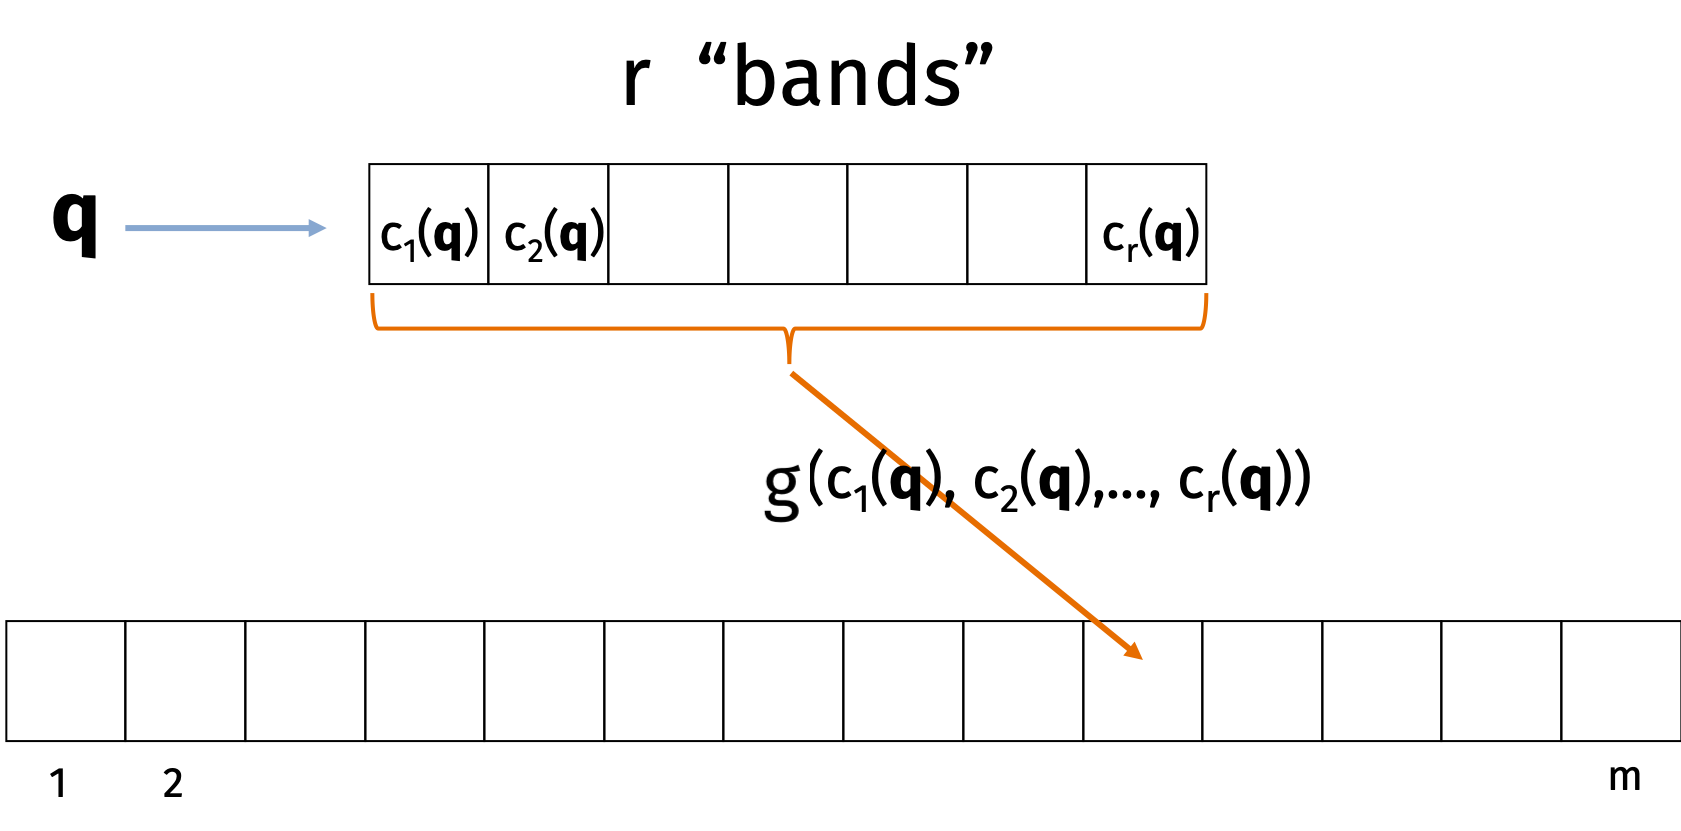
\includegraphics[width=.8\textwidth]{banded_hash.png}
	\end{center}


\end{frame}

\begin{frame}[t]
	\frametitle{reducing false positives}
	\small
	\emph{Tunable} LSH for Jaccard similarity:
	\begin{itemize}
		\item Choose parameter $r \in \mathbb{Z}^+$.
		\item Let $c_1, \ldots, c_r: \{0,1\}^d \rightarrow [0,1]$ be random MinHash.
		\item Let $g: [0,1]^r \rightarrow \{1, \ldots, m\}$ be a uniform random hash function.
		\item Let $h(\bv{x}) = g(c_1(\bv{x}), \ldots, c_r(\bv{x})).$
	\end{itemize}
	
	If $J(\bv{q},\bv{y}) = v$, then $\Pr\left[h(\bv{q}) == h(\bv{y})\right] = $
	
\end{frame}

\begin{frame}[t]
	\frametitle{tunable lsh}
	\begin{center}
		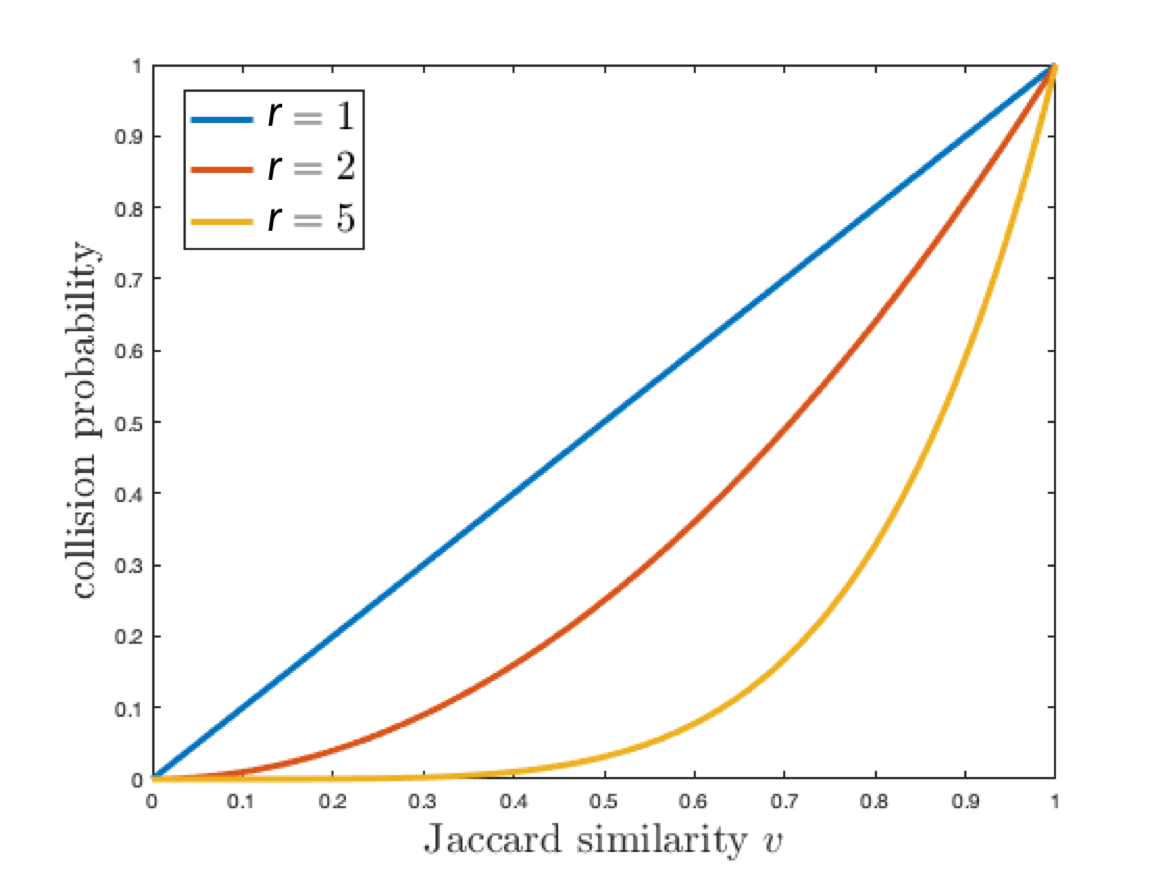
\includegraphics[width=.8\textwidth]{tuning_minhash.png}
	\end{center}
\end{frame}

\begin{frame}[t]
	\frametitle{tunable lsh}
	Full LSH cheme has two parameters to tune:
	\begin{center}
		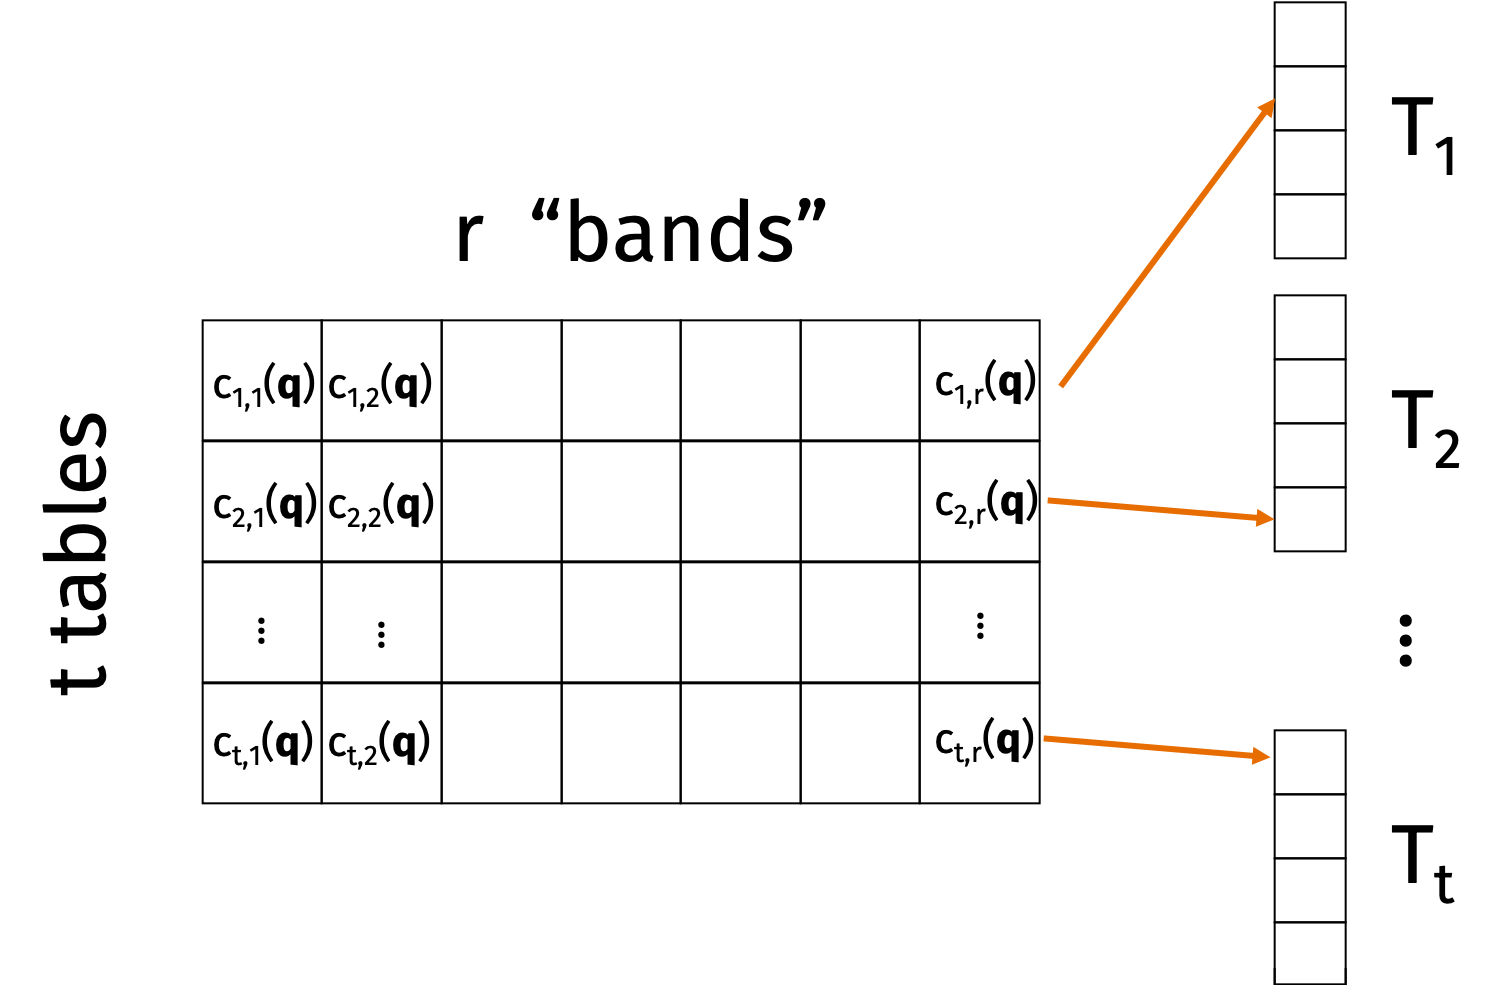
\includegraphics[width=.8\textwidth]{full_scheme.png}
	\end{center}
\end{frame}

\begin{frame}[t]
	\frametitle{tunable lsh}
	Effect of \textbf{increasing number of tables} $t$ on:
	\begin{center}
		False Negatives \hspace{6em} False Positives
	\end{center}
\vspace{4em}
	Effect of \textbf{increasing number of bands} $r$ on:
\begin{center}
	False Negatives \hspace{6em} False Positives
\end{center}
\end{frame}

%\begin{frame}
%	\frametitle{some examples}
%	Choose tables $t$ large enough so false negative rate to $1\%$.
%	\begin{center}
%		\alert{\textbf{Parameter:} $\mathbf{r = 1}$.}
%	\end{center}
%	Chance we find $\bv{q}$ with $J(\bv{y},\bv{q}) = .8$:
%	\vspace{5em}
%	
%	Chance we need to check $\bv{z}$ with $J(\bv{y},\bv{z}) = .4$:
%\end{frame}
%
%\begin{frame}
%	\frametitle{some examples}
%	Choose tables $t$ large enough so false negative rate to $1\%$.
%	\begin{center}
%		\alert{\textbf{Parameter:} $\mathbf{r = 2}$.}
%	\end{center}
%	Chance we find $\bv{q}$ with $J(\bv{y},\bv{q}) = .8$:
%	\vspace{5em}
%	
%	Chance we need to check $\bv{z}$ with $J(\bv{y},\bv{z}) = .4$:
%\end{frame}
%
%\begin{frame}
%	\frametitle{some examples}
%	Choose tables $t$ large enough so false negative rate to $1\%$.
%	\begin{center}
%		\alert{\textbf{Parameter:} $\mathbf{r = 5}$.}
%	\end{center}
%	Chance we find $\bv{q}$ with $J(\bv{y},\bv{q}) = .8$:
%	\vspace{5em}
%	
%	Chance we need to check $\bv{z}$ with $J(\bv{y},\bv{z}) = .4$:
%\end{frame}

\begin{frame}
	\frametitle{$s$-curve tuning}
	Probability we check $\bv{q}$ when querying $\bv{y}$ if $J(\bv{q},\bv{y}) = v$:
	\begin{align*}
%	\approx 	1 - (1 - v^r)^t
	\end{align*}
	\begin{center}
		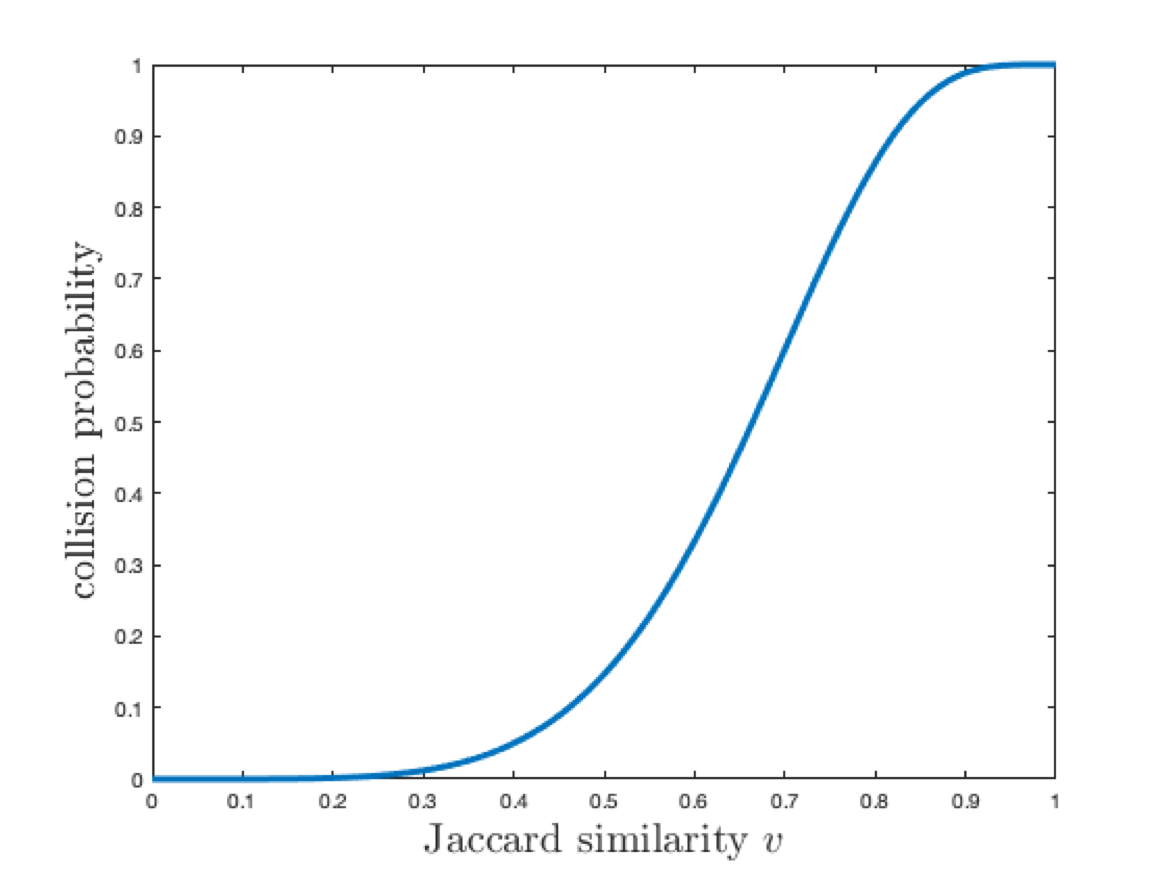
\includegraphics[width=.6\textwidth]{scurve_5_5.png}
		
		$r = 5, t = 5$
	\end{center}
\end{frame}

\begin{frame}
	\frametitle{$s$-curve tuning}
	Probability we check $\bv{q}$ when querying $\bv{y}$ if $J(\bv{q},\bv{y}) = v$:
	\begin{align*}
	\approx 1 - (1 - v^r)^t
	\end{align*}
	\begin{center}
		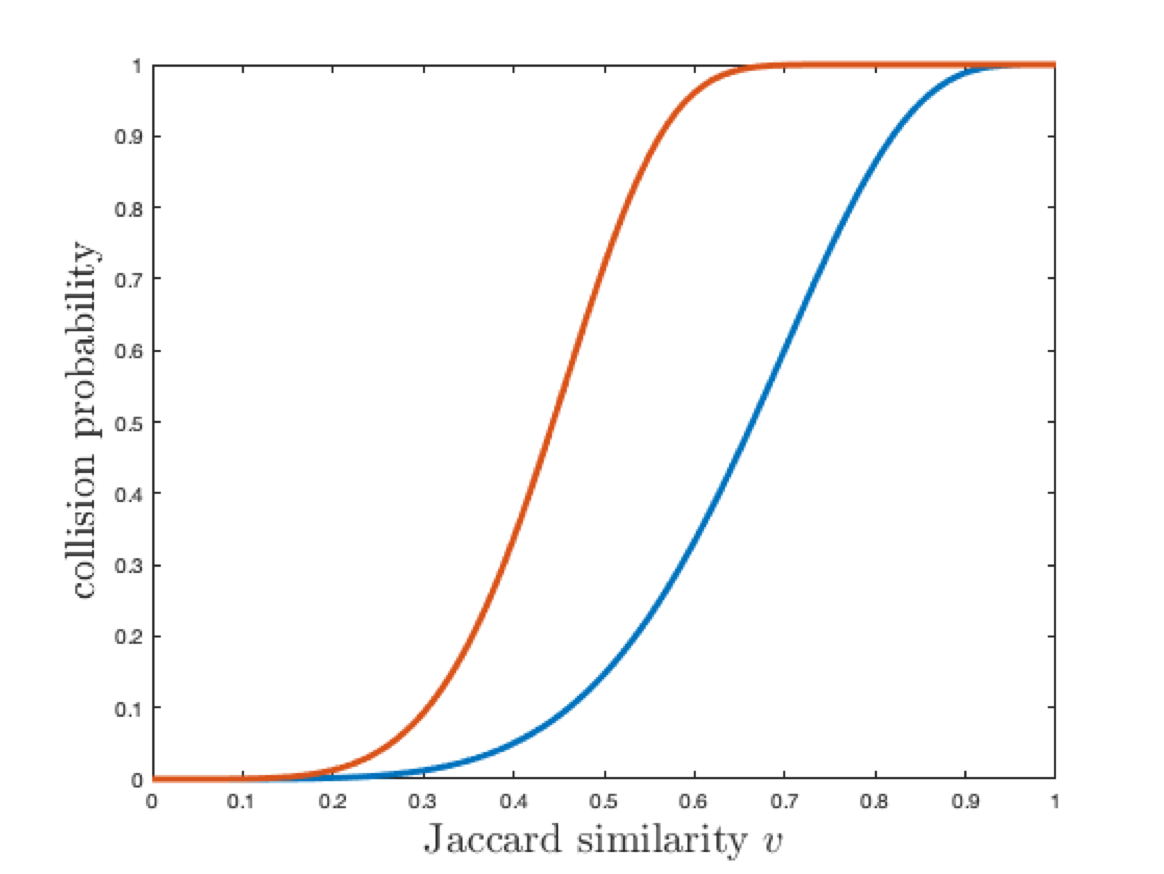
\includegraphics[width=.6\textwidth]{scurve_5_40.png}
		
		$r = 5, t = 40$
	\end{center}
\end{frame}

\begin{frame}
	\frametitle{$s$-curve tuning}
	Probability we check $\bv{q}$ when querying $\bv{y}$ if $J(\bv{q},\bv{y}) = v$:
	\begin{align*}
	\approx 1 - (1 - v^r)^t 
	\end{align*}
	\begin{center}
		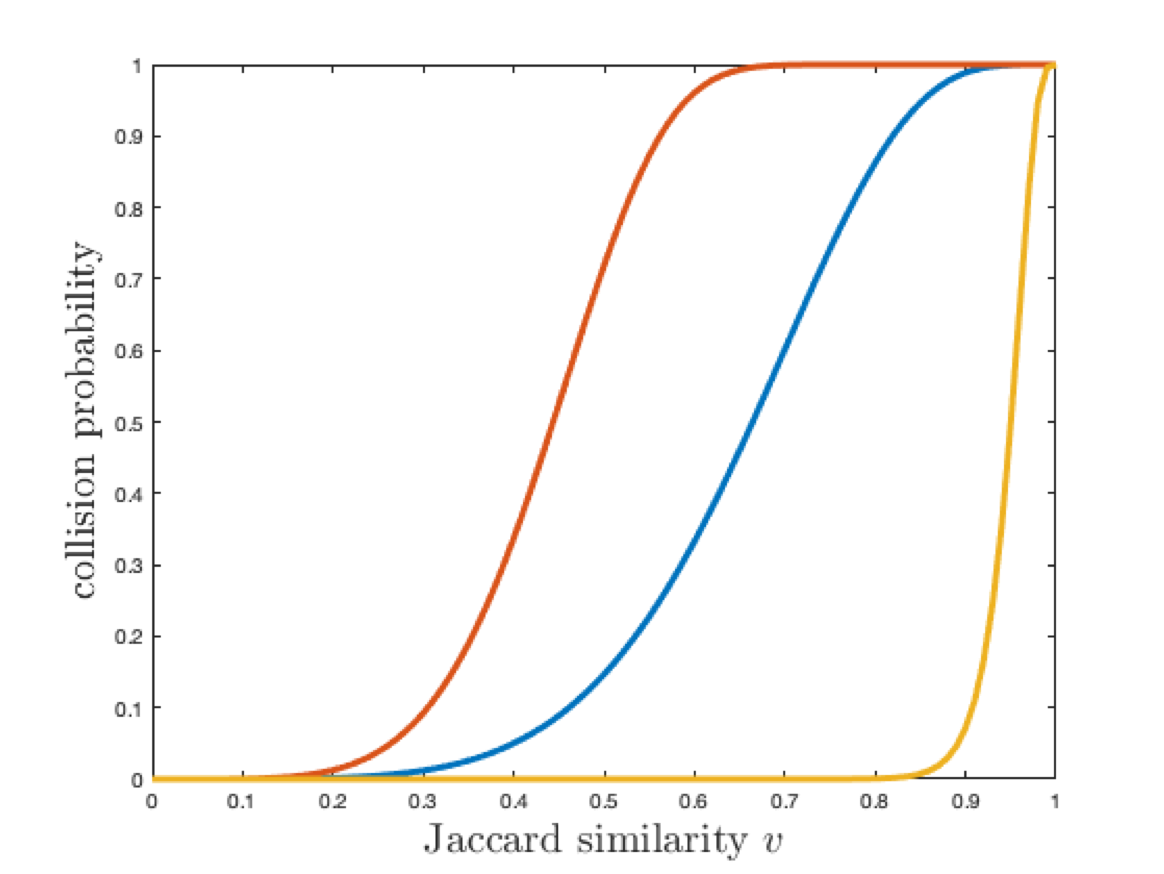
\includegraphics[width=.6\textwidth]{scurve_40_5.png}
		
		$r = 40, t = 5$
	\end{center}
\end{frame}

\begin{frame}
	\frametitle{$s$-curve tuning}
	Probability we check $\bv{q}$ when querying $\bv{y}$ if $J(\bv{q},\bv{y}) = v$:
	\begin{align*}
	1 - (1 - v^r)^t
	\end{align*}
	\begin{center}
		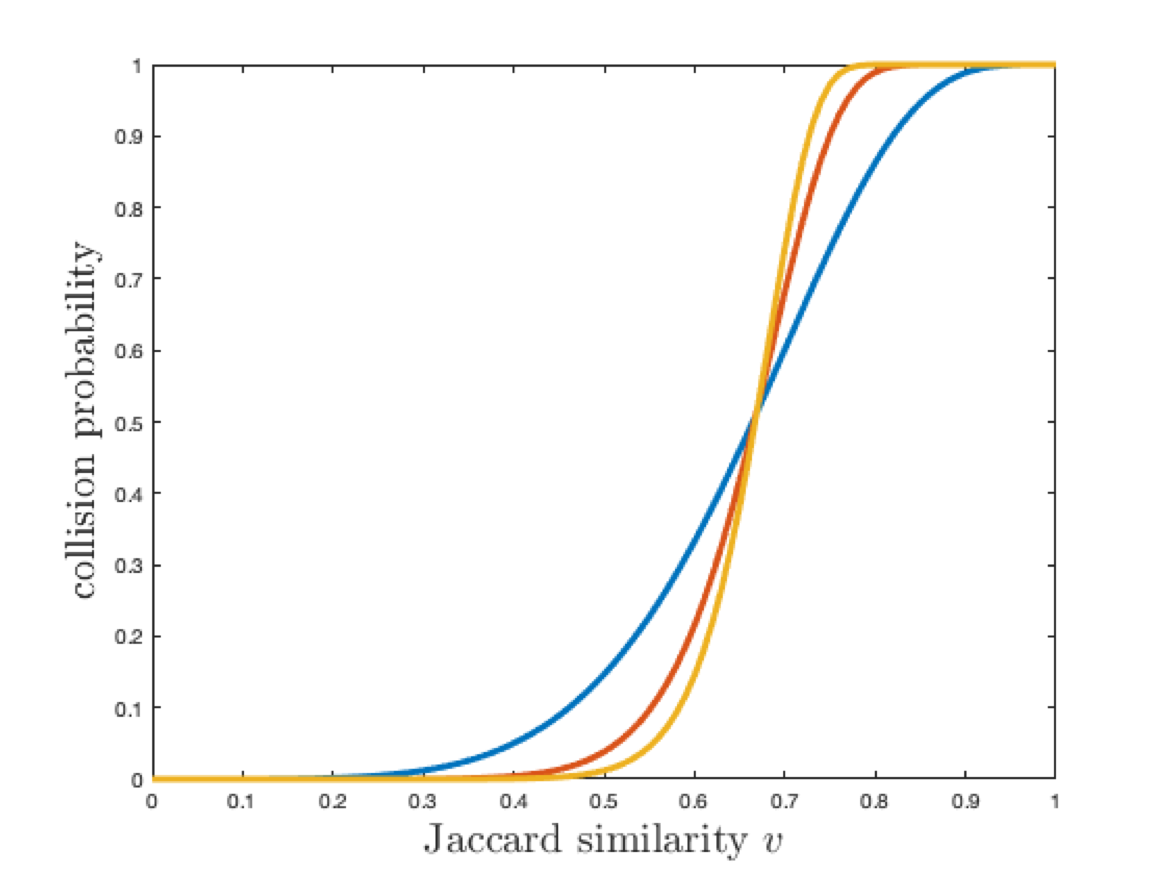
\includegraphics[width=.6\textwidth]{scurve_centered.png}
		
		Increasing both $r$ and $t$ gives a steeper curve. 
		
		\alert{\textbf{Better for search, but worse space complexity}.}
	\end{center}
\end{frame}

\begin{frame}
	\frametitle{fixed threshold}
	\small
	\textbf{Use Case 1:} Fixed threshold.
	\begin{itemize}
		\item Shazam wants to find match to audio clip $\bv{y}$ in a database of 10 million  clips.
		\item There are 10 \emph{true matches} with $J(\bv{y},\bv{q}) > .9$.
		\item There are 10,000 \emph{near matches} with $J(\bv{y},\bv{q}) \in [.7,.9]$.
		\item All other items have $J(\bv{y},\bv{q}) < .7$.
	\end{itemize}
	With $r = 25$ and $t = 40$, 
	\begin{itemize}
		\item Hit probability for $J(\bv{y},\bv{q}) > .9$ is $\gtrsim 1 - (1 - .9^{25})^{40} = .95$
		\item Hit probability for $J(\bv{y},\bv{q}) \in [.7,.9]$ is $\lesssim 1 - (1 - .9^{25})^{40} = .95$
		\item Hit probability for $J(\bv{y},\bv{q}) < .7$ is $\lesssim 1 - (1 - .7^{25})^{40} = .005$
	\end{itemize}
	\textbf{Upper bound on total number of items checked:} 
	\begin{align*}
	10 + .95 \cdot 10,000 + .005 \cdot 9,989,990 \alert{\approx 60,000 \ll 10,000,000}.
	\end{align*}  
\end{frame}

\begin{frame}
	\frametitle{fixed threshold}
	\begin{center}
	Space complexity: 40 hash tables \alert{$\approx 40\cdot O(n)$}. 
	
	\textbf{Directly trade space for fast search.}
	\end{center}
\end{frame}

\begin{frame}
	\frametitle{fixed threshold r}
	\begin{center}
	\textbf{Near Neighbor Search Problem}
\end{center}

	Concrete worst case result:
	\begin{theorem}[Indyk, Motwani, 1998]
		If there exists some $q$ with $\|\bv{q} - \bv{y}\|_0 \leq R$, return a vector $\tilde{\bv{q}}$ with $\|\tilde{\bv{q}} - \bv{y}\|_0 \leq C\cdot R$ in:
		\begin{itemize}
			\item Time: $O\left(n^{1/C}\right)$.
			\item Space: $O\left(n^{1 + 1/C}\right)$. 
		\end{itemize}
	\end{theorem}
	$\|\bv{q} - \bv{y}\|_0 = $ ``hamming distance" = number of elements that differ between $\bv{q}$ and $\bv{y}$. 
\end{frame}

\begin{frame}
	\frametitle{approximate nearest neighbor search}
		\begin{theorem}[Indyk, Motwani, 1998]
		Let $q$ be the closest database vector to $\bv{y}$. Return a vector $\tilde{\bv{q}}$ with $\|\tilde{\bv{q}} - \bv{y}\|_0 \leq C\cdot \|{\bv{q}} - \bv{y}\|_0$ in:
		\begin{itemize}
			\item Time: $\tilde{O}\left(n^{1/C}\right)$.
			\item Space: $\tilde{O}\left(n^{1 + 1/C}\right)$. 
		\end{itemize}
	\end{theorem}
\end{frame}

\begin{frame}
	\frametitle{other lsh functions}
	\begin{center}
	Good locality sensitive hash functions exists for other similarity measures.
	\end{center}
	\textbf{Cosine similarity $\cos\left(\theta(\bv{x},\bv{y})\right) = \frac{\langle \bv{x},\bv{y}\rangle}{\|\bv{x}\|_2\|\bv{y}\|_2}$:}
	\begin{center}
		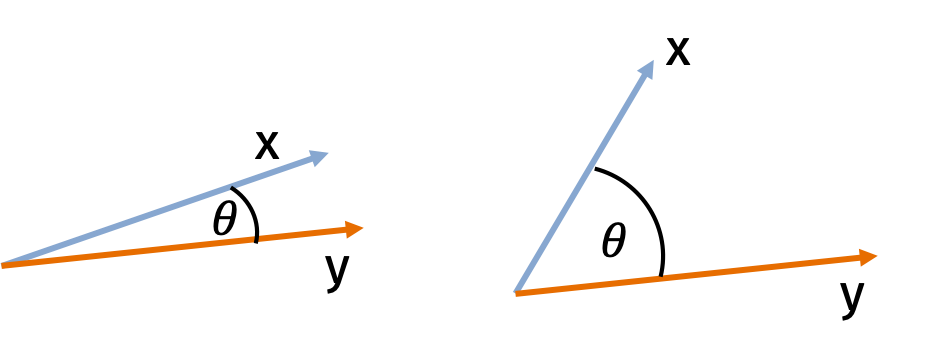
\includegraphics[width=.7\textwidth]{cos_sim.png}
		
		$-1 \leq \cos\left(\theta(\bv{x},\bv{y})\right) \leq 1$.
	\end{center}
\end{frame}

\begin{frame}
	\frametitle{cosine similarity}
	\begin{center}
		Cosine similarity is natural ``inverse" for Euclidean distance.
	\end{center}
		\textbf{Euclidean distance $\|\bv{x} - \bv{y}\|_2^2$:}
		\begin{itemize}
			\item Suppose for simplicity that $\|\bv{x}\|_2^2 = \|\bv{y}\|_2^2 = 1$.
		\end{itemize}
\end{frame}

\begin{frame}
	\frametitle{simhash}
	Locality sensitive hash for \textbf{cosine similarity}:
	\begin{itemize}
		\item Let $\bv{g} \in \R^d$ be randomly chosen with each entry $\mathcal{N}(0,1)$. 
		\item Let $f: \{-1,1\} \rightarrow \{1,\ldots, m\}$ be a uniformly random hash function. 
		\item $h: \R^d \rightarrow \{1,\ldots, m\}$ is definied $h(\bv{x}) = f\left(\sign(\langle \bv{g}, \bv{x} \rangle)\right)$.
	\end{itemize}
	\begin{center}
		\alert{\textbf{
				\large
				If $\cos(\theta(\bv{x},\bv{y})) = v$, what is $\Pr[h(\bv{x}) == h(\bv{y})]$?
		}}
	\end{center}
\end{frame}


%\begin{frame}
%	\frametitle{simhash}
%	\begin{center}
%		\textbf{Inspired by Johnson-Lindenstrauss sketching}
%		
%		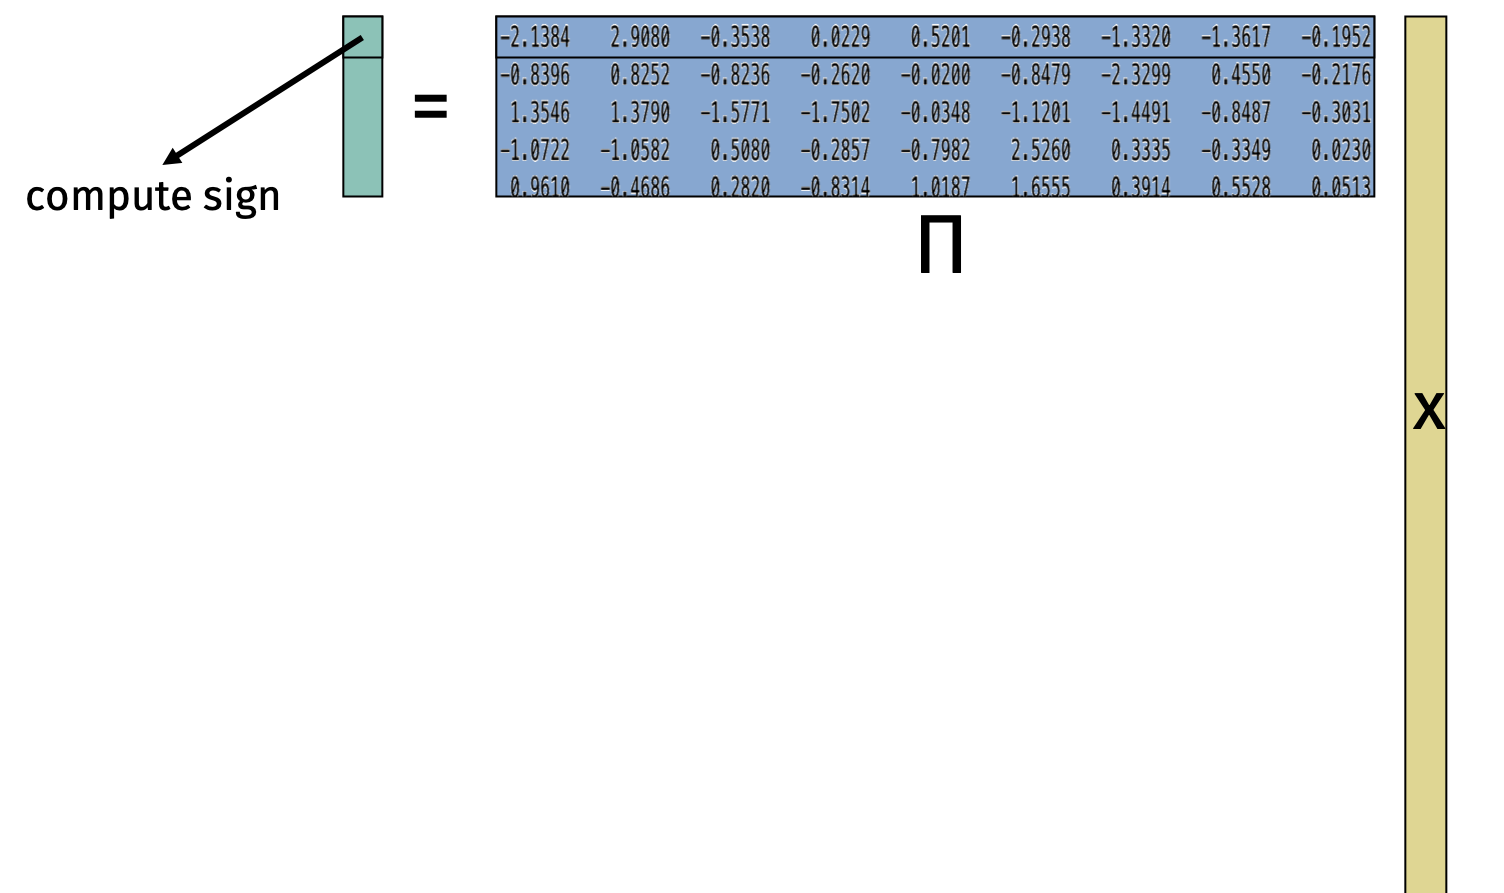
\includegraphics[width=\textwidth]{simhash_jl.png}
%	\end{center}
%\end{frame}



\begin{frame}[t]
	\frametitle{simhash analysis in 2d}
	\textbf{Theorem (to be prove):} If $\cos(\theta(\bv{x},\bv{y})) = v$, then 
	\begin{align*}
		\Pr[h(\bv{x}) == h(\bv{y})] = 1 - \frac{\theta}{\pi}  + \frac{1}{m}= 1 - \frac{\cos^{-1}(v)}{\pi} + \frac{1}{m}
	\end{align*}
	\begin{center}
		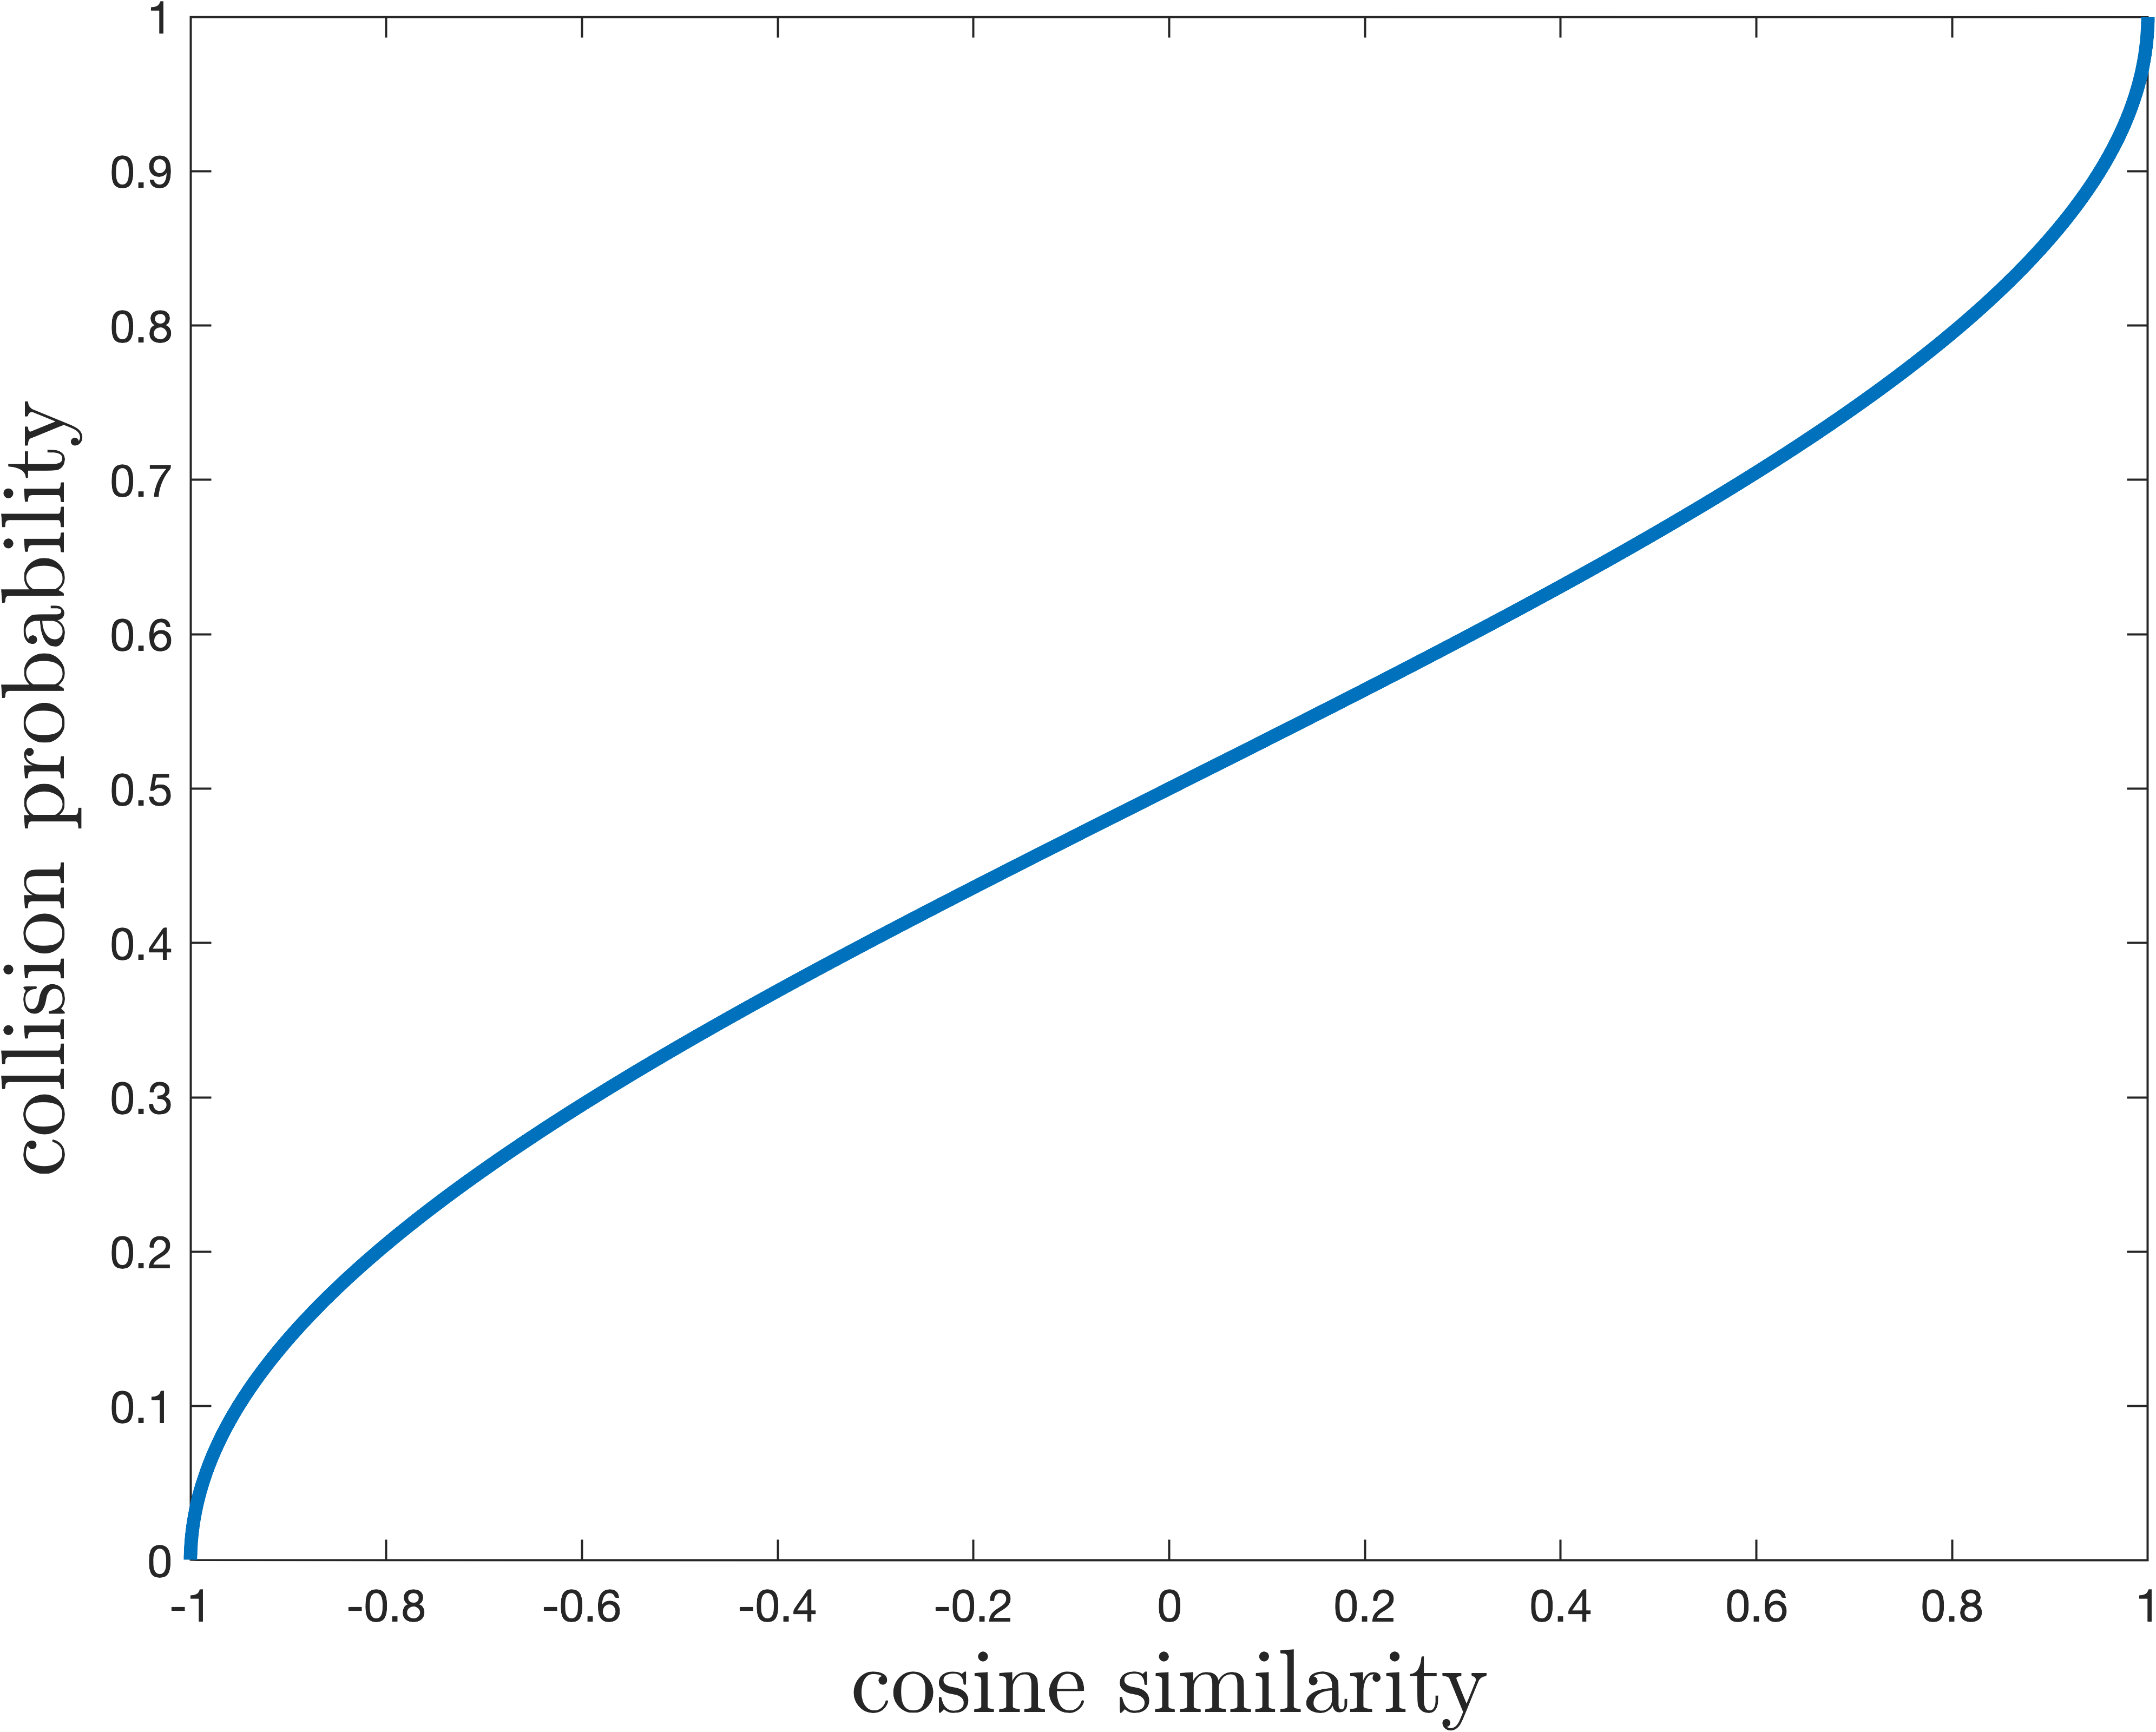
\includegraphics[width=.6\textwidth]{cosine_sim.png}
	\end{center}
\end{frame}

\begin{frame}
	\frametitle{simhash}
	SimHash can be tuned, just like our MinHash based LSH function for Jaccard similarity:
	\begin{itemize}
		\item Let $\bv{g}_1,\ldots, \bv{g}_r \in \R^d$ be randomly chosen with each entry $\mathcal{N}(0,1)$. 
		\item Let $f: \{-1,1\}^r \rightarrow \{1,\ldots, m\}$ be a uniformly random hash function. 
		\item $h: \R^d \rightarrow \{1,\ldots, m\}$ is defined $h(\bv{x}) = f\left([\sign(\langle \bv{g}_1, \bv{x} \rangle),\ldots, \sign(\langle \bv{g}_r, \bv{x} \rangle)]\right)$.
	\end{itemize}
\begin{align*}
	\Pr[h(\bv{x}) == h(\bv{y})] = \left(1-\frac{\theta}{\Pi}\right)^r
\end{align*}
\end{frame}

\begin{frame}
	\textbf{To prove:}  $\Pr[h(\bv{x}) == h(\bv{y})] = 1 - \frac{\theta}{\pi}$,  where $h(\bv{x}) = f\left(\sign(\langle \bv{g}, \bv{x} \rangle)\right)$ and $f$ is uniformly random hash function.
	\frametitle{simhash analysis in 2d}
	\vspace{-.5em}
	\begin{center}
		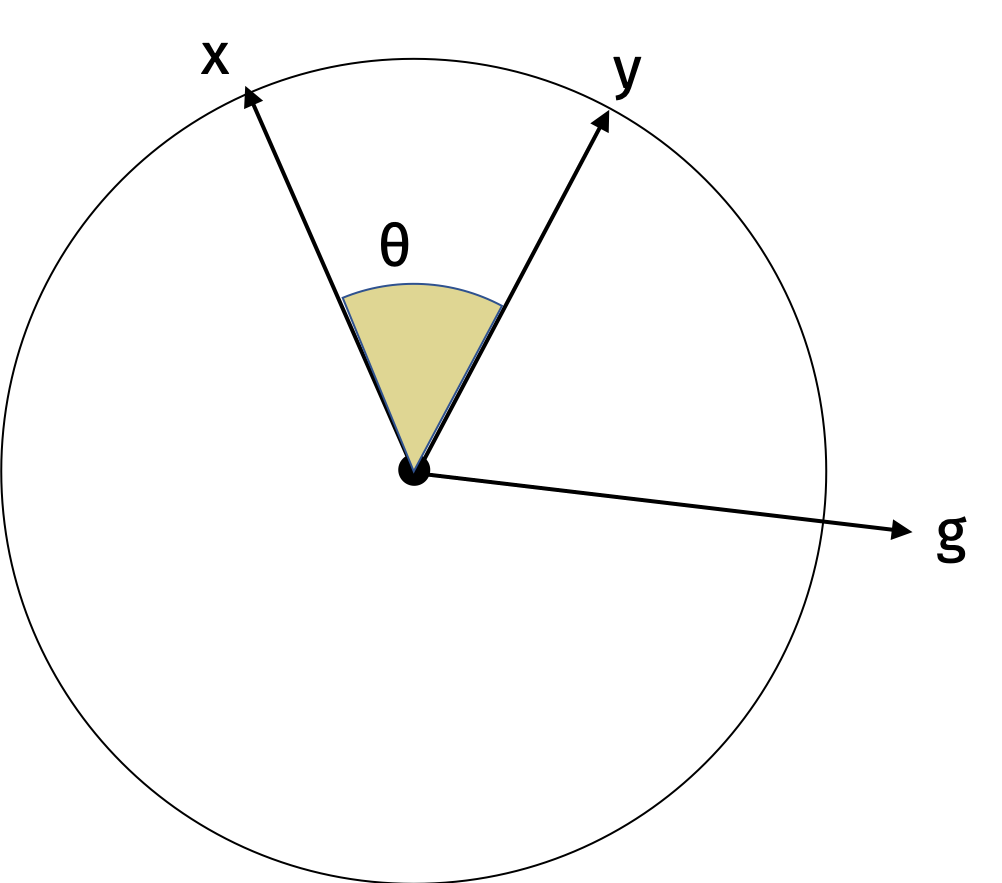
\includegraphics[width=.5\textwidth]{simhash1.png}
	\end{center}
\begin{align*}
	\Pr[h(\bv{x}) == h(\bv{y})] = z + \frac{1-v}{m} \approx z.
\end{align*}
where $z = \Pr[\sign(\langle \bv{g}, \bv{x} \rangle) == \sign(\langle \bv{g}, \bv{y} \rangle)]$
\end{frame}

\begin{frame}
	\frametitle{simhash analysis 2d}
	\vspace{-.5em}
	\begin{center}
		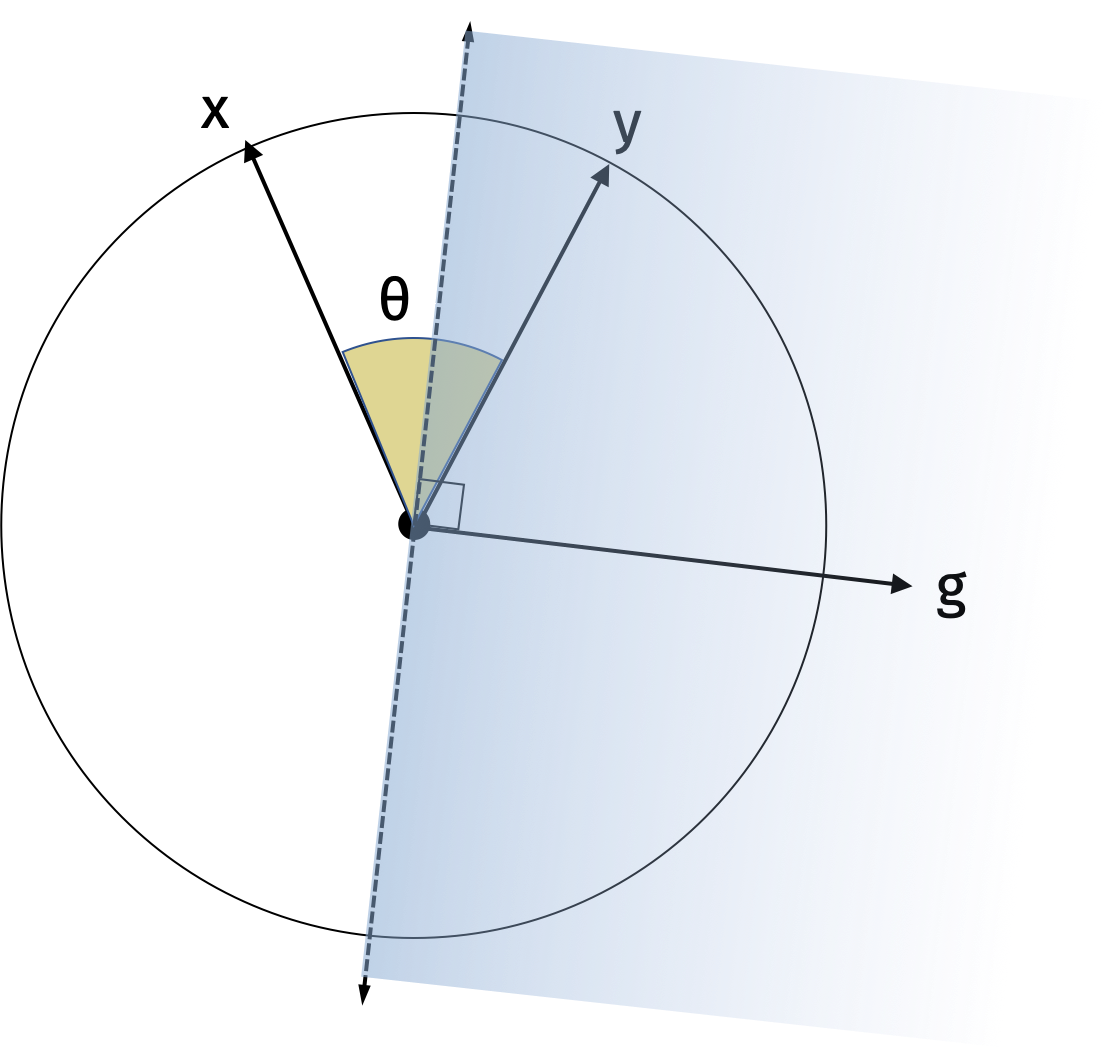
\includegraphics[width=.55\textwidth]{simhash2.png}
	\end{center}
\vspace{-.5em}
$\Pr[h(\bv{x}) == h(\bv{y})] \approx$ probability $\bv{x}$ and $\bv{y}$ are on the same side of hyperplane orthogonal to $\bv{g}$.
\end{frame}

\begin{frame}
	\frametitle{simhash analysis higher dimensions}
	\begin{center}
		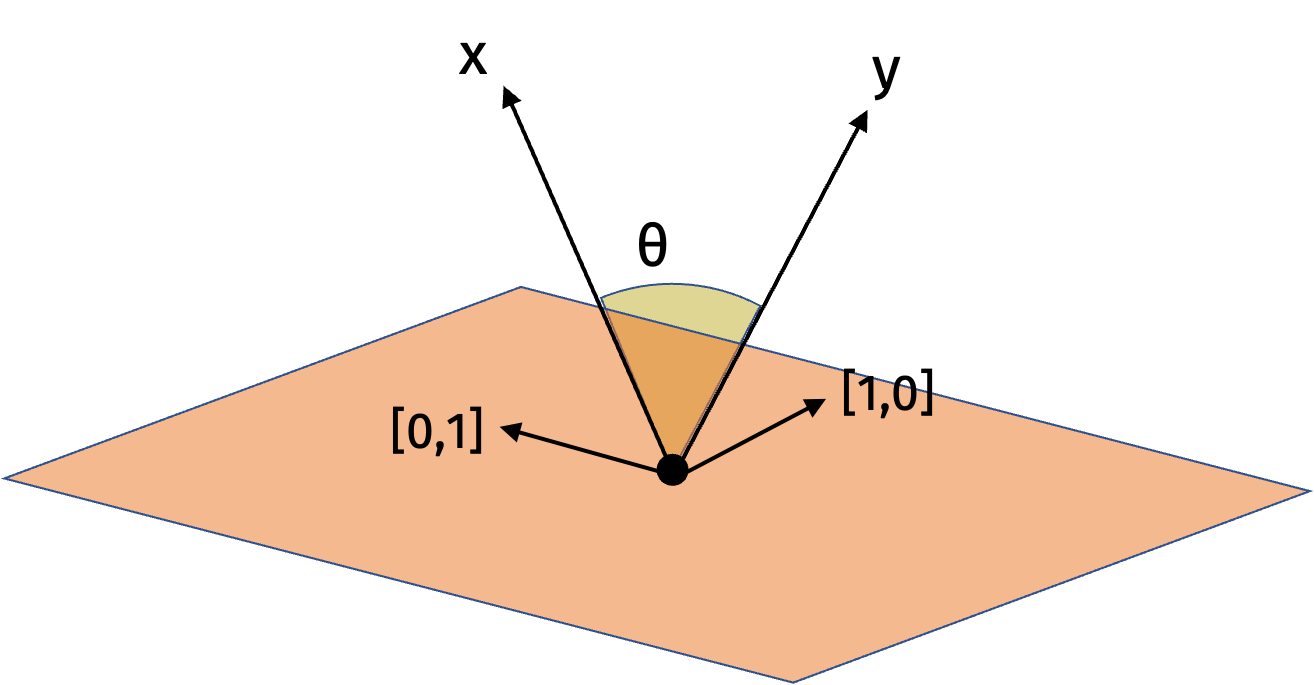
\includegraphics[width=.7\textwidth]{high_dim1.png}
	\end{center}
There is always some \emph{rotation matrix} $\bv{U}$ such that $\bv{U}\bv{x},\bv{U}\bv{y}$ are spanned by the first two-standard basis vectors and have the same cosine similarity as $\bv{x}$ and $\bv{y}$.
\end{frame}

\begin{frame}
	\frametitle{simhash analysis higher dimensions}
	\begin{center}
		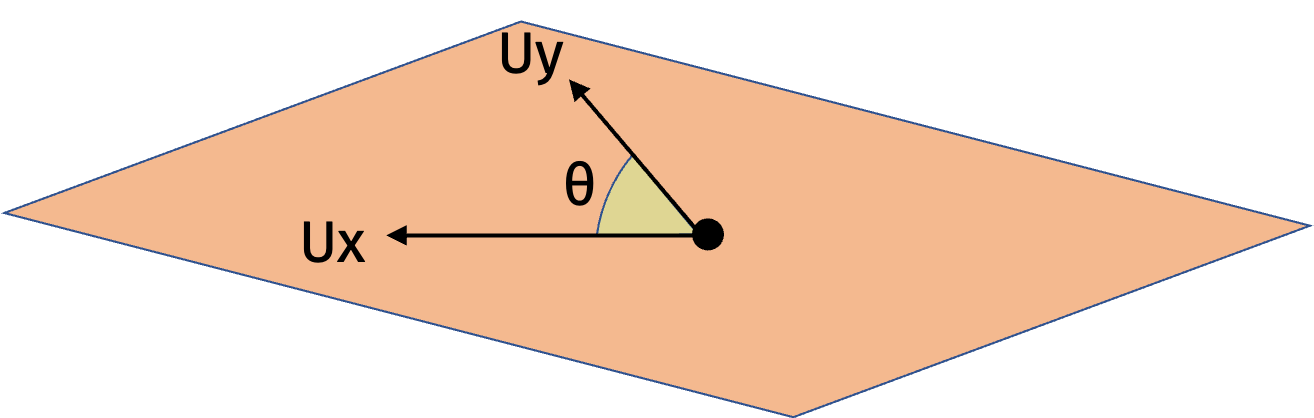
\includegraphics[width=.7\textwidth]{high_dim2.png}
	\end{center}
	There is always some \emph{rotation matrix} $\bv{U}$ such that $\bv{x},\bv{y}$ are spanned by the first two-standard basis vectors. 
	
	
	\textbf{Note:} A rotation matrix $\bv{U}$ has the property that $\bv{U}^T\bv{U} = \bv{I}$. I.e., $\bv{U}^T$ is a rotation matrix itself, which reverses the rotation of $\bv{U}$.
\end{frame}

\begin{frame}[t]
	\frametitle{simhash analysis higher dimensions}
\textbf{Claim:} 
\begin{align*}
1 - \frac{\theta}{\pi} &= \Pr[\sign(\langle \bv{g}[1,2], (\bv{U}\bv{x})[1,2] \rangle) == \sign(\langle \bv{g}[1,2], (\bv{U}\bv{y}[1,2] \rangle)] \\
&= \Pr[\sign(\langle \bv{g}, \bv{U}\bv{x} \rangle) == \sign(\langle \bv{g}, \bv{U}\bv{y} \rangle)] \\
&\alert{= \Pr[\sign(\langle \bv{g}, \bv{x} \rangle) == \sign(\langle \bv{g}, \bv{y} \rangle)]}
\end{align*}

	Why?
\end{frame}

\begin{frame}[t]
	\frametitle{modern near neigbhor search}
	\begin{itemize}
		\item High-dimensional vector search is exploding as a research area with the rise of machine-learned multi-modal embeddings for images, text, and more. 
	\end{itemize}
	\begin{center}
		\vspace{-.5em}
				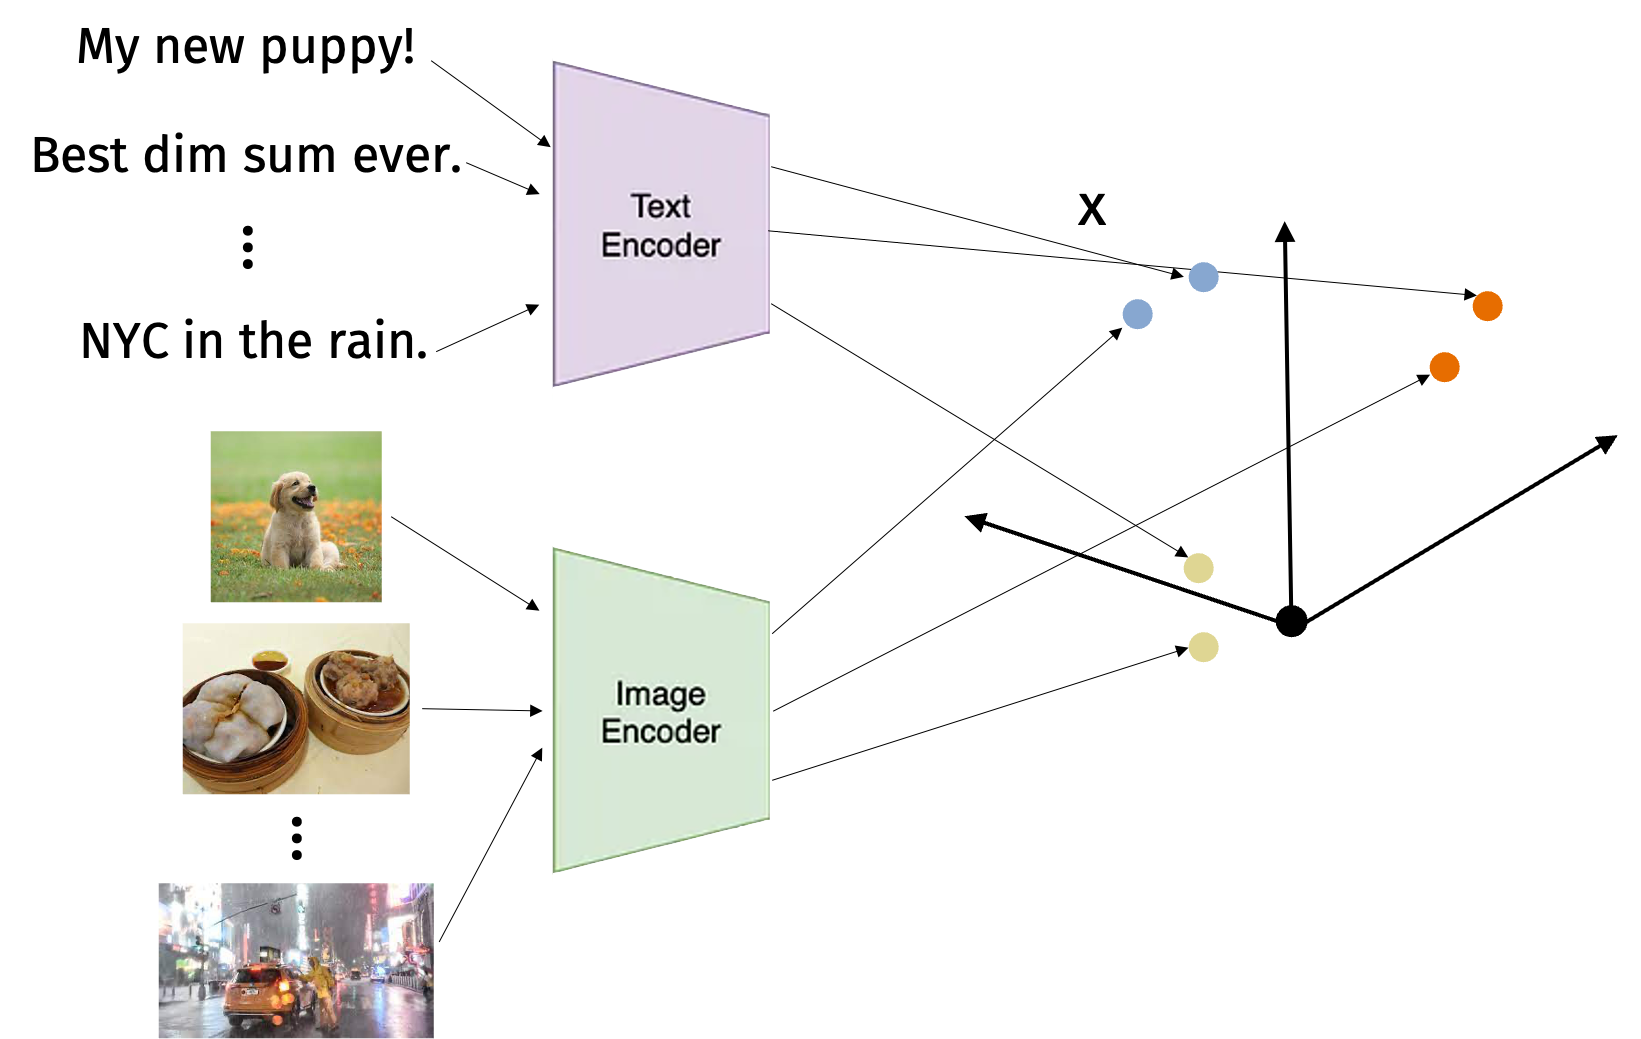
\includegraphics[width=.8\textwidth]{multimodal_embeddings.png}
				\vspace{-.5em}
	\end{center}
	Web-scale image search is now a vector search problem. 
\end{frame}

\begin{frame}[t]
	\frametitle{graph based near neigbhor}
	
\end{frame}

%\begin{frame}[standout]
%	\begin{center}
%		break
%	\end{center}
%\end{frame}
%
%\begin{frame}
%	\frametitle{next unit: continuous optimization}
%	Have some function $f : \R^d \rightarrow \R$. Want to find ${\bv{x}}^*$ such that:
%	\begin{align*}
%		f({\bv{x}}^*) = \min_{\bv{x}} f(\bv{x}).
%	\end{align*}
%	Or at least $\hat{\bv{x}}$ which is close to a minimum. E.g. $f(\hat{\bv{x}}) \leq \min_{\bv{x}} f(\bv{x}) + \epsilon$
%	
%	Often we have some additional constraints:
%	\begin{itemize}
%		\item $\bv{x} > 0$.
%		\item $\|\bv{x}\|_2 \leq R$, $\|\bv{x}\|_1 \leq R$.
%		\item $\bv{a}^T\bv{x} > c$.
%	\end{itemize}
%\end{frame}
%
%\begin{frame}
%	\frametitle{continuous optimization}
%	\textbf{Dimension $d = 1$:}
%	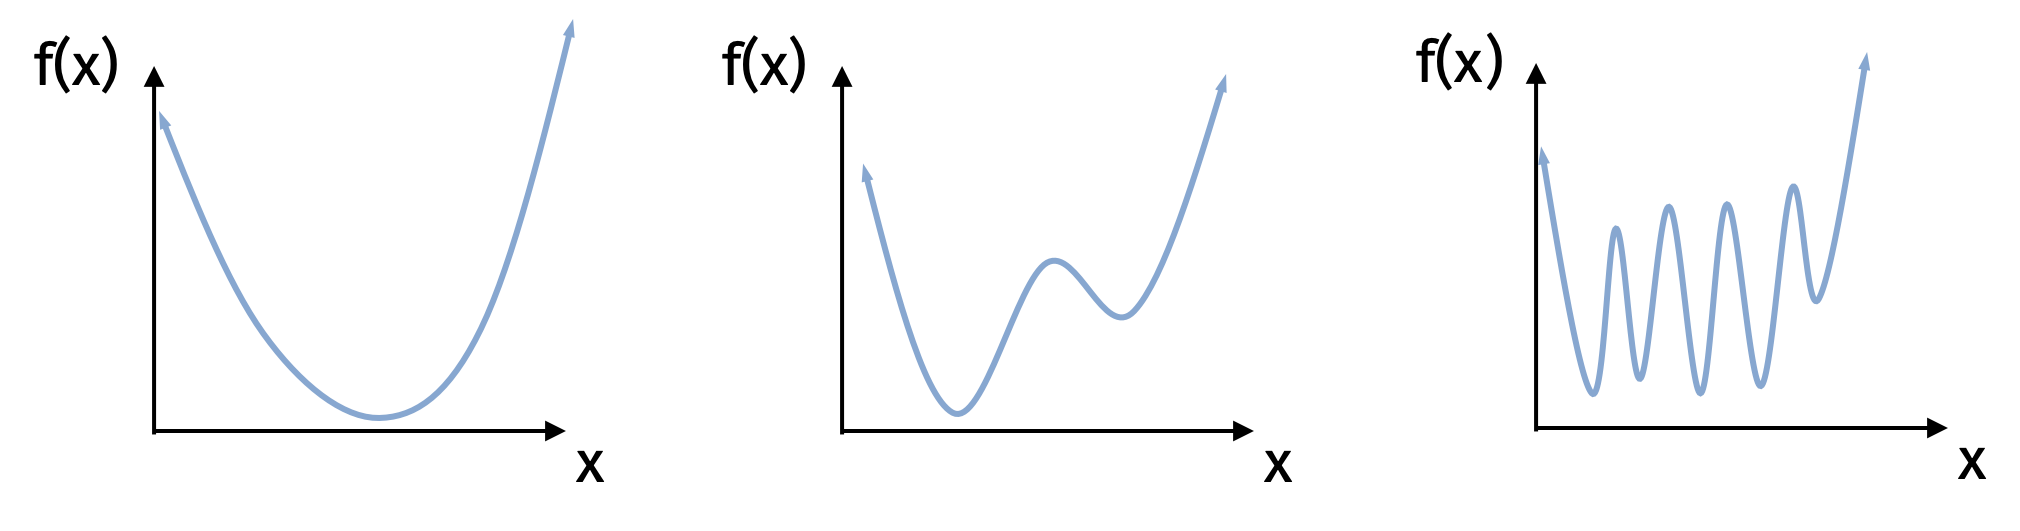
\includegraphics[width=\textwidth]{1d_functions.png}
%	
%	\textbf{Dimension $d = 2$:}
%	
%	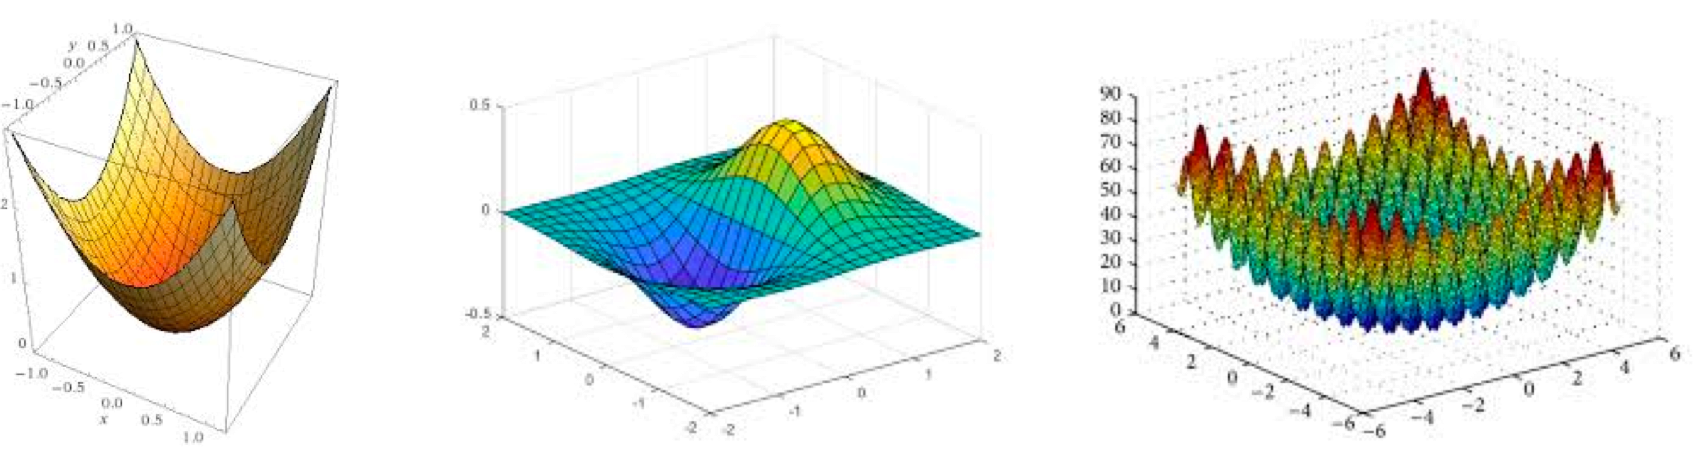
\includegraphics[width=\textwidth]{2dfunctions.png}
%\end{frame}
%
%\begin{frame}
%	\frametitle{optimization in machine learning}
%	\begin{center}
%		\alert{\textbf{Continuouos optimization is the foundation of modern machine learning.}}
%	\end{center}
%	\textbf{Supervised learning:} Want to learn a model that maps \emph{inputs}
%	\begin{itemize}
%		\item numerical data vectors
%		\item images, video
%		\item text documents
%	\end{itemize} 
%	
%	to \emph{predictions}
%	\begin{itemize}
%		\item numerical value (probability stock price increases)
%		\item label (is the image a cat? does the image contain a car?)
%		\item decision (turn car left, rotate robotic arm)
%	\end{itemize} 
%\end{frame}
%
%\begin{frame}
%	\frametitle{machine learning model}
%	\begin{center}
%		Let $M_{\bv{x}}$ be a model with parameters $\bv{x} = \{x_1, \ldots, x_k\}$, which takes as input a data vector $\bv{a}$ and outputs a prediction.
%	\end{center}
%	
%	\textbf{Example:}
%	\begin{align*}
%		M_{\bv{x}}(\bv{a}) = \sign(\bv{a}^T\bv{x})
%	\end{align*}		
%\end{frame}
%
%\begin{frame}[t]
%	\frametitle{machine learning model}
%	\textbf{Example:}
%	\begin{center}
%		\includegraphics[width=.7\textwidth]{neuralNetwork.png}
%	\end{center}	
%	$\bv{x}\in \R^{\text{(\# of connections)}}$ is the parameter vector containing all the network weights. 	
%\end{frame}
%
%\begin{frame}
%	\frametitle{supervised learning}
%	Classic approach in \emph{supervised learning}: Find a model that works well on data that you already have the answer for (labels, values, classes, etc.).
%	\begin{itemize}
%		\item Model $M_{\bv{x}}$ parameterized by a vector of numbers $\bv{x}$.
%		\item Dataset $\bv{a}^{(1)}, \ldots,  \bv{a}^{(n)}$ with outputs $y^{(1)}, \ldots, y^{(n)}$.
%	\end{itemize}
%	\begin{center}
%		Want to find $\hat{\bv{x}}$ so that $M_{\hat{\bv{x}}}(\bv{a}^{(i)}) \approx y^{(i)}$ for $i \in 1,\ldots, n$.
%		
%		\alert{\textbf{How do we turn this into a function minimization problem?}}
%	\end{center}
%\end{frame}
%
%\begin{frame}
%	\frametitle{loss function}
%	\textbf{Loss function $L\left(M_{\bv{x}}(\bv{a}), y\right)$:} Some measure of distance between prediction $M_{\bv{x}}(\bv{a})$ and target output $y$. Increases if they are further apart.
%	\begin{itemize}
%		\item Squared ($\ell_2$) loss: $|M_{{\bv{x}}}(\bv{a}) - y|^2$
%		\item Absolute deviation ($\ell_1$) loss: $|M_{{\bv{x}}}(\bv{a}) - y|$
%		\item Hinge loss: 1 - $y \cdot M_{{\bv{x}}}(\bv{a})$ 
%		\item Cross-entropy loss (log loss). 
%		%		$−o  \log(M_{{\bv{x}}}(\bv{y})+(1 - o)\log(1 - M_{{\bv{x}}}(\bv{y}))$
%		\item Etc.
%	\end{itemize}
%\end{frame}
%
%\begin{frame}
%	\frametitle{empirical risk minimization}
%	\textbf{Empirical risk minimization}:
%	\begin{align*}
%		f(\bv{x}) = \sum_{i=1}^n L\left(M_{\bv{x}}(\bv{a}^{(i)}), y^{(i)}\right)
%	\end{align*}
%	\begin{center}
%		Solve the optimization problem $\min_{\bv{x}} f(\bv{x})$.
%	\end{center}
%\end{frame}
%
%\begin{frame}
%	\frametitle{example: linear regression}
%	\begin{itemize}
%		\item $M_{\bv{x}}(\bv{a}) = \bv{x}^T\bv{a}$. $\bv{x}$ contains the regression coefficients. 
%		\item $L(z,y) = |z-y|^2$. 
%		\item $f(\bv{x}) = \sum_{i=1}^n |\bv{x}^T\bv{a}^{(i)} - y^{(i)}|^2$
%	\end{itemize}
%	\begin{align*}
%		f(\bv{x}) = \|\bv{A}\bv{x} - \bv{y}\|_2^2
%	\end{align*}
%	where $\bv{A}$ is a matrix with $\bv{a}^{(i)}$ as its $i^\text{th}$ row and $\bv{y}$ is a vector with $y^{(i)}$ as its $i^\text{th}$ entry. 
%\end{frame}
%
%\begin{frame}
%	\frametitle{algorithms for continuous optimization}
%	The choice of algorithm to minimize $f(\bv{x})$ will depend on:
%	\begin{itemize}
%		\item The form of $f(\bv{x})$ (is it linear, is it quadratic, does it have finite sum structure, etc.)
%		\item If there are any additional constraints imposed on $\bv{x}$. E.g. $\|\bv{x}\|_2 \leq c$. 
%	\end{itemize}
%	\textbf{What are some example algorithms for continuous optimization?}
%	
%\end{frame}
%
%\begin{frame}
%	\frametitle{first topic: gradient descent + variants}
%	\textbf{Gradient descent:} A greedy algorithm for minimizing functions of multiple variables that often works amazingly well. 
%	\begin{center}
%		\includegraphics[width=.4\textwidth]{greedy_gradient.png}
%		
%		Runtime generally scales \emph{linearly} with the dimension of $\bv{x}$ (although this is a bit of an over-simplification).
%	\end{center}
%\end{frame}
%
%\begin{frame}
%	\frametitle{second topic: methods suitable for lower dimension }
%	\begin{itemize}
%		\item Cutting plane methods (e.g. center-of-gravity, ellipsoid)
%		\item Interior point methods
%	\end{itemize}
%	Fast and more accurate in low-dimensions, slower in very high dimensions. Generally runtime scales \emph{polynomially} with the dimension of $\bv{x}$.
%\end{frame}
%
%\begin{frame}
%	\frametitle{calculus review}
%	For $i = 1, \ldots, d$, let $x_i$ be the $i^\text{th}$ entry of $\bv{x}$. Let $\bv{e}^{(i)}$ be the $i^\text{th}$ \emph{standard basis vector.}
%	\vspace{2em}
%	
%	\textbf{Partial derivative:}
%	\begin{align*}
%		\frac{\partial f}{\partial x_i}(\bv{x}) = \lim_{t\rightarrow 0} \frac{f(\bv{x} + t\bv{e}^{(i)}) - f(\bv{x})}{t}
%	\end{align*}
%	\textbf{Directional derivative:}
%	\begin{align*}
%		D_\bv{v}f(\bv{x}) = \lim_{t\rightarrow 0} \frac{f(\bv{x} + t\bv{v}) - f(\bv{x})}{t}
%	\end{align*}
%\end{frame}
%
%\begin{frame}
%	\frametitle{calculus review}
%	\textbf{Gradient}:
%	\begin{align*}
%		\nabla f(\bv{x}) = 
%		\begin{bmatrix}
%			\frac{\partial f}{\partial x_1}(\bv{x}) \\ \frac{\partial f}{\partial x_2}(\bv{x}) \\ \vdots \\ \frac{\partial f}{\partial x_d}(\bv{x}) 
%		\end{bmatrix}
%	\end{align*}
%	\textbf{Directional derivative:}
%	\begin{align*}
%		D_\bv{v}f(\bv{x}) = \lim_{t\rightarrow 0} \frac{f(\bv{x} + t\bv{v}) - f(\bv{x})}{t} = \alert{\nabla f(\bv{x})^T \bv{v}.}
%	\end{align*}
%\end{frame}
%
%
%\begin{frame}
%	\frametitle{first order optimization}
%	Given a function $f$ to minimize, assume we have:
%	\begin{itemize}
%		\item \textbf{Function oracle}: Evaluate $f(\bv{x})$ for any $\bv{x}$. 
%		\item \textbf{Gradient oracle}: Evaluate $\nabla f(\bv{x})$ for any $\bv{x}$.
%	\end{itemize}
%	We view the implementation of these oracles as black-boxes, but they can often require a fair bit of computation. 
%\end{frame}
%
%\begin{frame}[t]
%	\frametitle{example gradient evaluation}
%	\textbf{Linear least-squares regression}:
%	\begin{itemize}
%		\item Given $\bv{a}^{(1)}, \ldots \bv{a}^{(n)} \in \R^d$, ${y}^{(1)}, \ldots {y}^{(n)} \in \R$.
%		\item Want to minimize:
%		\begin{align*}
%			f(\bv{x}) = \sum_{i=1}^n \left(\bv{x}^T\bv{a}^{(i)} - {y}^{(i)}\right)^2 = \|\bv{A}\bv{x} - \bv{y}\|_2^2.
%		\end{align*} 
%	\end{itemize}
%	
%	\begin{align*}
%		\frac{\partial f}{\partial x_j} = \sum_{i=1}^n 2\left(\bv{x}^T\bv{a}^{(i)} - {y}^{(i)}\right)\cdot a^{(i)}_j = (2\bv{A}\bv{x} -\bv{y})^T\bs{\alpha}^{(j)}
%	\end{align*}
%	where $\bs{\alpha}^{(j)}$ is the $j^\text{th}$ \emph{column} of $\bv{A}$. 
%	\begin{align*}
%		\nabla f(\bv{x}) = 2\bv{A}^T\left(\bv{A}\bv{x} - \bv{y}\right)
%	\end{align*}
%	\textbf{What is the time complexity of a gradient oracle for $\nabla f(\bv{x})$?}
%\end{frame}
%
%\begin{frame}
%	\frametitle{decent methods}
%	\textbf{Greedy approach:} Given a starting point $\bv{x}$, make a small adjustment that decreases $f(\bv{x})$. In particular, $\bv{x} \leftarrow \bv{x} + \eta\bv{v}$ and $f(\bv{x}) \leftarrow f(\bv{x} + \eta\bv{v})$.
%	
%	\begin{center}
%		\alert{What property do I want in $\bv{v}$?}
%	\end{center}
%	
%	
%	\textbf{Leading question:} When $\eta$ is small, what's an approximation for $f(\bv{x} + \eta\bv{v}) - f(\bv{x})$?
%	\begin{align*}
%		f(\bv{x} + \eta\bv{v}) - f(\bv{x}) \approx \hspace{6em}
%	\end{align*}
%	
%	
%\end{frame}
%
%\begin{frame}[t]
%	\frametitle{directional derivatives}
%	
%	\begin{align*}
%		D_\bv{v}f(\bv{x}) = \lim_{t\rightarrow 0} \frac{f(\bv{x} + t\bv{v}) - f(\bv{x})}{t} = \nabla f(\bv{x})^T \bv{v}.
%	\end{align*}	
%	So:
%	\begin{align*}
%		f(\bv{x} + \eta\bv{v}) - f(\bv{x}) \approx \hspace{6em}
%	\end{align*}
%	
%	\textbf{How should we choose $\bv{v}$ so that $f(\bv{x} + \eta\bv{v}) < f(\bv{x})$?} 
%	
%\end{frame}
%
%\begin{frame}
%	\frametitle{gradient descent}
%	\textbf{Prototype algorithm:}
%	\begin{itemize}
%		\item Choose starting point $\bv{x}^{(0)}$.
%		\item For $i = 0,\ldots, T$:
%		\begin{itemize}
%			\item $\bv{x}^{(i+1)} = \bv{x}^{(i)} - \eta \nabla f(\bv{x}^{(i)})$
%		\end{itemize}
%		\item Return $\bv{x}^{(T)}$.
%	\end{itemize}
%	
%	$\eta$ is a step-size parameter, which is often adapted on the go. For now, assume it is fixed ahead of time.
%\end{frame}
%
%\begin{frame}[t]
%	\frametitle{gradient descent intuition}
%	\textbf{1 dimensional example:}
%\end{frame}
%
%\begin{frame}[t]
%	\frametitle{gradient descent intuition}
%	\textbf{2 dimensional example:}
%	\begin{center}
%		\includegraphics[width=.7\textwidth]{2d_example.png}
%	\end{center}
%\end{frame}
%
%\begin{frame}[t]
%	\frametitle{key results}
%	\textbf{For a convex function $f(\bv{x})$:}
%	For sufficiently small $\eta$ and a sufficiently large number of iterations $T$, gradient descent will converge to a \alert{\textbf{near global minimum}}:
%	\begin{align*}
%		f(\bv{x}^{(T)}) \leq  f(\bv{x}^{*}) + \epsilon.  
%	\end{align*}
%	Examples: least squares regression, logistic regression, kernel regression, SVMs.
%	
%	\textbf{For a non-convex function $f(\bv{x})$:}
%	For sufficiently small $\eta$ and  a sufficiently large number of iterations $T$, gradient descent will converge to a \alert{\textbf{near stationary point}}:
%	\begin{align*}
%		\|\nabla f(\bv{x}^{(T)})\|_2 \leq  \epsilon.  
%	\end{align*}
%	Examples: neural networks, matrix completion problems, mixture models. 	
%\end{frame}
%
%\begin{frame}[t]
%	\frametitle{convex vs. non-convex}
%	\begin{center}
%		\includegraphics[width=\textwidth]{nonconvex_converge.png}
%	\end{center}
%	One issue with non-convex functions is that they can have \alert{\textbf{local minima}}. Even when they don't, convergence analysis requires different assumptions than convex functions. 	
%\end{frame}
%
%\begin{frame}[t]
%	\frametitle{approach for this unit}
%	We care about \emph{how fast} gradient descent and related methods converge, not just that they do converge. 
%	\begin{itemize}
%		\item Bounding iteration complexity requires placing some assumptions on $f(\bv{x})$. 
%		\item Stronger assumptions lead to better bounds on the convergence. 
%	\end{itemize}
%	Understanding these assumptions can help us design faster variants of gradient descent (there are many!). 
%\end{frame}
%
%\begin{frame}[t]
%	\frametitle{convexity}
%	\begin{definition}[Convex]
%		A function $f$ is convex iff for any $\bv{x}, \bv{y},\lambda \in [0,1]$:
%		\begin{align*}
%			(1-\lambda)\cdot f(\bv{x}) + \lambda \cdot f(\bv{y}) \geq f\left((1-\lambda)\cdot\bv{x} + \lambda \cdot\bv{y}\right)
%		\end{align*}
%	\end{definition}
%	\vspace{-.5em}
%	\begin{center}
%		\includegraphics[width=.6\textwidth]{convex1.png}
%	\end{center}
%\end{frame}
%
%
%\begin{frame}[t]
%	\frametitle{gradient descent}
%	\small
%	\begin{definition}[Convex]
%		A function $f$ is convex if and only if for any $\bv{x}, \bv{y}$:
%		\begin{align*}
%			f(\bv{x} + \bv{z}) \geq f(\bv{x}) + \nabla f(\bv{x})^T\bv{z}
%		\end{align*}
%		\vspace{-1em}
%		Equivalently:
%		\vspace{-.5em}
%		\begin{align*}
%			f(\bv{x}) - f(\bv{y}) \leq \nabla f(\bv{x})^T (\bv{x} - \bv{y})
%		\end{align*}
%		\vspace{-1em}
%	\end{definition}
%	
%	\includegraphics[width=.5\textwidth]{convex2.png}
%	
%\end{frame}
%
%\begin{frame}[t]
%	\frametitle{gradient descent analysis}
%	\textbf{Assume:}
%	\begin{itemize}
%		\item $f$ is convex.
%		\item Lipschitz function: for all $\bv{x}$, $\|\nabla f(\bv{x})\|_2 \leq \alert{G}$.
%		\item Starting radius: $\|\bv{x}^{*} - \bv{x}^{(0)}\|_2 \leq \alert{R}$.
%	\end{itemize}
%	
%	\textbf{Gradient descent:}
%	\begin{itemize}
%		\item Choose number of steps $T$.
%		\item Starting point $\bv{x}^{(0)}$. E.g.  $\bv{x}^{(0)} = \vec{0}$.
%		\item $\eta = \frac{R}{G\sqrt{T}}$
%		\item For $i = 0,\ldots, T$:
%		\begin{itemize}
%			\item $\bv{x}^{(i+1)} = \bv{x}^{(i)} - \eta \nabla f(\bv{x}^{(i)})$
%		\end{itemize}
%		\item Return $\hat{\bv{x}} = \argmin_{\bv{x}^{(i)}} f(\bv{x}^{(i)})$.
%		%		\item Alternatively, return $\hat{\bv{x}} = \frac{1}{T}\sum_{i=1}^T \bv{x}^{(i)}$.
%	\end{itemize}
%\end{frame}

\end{document} 








